\documentclass{article}  % Tipo di documento
\usepackage[utf8]{inputenc} % Per caratteri accentati
\usepackage[italian]{babel} % Lingua italiana
\usepackage{amsthm}
\usepackage{amssymb}
\usepackage{amsmath}  % simboli matematici avanzati
\usepackage{xcolor} % Per i colori
\usepackage{titlesec} % Per personalizzare i titoli
\usepackage{tikz}
\usetikzlibrary{mindmap,trees}
\usepackage[most]{tcolorbox}
\usepackage{subcaption}  % per avere subfigure
\tcbuselibrary{theorems}
\usepackage{tikz}
\usetikzlibrary{automata, positioning, arrows}
\tcbuselibrary{breakable}
\usepackage{graphicx}
\usepackage[table]{xcolor} % da mettere nel preambolo
\usepackage{mathrsfs} % https://www.ctan.org/pkg/mathrsfs
\graphicspath{ {./media/} }

\usepackage[hidelinks]{hyperref}  % <<--- SPOSTALA QUI


\newtcbtheorem[no counter]{theorem}{Teorema}%
{colback=blue!5, 
colframe=blue!50!black, 
fonttitle=\bfseries,
    breakable,            % permette di spezzare il box su più pagine
    enhanced,
    break at=0pt}{}

\theoremstyle{definition}
\newtheorem{definition}{Definizione}[section]

% Imposto colore delle subsection
\titleformat{\subsection}
  {\normalfont\large\color{red}} % stile del titolo
  {\thesubsection}{1em}{} % numerazione e spaziatura

% Definiamo un nuovo ambiente per gli esempi
\newtcolorbox{esempio}[1][]{
    colback=white,       % colore di sfondo
    colframe=gray,       % colore del bordo
    fonttitle=\bfseries,
    title=#1,
    boxrule=0.5pt,       % spessore del bordo
    arc=4pt,             % angoli arrotondati
    left=4pt, right=4pt, top=4pt, bottom=4pt,
	breakable,            % permette di spezzare il box su più pagine
    enhanced,
    break at=0pt
}

\newtcolorbox{esercizio}[1][]{
    colback=white,       % colore di sfondo
    colframe=green!60!black,       % colore del bordo
    fonttitle=\bfseries,
    title=#1,
    boxrule=0.5pt,       % spessore del bordo
    arc=4pt,             % angoli arrotondati
    left=4pt, right=4pt, top=4pt, bottom=4pt,
    breakable,            % permette di spezzare il box su più pagine
    enhanced,
    break at=0pt
}

\newtcolorbox{osservazioni}[1][]{
    colback=white,       % colore di sfondo
    colframe=yellow!80!orange,       % colore del bordo
    fonttitle=\bfseries,
    title=#1,
    boxrule=0.5pt,       % spessore del bordo
    arc=4pt,             % angoli arrotondati
    left=4pt, right=4pt, top=4pt, bottom=4pt,
    breakable,            % permette di spezzare il box su più pagine
    enhanced,
    break at=0pt
}

% Creo un nuovo ambiente "ragionamento" senza quadratino
\newenvironment{ragionamento}[1][]
  {\begin{proof}[Ragionamento#1]\renewcommand{\qedsymbol}{}\normalfont}
  {\end{proof}}

\title{Informatica Teorica}
\author{Ede Boanini}
\date{\today}

\begin{document}
\maketitle
\tableofcontents % genera automaticamente l’indice
\newpage
%%%%%%%%%%%%%%%%%%%%%%%%%%%%%%%%%%%%%%%%%%%%%%%%%%%%%%%%%%%%%%%%%%%%%%%%%%%%%%%%%%%%%%%%%%%%%%%%%%%%%%
\section{Introduzione}
\subsection{Definizioni essenziali}
\begin{definition}[Grafo]
	Sia \(G=(V,E)\) un grafo non orientato, dove:
	\begin{itemize}
		\item \(V\) è l'insieme dei nodi
		\item \(E\) è l'insieme degli archi
	\end{itemize}
\end{definition}
\begin{definition}[Coppia di nodi]
	Siano \(u\) e \(v\) due nodi di un grafo \(G = (V,E)\).
	La coppia \(\{u,v\}\) rappresenta un arco che connette i nodi \(u\) e \(v\).
\end{definition}
\begin{definition}[Grado di un nodo]
	Numero di archi che collegano un nodo $v$ ad altri nodi.
	\[
		deg(v)=k
	\]
\end{definition}
\begin{definition}[Grafo $k$-regolare]
	Un grafo \(G=(V,E)\) è $k$-regolare se ogni nodo ha grado $k$:
	\[
		\forall v \in V, \quad deg(v)=k
	\]
\end{definition}
%%%%%%%%%%%%%%%%%%%%%%%%%%%%%%%%%%%%%%%%%%%%%%%%%%%%%%%%%%%%%%%%%%%%%%%%%%%%%%%%%%%%%%%%%%%%%%%%%%%%%%
\subsection{Leggi di De Morgan}
%%%%%%%%%%%%%%%%%%%%%%%%%%%%%%%%%%%%%%%%%%%%%%%%%%%%%%%%%%%%%%%%%%%%%%%%%%%%%%%%%%%%%%%%%%%%%%%%%%%%%%
\subsection{Tipi di dimostrazioni}
\begin{tikzpicture}[
		level 1/.style={
				sibling distance=40mm,
				level distance=20mm,
				every node/.append style={font=\small} % qui riduco il font dei figli
			},
		every node/.style={
				rectangle, draw, rounded corners,
				align=center,
				top color=blue!20,
				bottom color=blue!10
			}
	]
	\node {Tipi di \\ dimostrazione}
	child {node {Per \\ costruzione}}
	child {node {Per \\ assurdo}}
	child {node {Per \\ induzione}};
\end{tikzpicture}

\begin{definition}[Dimostrazione per Costruzione]
	Il teorema afferma che esiste un particolare tipo di oggetto. Un modo per dimostrare un teorema di questo tipo è mostrare come costruire l’oggetto.
\end{definition}
\(\bigstar\) Idea: vuoi dimostrare che un oggetto esiste? Lo costruisci direttamente.


\begin{esempio}[Esempio]
	\footnotesize % riduce la dimensione del font
	Per ogni numero pari $n>2$, \(\exists\) un grafo $3$-regolare con $n$ nodi.
	\begin{proof}
		Sia $n$ un numero pari maggiore di 2. Costruisco un grafo \(G=(V,E)\) con $n$ nodi come segue:\newline
		Dispongo i nodi in cerchio. Collego ogni nodo con il successivo \(\{i,i+1\}\) formando un ciclo. Dopodichè collego ogni nodo con il suo opposto \(\{i,i+n/2\}\).
		In questo modo, ogni nodo ha 3 archi, quindi $G$ è $3$-regolare.
	\end{proof}
	Ho dimostrato il teorema costruendo un grafo che rispetta l'ipotesi (che il numero di nodi sia un numero pari maggiore di 2) arrivando poi alla tesi: ipotesi \(\rightarrow\) costruzione \(\rightarrow\) tesi.
\end{esempio}

\begin{definition}[Dimostrazione per Assurdo]
	Assumo che il teorema sia falso e mostro che questa assunzione conduce a una proposizione che è logicamente impossibile, cioè che contraddice un fatto già dimostrato o una proprietà nota. Questa contraddizione implica che l’assunzione iniziale era falsa, quindi il teorema è vero.
\end{definition}
\(\bigstar\) Idea: supponi che il teorema sia falso (neghi la tesi). Se questa assunzione porta ad un'assurdità, allora il teorema deve essere vero.

\begin{definition}[Dimostrazione per Induzione]
	Metodo usato per mostrare che tutti gli elementi di un insieme infinito possiedono una proprietà specifica. Questa dimostrazione
	consiste in due fasi:
	\begin{itemize}
		\item \textbf{Base:} dimostro che la proprietà \(\mathcal{P}\) vale per il primo elemento dell'insieme. Verifico che $\mathcal{P}(1)$ (oppure $\mathcal{P}(0)$, dipende da dove parte l'insieme) è vera.
		\item \textbf{Passo induttivo:} suppongo che, per ogni $k \geq 1$, la proprietà $\mathcal{P}(k)$ sia vera (ipotesi induttiva). Ciò implica che anche $\mathcal{P}(k+1)$ è vera.
	\end{itemize}

\end{definition}
\(\bigstar\) Idea: dimostri che una proprietà vale per infiniti casi.
\begin{esempio}[Esempio]
	\footnotesize % riduce la dimensione del font
	Per ogni $t \geq 0$, vale la seguente formula: \newline
	\[
		P_t=PM^t-Y\Big(\frac{M^t-1}{M-1}\Big)
	\]
	\begin{proof}
		\textbf{Base:} dimostra che la formula è vera per $t=0$.
		\[
			P_0=PM^0-Y\Big(\frac{M^0-1}{M-1}\Big)
		\]
		Sapendo che $P_0=P$ e $M^0=1$, dunque ottengo:
		\[
			P=P-Y\Big(\frac{0}{M-1}\Big)
		\]
		\[
			P=P-Y(0)
		\]
		\[
			P=P-0
		\]
		\[
			P=P
		\]
		\textbf{Passo induttivo:} \(\forall{k}\geq0\), assumo che la formula è vera per $t=k$ (ipotesi induttiva), ovvero assumo vera che:
		\begin{align*}
			P_k=PM^k-Y\Big(\frac{M^k-1}{M-1}\Big) \tag*{(ipotesi induttiva)}
		\end{align*}
		questo per dimostrare che:
		\begin{align*}
			P_{k+1}=PM^{k+1}-Y\Big(\frac{M^{k+1}-1}{M-1}\Big) \tag*{(tesi)}
		\end{align*}
		Se riesco a dimostrare che per $t=k+1$ è vera, allora automaticamente è vera $\forall{t}\geq 0$.
		Iniziamo:\newline
		Per definizione so che,
		\begin{align*}
			P_{k+1}=P_kM-Y
		\end{align*}
		usando l'ipotesi induttiva sostituisco
		\begin{align*}
			P_{k+1}= \textcolor{red}{P_k} M-Y
		\end{align*}
		e ottengo
		\begin{align*}
			P_{k+1}= \Big[\textcolor{red}{PM^k-Y\Big(\frac{M^k-1}{M-1}\Big)} \Big] M-Y
		\end{align*}
		sviluppando alla fine ottengo
		\begin{align*}
			= PM^{k+1}-Y \Big(\frac{M^{k+1}-1}{M-1}\Big)
		\end{align*}
		Che è proprio quello che volevo dimostrare.
	\end{proof}
	Ho dimostrato il teorema utilizzando l'ipotesi induttiva (che supponevo vera, per questo posso applicarla)
	nella definizione di $P_{k+1}$, poi ho sviluppato ed ottenuto la tesi.
\end{esempio}
\begin{tabular}{|c|c|}
	\hline
	IPOTESI & Condizioni che si assumono vere \\ \hline
	TESI    & Ciò che bisogna dimostrare      \\ \hline
\end{tabular}
\break
%%%%%%%%%%%%%%%%%%%%%%%%%%%%%%%%%%%%%%%%%%%%%%%%%%%%%%%%%%%%%%%%%%%%%%%%%%%%%%%%%%%%%%%%%%%%%%%%%%%%%%
\subsection{Macchina di Turing}
\begin{definition}[Macchina deterministica]
	Esiste una sola scelta possibile per ogni combinazione di stato e simbolo dell'alfabeto.
	\begin{esempio}[Esempio]
		\footnotesize % riduce la dimensione del font

		\begin{tikzpicture}[node distance=3cm, auto]
			\node[state, initial] (q1) {$q_1$};
			\node[state, accepting, right of=q1] (q2) {$q_2$};
			\node[state, right of=q2] (q3) {$q_3$};

			\draw
			(q1) edge[loop above] node{1} (q1)
			(q1) edge[->, above] node{0} (q2)
			(q2) edge[loop above] node{1} (q2)
			(q2) edge[->, bend left, above] node{0} (q3)
			(q3) edge[->, bend left, below] node{0, 1} (q2);
		\end{tikzpicture} \newline
		Se sono nello stato $q_1$ e leggo il simbolo $0$ ho solo una scelta: cambiare stato in $q_2$.
	\end{esempio}
\end{definition}

\begin{definition}[Macchina non deterministica]
	Esistono più scelte possibili per ogni combinazione di stato e simbolo dell'alfabeto.
	\begin{esempio}[Esempio]
		\footnotesize % riduce la dimensione del font
		\begin{tikzpicture}[node distance=3cm, auto]
			\node[state, initial] (q1) {$q_1$};
			\node[state, accepting, right of=q1] (q2) {$q_2$};
			\node[state, right of=q2] (q3) {$q_3$};

			\draw
			(q1) edge[loop above] node{0} (q1)
			(q1) edge[->, above] node{0,1} (q2)
			(q2) edge[loop above] node{1} (q2)
			(q2) edge[->, bend left, above] node{0} (q3)
			(q3) edge[->, bend left, below] node{0, 1} (q2);
		\end{tikzpicture} \newline
		Se sono nello stato $q_1$ e leggo il simbolo $0$ ho più scelte:
		\begin{itemize}
			\item cambiare stato in $q_2$
			\item tornare nello stato $q_1$
		\end{itemize}
	\end{esempio}
\end{definition}

\begin{definition}[Linguaggio]
	Insieme di stringhe costruite a partire da un alfabeto e che rispettano certe regole.
	\begin{esempio}[Esempio]
		\footnotesize % riduce la dimensione del font
		\begin{itemize}
			\item Sia l'alfabeto $\Sigma=\{0,1\}$
			\item Sia $L$ il linguaggio
		\end{itemize}
		Linguaggio che contiene stringhe con un numero pari di 1:\newline
		$L=\{11,011,0011,1100,0110,1111,01111,\dots\}$
	\end{esempio}
\end{definition}

\begin{definition}[MdT modello standard] Una Macchina di Turing standard è una 7-upla
	$(Q,\Sigma,\Gamma,\delta,q_0,q_{accept}, q_{reject})$ dove $Q,\Sigma,\Gamma$ sono insiemi finiti e:
	\begin{itemize}
		\item $Q$ insieme degli stati
		\item $\Sigma$ alfabeto di input (non contiene il simbolo * blank); $\Sigma \subseteq \Gamma$
		\item $\Gamma$ alfabeto del nastro (tutti i simboli che può leggere e scrivere sul nastro, include anche il simbolo * blank)
		\item $\delta:Q\times\Gamma \rightarrow Q\times\Gamma\times\{S,D\}$ funzione di transizione
		\item $q_0 \in Q$ stato iniziale
		\item $q_{accept} \in Q$ è lo stato di accettazione
		\item $q_{reject} \in Q$ è lo stato di rifiuto dove $q_{accept} \neq q_{reject}$
	\end{itemize}
	Il modello standard è dunque una macchina deterministica.
\end{definition}

\begin{definition}[Linguaggio decidibile/ricorsivo]
	Un linguaggio $L$ è \textbf{decidibile} se $\exists$ una MdT $M$ tale che, per ogni stringa $w\in \Sigma^*$ in input:
	\begin{itemize}
		\item Se $w \in L \implies$ M si ferma (accettando $w$) nello stato $q_{accept}$; Quindi accetta la stringa.
		\item Se $w \notin L \implies$ M si ferma (rifiutando $w$) nello stato $q_{reject}$; Quindi rifiuta la stringa.
	\end{itemize}
	Notare che la macchina si ferma sempre. In questo caso si dice che la macchina "decide" $L$.
\end{definition}

\begin{definition}[Linguaggio semidecidibile/ricorsivamente enumerabile]
	Un linguaggio $L$ è \textbf{semidecidibile} se $\exists$ una MdT $M$ tale che, per ogni stringa $w\in \Sigma^*$ in input:
	\begin{itemize}
		\item Se $w \in L \implies$ M si ferma (accettando $w$) nello stato $q_{accept}$; Quindi accetta la stringa.
		\item Se $w \notin L \implies$ M va in loop, non fermandosi mai.
	\end{itemize}
	Notare che la macchina \underline{non} si ferma sempre. In questo caso si dice che la macchina "riconosce" $L$.
\end{definition}

\begin{definition}[Linguaggio indecidibile]
	Un linguaggio $L$ è \textbf{indecidibile} quando $\nexists$ una MdT $M$ in grado di decidere $L$. Ma può esistere una MdT in grado
	di riconoscere $L$.\\
	\textit{Nota: $L$ è indecidibile e potrebbe essere semidecidibile, ma mai decidibile.}
\end{definition}

\begin{definition}[Linguaggio di una macchina]
	Se $A$ (linguaggio) è l'insieme di tutte le stringhe che la MdT $M$ accetta oppure riconosce, dico che $M$ accetta o riconosce $A$ e lo indico come $L(M)=A$. \newline
	Se $M$ non accetta nessuna stringa, lo indico come $L(M)=\emptyset$
\end{definition}

\break
%%%%%%%%%%%%%%%%%%%%%%%%%%%%%%%%%%%%%%%%%%%%%%%%%%%%%%%%%%%%%%%%%%%%%%%%%%%%%%%%%%%%%%%%%%%%%%%%%%%%%%
%%%%%%%%%%%%%%%%%%%%%%%%%%%%%%%%%%%%%%%%%%%%%%%%%%%%%%%%%%%%%%%%%%%%%%%%%%%%%%%%%%%%%%%%%%%%%%%%%%%%%%
\section{Computabilità}
\begin{definition}[Funzione totale]
	Una funzione è \textcolor{red}{totale} se restituisce sempre un risultato per ogni input possibile. Quindi:
	\begin{align*}
		\forall x, \; f(x) \text{ è ben definita}
	\end{align*}
\end{definition}
\begin{definition}[Funzione parziale]
	Una funzione è \textcolor{red}{parziale} se non è definita per tutti gli input, cioè per alcuni valori di $x$ non restituisce nessun risultato (va in loop o si blocca).
	Quindi:
	\begin{align*}
		\text{ per alcuni } x, \; f(x) \text{ non è definita}
	\end{align*}
\end{definition}
\begin{definition}[Funzione computabile]
	Una funzione è \textcolor{red}{computabile} se $\exists$ una MdT $M$ che calcola $f$.
\end{definition}
\begin{definition}[Funzione computabile totale]
	Una funzione $f: \Sigma^* \rightarrow \Sigma^*$ è \textcolor{red}{computabile totale} se esiste una MdT che calcola $f$ e termina sempre per ogni input\footnote{
		coinicide con la definizione di decidibilità
	}.
	Ovvero:
	\begin{align*}
		\exists \text{ una MdT } M \text{ che termina sempre t.c. } \forall x \in \Sigma^* \text{ calcola } f(x)
	\end{align*}
\end{definition}
\begin{definition}[Funzione computabile parziale]
	Una funzione $f: \Sigma^* \rightarrow \Sigma^*$ è \textcolor{red}{computabile parziale} se $\exists$ una MdT $M$ che calcola $f$
	ma può non terminare su alcuni input \footnote{
		coinicide con la definizione di semidecidibilità
	}.
\end{definition}
\begin{osservazioni}[Funzione computabile $\neq$ MdT]
	\footnotesize % riduce la dimensione del font
	Una funzione computabile è un concetto matematico; una MdT è uno strumento che può calcolarla. La funzione non è la MdT stessa. \\ \\
	Esempio: $f(n)=n^2$
	\begin{enumerate}
		\item $f$ è una funzione matematica pura, definita su tutti i numeri naturali. In sé, non è un algoritmo, è solo una regola che dice: “dato un $n$ come input
		      , restituisci $n^2$” come output.
		\item per calcolare $f$ in modo concreto, posso costruire una MdT con il seguente comportamento. \\ \\ $M$ su $n$:
		      \begin{enumerate}
			      \item Calcola $n \cdot n$
			      \item Scrive risultato su nastro e termina
		      \end{enumerate}
	\end{enumerate}
	$f$ è una funzione computabile totale perchè la MdT termina sempre fornendo una risposta per ogni input $n$.
\end{osservazioni}


\subsection{Funzioni Computabili totali e parziali}
\begin{center}
	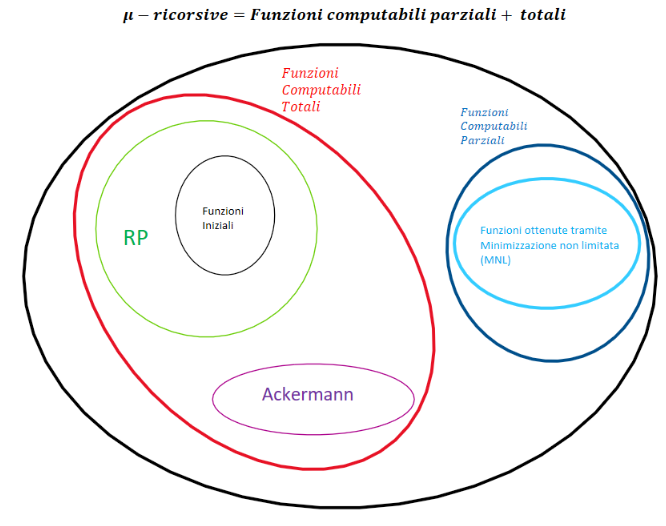
\includegraphics[width=0.9\linewidth]{funzioni-computabili.png}
\end{center}
%%%%%%%%%%%%%%%%%%%%%%%%%%%%%%%%%%%%%%%%%%%%%%%%%%%%%%%%%%%%%%%%%%%%%%%%%%%%%%%%%%%%%%%%%%%%%%%%%%%%%%
%%%%%%%%%%%%%%%%%%%%%%%%%%%%%%%%%%%%%%%%%%%%%%%%%%%%%%%%%%%%%%%%%%%%%%%%%%%%%%%%%%%%%%%%%%%%%%%%%%%%%%
\section{Decidibilità}
\begin{tikzpicture}[
		level 1/.style={
				sibling distance=40mm,
				level distance=20mm,
				every node/.append style={font=\small} % qui riduco il font dei figli
			},
		every node/.style={
				rectangle, draw, rounded corners,
				align=center,
				top color=blue!20,
				bottom color=blue!10
			}
	]
	\node {Linguaggio}
	child {node {Decidibile}}
	child {node {Semidecidibile}}
	child {node {Indecidibile}};
\end{tikzpicture}\newline \newline
Come provare che un linguaggio è decidibile, semidecidibile o indecidibile?
\begin{itemize}
	\item $L$ è decidibile: dimostrazione per costruzione
	\item $L$ è semidecidibile: dimostrazione per costruzione
	\item $L$ è indecidibile: dimostrazione per assurdo + riduzione ad un problema che sappiamo essere indecidibile (es: Teorema dell'arresto) oppure Teorema di Rice
\end{itemize}
\begin{definition}[Codifica di una MdT] La notazione $R(M)$ indica la codifica di una macchina. Spesso utilizzata nelle dimostrazioni.
\end{definition}
\subsection{Decidibilità}
Un linguaggio $L$ è \textbf{decidibile} se $\exists$ una MdT $M$ tale che, per ogni stringa $w\in \Sigma^*$ in input:
\begin{itemize}
	\item Se $w \in L \implies$ M si ferma (accettando $w$) nello stato $q_{accept}$; Quindi accetta la stringa.
	\item Se $w \notin L \implies$ M si ferma (rifiutando $w$) nello stato $q_{reject}$; Quindi rifiuta la stringa.
\end{itemize}
Notare che la macchina si ferma sempre. In questo caso si dice che la macchina "decide" $L$.
\begin{definition}[Enumeratore]
	Un \textcolor{red}{enumeratore} è una MdT che genera tutte le stringhe del linguaggio (separandole con il simbolo "$\#$"),
	una dopo l'altra, senza ricevere nessun input. Infatti, la macchina $E$ inizia a lavorare su nastro vuoto (input vuoto). \newline \newline
	Funzionamento:
	\begin{enumerate}
		\item L'enumeratore viene eseguito inizialmente su nastro vuoto (nessun input)
		\item Genera la stringa scrivendola sul nastro
		\item Quando ha terminato di scrivere la stringa, la invia al dispostivo di output (stampante)
		\item Torna al passo 2
	\end{enumerate}
\end{definition}
\begin{definition}[Funzione caratteristica]
	Sia $L$ un linguaggio su $\Sigma^*$. La \textcolor{red}{funzione caratteristica} di $L$, dato in input una stringa $w$, restituisce $1$ se la stringa appartiene al linguaggio,
	$0$ altrimenti:
	\[
		\mbox{\Large$\chi$}_L (w) =
		\begin{cases}
			\text{1} & \text{se } w \in L    \\
			\text{0} & \text{se } w \notin L
		\end{cases}
	\]
	La funzione caratteristica è una MdT.
\end{definition}
\begin{theorem}{2.1.1}
	SSe $L$ è decidibile $\implies L$ è enumerabile.
	\footnotesize % riduce la dimensione del font
	\begin{ragionamento}
		Per dimostrarlo, utilizzo la dimostrazione per costruzione.
	\end{ragionamento}
	\begin{proof}
		\begin{align*}
			L \text{ è decidibile} \tag*{(ipotesi)}
		\end{align*}
		\begin{align*}
			L \text{ è enumerabile} \tag*{(tesi)}
		\end{align*}
		Sia $L$ il linguaggio su $\Sigma^*$. Per ipotesi, $L$ è decidibile quindi $\exists$ una MdT $M$ che decide $L$.
		Costruisco un MdT $E$ che enumera $L$ come segue. \\ \\
		$E$ non ha nessun input ma $\forall{w_i} \in \Sigma^*$:
		\begin{enumerate}
			\item Esegue $M$ su $w_i$:
			      \begin{itemize}
				      \item Se $M$ accetta ($w_i \in L$) allora $E$ scrive $w_i$
				      \item Se $M$ rifiuta ($w_i \notin L$) allora $E$ non scrive $w_i$
			      \end{itemize}
		\end{enumerate}
		Ho costruito un enumeratore per $L$. Pertanto $L$ è enumerabile.
	\end{proof}
\end{theorem}
\begin{theorem}{2.1.2}
	d$L$ è decidibile $\iff L$ è enumerabile$\;\wedge\; \overline{L}$ è enumerabile.
	\footnotesize % riduce la dimensione del font
	\begin{ragionamento}
		$\overline{L}$ è enumerabile vuol dire che una MdT scrive tutte le stringhe $\notin L$
	\end{ragionamento}
\end{theorem}
\begin{theorem}{2.1.3}
	a$L$ è decidibile $\iff \mbox{\Large$\chi$}_L$ è una funzione computabile.
	\footnotesize % riduce la dimensione del font
	\begin{ragionamento}
		$\mbox{\Large$\chi$}_L$ funzione computabile vuol dire che $\exists$ una MdT, dato in input $w$, restituisce:
		\[
			\mbox{\Large$\chi$}_L(w) =
			\begin{cases}
				1 & \text{se } w \in L,    \\
				0 & \text{se } w \notin L.
			\end{cases}
		\]
	\end{ragionamento}
\end{theorem}
\begin{theorem}{2.1.4}
	SSe $L$ è decidibile $\implies L$ è semidecidibile.
\end{theorem}
Questa dimostrazione fa riferimento ad un automa a stati finiti deterministico (DFA). Lo stesso quesito per una MdT non è decidibile (vedi esercizio 2.2).
Lo scopo è mostrare come funziona la dimostrazione per costruzione.
\begin{esercizio}[Esercizio 1.1]
	\footnotesize % riduce la dimensione del font
	Sia il linguaggio $L_{DFA} = \{(R(M), w) \mid M \text{ accetta } w\}$. Dimostrare che $L$ è decidibile.
	\begin{ragionamento}
		$L_{DFA}$ è l'insieme delle codifiche di automi a stati finiti deterministici che accettano $w$. Ovvero, siano $M_1$,$M_2$,$M_3$ tre DFA:
		\begin{itemize}
			\item $M_1$ accetta $w$, allora $R(M_1) \in L_{DFA}$
			\item $M_2$ rifiuta $w$, allora $R(M_2) \notin L_{DFA}$
			\item $M_3$ accetta $w$, allora $R(M_3) \in L_{DFA}$
		\end{itemize}
		Quindi \(L_{DFA}=\{R(M_1),R(M_3)\}\) \newline
		**utilizzo dimostrazione per costruzione.
	\end{ragionamento}
	\begin{proof}
		\begin{align*}
			L_{DFA} = \{(R(M), w) \mid M \text{ accetta } w\} \tag*{(ipotesi)}
		\end{align*}
		\begin{align*}
			L_{DFA} \text{è decidibile} \tag*{(tesi)}
		\end{align*}
		Sapendo che per ipotesi $L_{DFA} = \{(R(M), w) \mid M \text{ accetta } w\}$, allora costruisco una MdT $N$ che decide $L_{DFA}$.
		Dato in input $(R(M),w)$, dove $R(M)$ è la codifica di un DFA arbitrario e $w$ una stringa:
		\begin{enumerate}
			\item Controlla che $R(M)$ sia una codifica valida e che $w$ sia una stringa, altrimenti rifiuta.
			\item Simula $M$ su input $w$.
			\item Se la simulazione termina:
			      \begin{itemize}
				      \item in uno stato accettante $\implies N$ termina accettando $R(M)$; \\ Quindi $R(M) \in L_{DFA}$
				      \item in uno stato di rifiuto $\implies N$ termina rifiutando $R(M)$; \\ Quindi $R(M) \notin L_{DFA}$
			      \end{itemize}
		\end{enumerate}
		Ho costruito una macchina $N$ in grado di decidere $L_{DFA}$; Inoltre, poichè un DFA ha
		un numero di stati finiti e la stringa $w$ è finita, la simulazione termina in uno stato finale
		(accettante o di rifiuto), garantendo che anche $N$ si fermi sempre accettando o rifiutando l'input.
		Pertanto, si dimostra che $L_{DFA}$ è decidibile.
	\end{proof}
\end{esercizio}
%%%%%%%%%%%%%%%%%%%%%%%%%%%%%%%%%%%%%%%%%%%%%%%%%%%%%%%%%%%%%%%%%%%%%%%%%%%%%%%%
\subsection{Semidecidibilità}
Un linguaggio $L$ è \textbf{semidecidibile} se $\exists$ una MdT $M$ tale che, per ogni stringa $w\in \Sigma^*$ in input:
\begin{itemize}
	\item Se $w \in L \implies$ M si ferma (accettando $w$) nello stato $q_{accept}$; Quindi accetta la stringa.
	\item Se $w \notin L \implies$ M va in loop, non fermandosi mai.
\end{itemize}
Notare che la macchina \underline{non} si ferma sempre. In questo caso si dice che la macchina "riconosce" $L$.
\begin{theorem}{2.2.1}
	s$L$ è enumerabile $\iff L$ è semidecidibile.
	\footnotesize % riduce la dimensione del font
	\begin{ragionamento}
		Se io ho un linguaggio $L$ e mi chiedono:
		\begin{itemize}
			\item Sia $L$ enumerabile, è anche semidecidibile? (sempre vero)
			\item Sia $L$ semidecidibile, è anche enumerabile? (sempre vero)
		\end{itemize}
	\end{ragionamento}
	\begin{proof} ($\Longrightarrow$) \\
		\begin{align*}
			L \text{ è enumerabile} \tag*{(ipotesi)}
		\end{align*}
		\begin{align*}
			L \text{ è semidecidibile} \tag*{(tesi)}
		\end{align*}
		Per ipotesi, $\exists$ una MdT $E$ che enumera $L$. Costruisco un algoritmo di semidecisione $M$ per $L$ con il seguente funzionamento. \\ \\
		$M$ su input $w$:
		\begin{enumerate}
			\item Esegue $E$ e osserva le stringhe che esso stampa. Per ogni nuova stringa $s_i$ stampata da $E$: \\
			      $M$ confronta $w$ con $s_i$:
			      \begin{itemize}
				      \item Se $w=s_i$, allora $M$ accetta $w$.
			      \end{itemize}
		\end{enumerate}
		Se $w$ non appare mai tra le stringhe prodotte da $E$, $M$ non si ferma (continuerà a confrontare ogni stringa stampata da $E$). \\
		Ho costruito un algoritmo di semidecidibile per $L$, pertanto $L$ è semidecidibile.
	\end{proof}
	\textit{Nota per non confondersi: durante la costruzione di un algoritmo semidecidibile, specifica \textcolor{red}{solo} il comportamento di $M$ nel caso di $w \in L$, ma non
		nel caso in cui $w \notin L$. Perchè essendo $M$ semidecidibile, non importa specificarlo e potresti confonderti. Nel caso puoi menzionare che
		M non si ferma ma non andare nello specifico.} \\
	$\rule{\linewidth}{0.3pt}$  % linea orizzontale lunga quanto la pagina, spessore 0.4pt$
	\begin{proof} ($\Longleftarrow$) \\
		\begin{align*}
			L \text{ è semidecidibile} \tag*{(ipotesi)}
		\end{align*}
		\begin{align*}
			L \text{ è enumerabile} \tag*{(tesi)}
		\end{align*}
		Per ipotesi, $L$ è semidecidibile quindi $\exists$ una MdT $M$ che riconosce (semidecide) $L$.
		Costruisco un algoritmo di enumerazione $E$ per $L$ con il seguente funzionamento. \\
		\textcolor{red}{a) Versione con MdT deterministica} \\
		In questo caso si utilizza la tecnica di Dovetailing per Macchine di Turing. \\
		Ricordiamoci che $M$ è la MdT deterministica che semidecide $L$ dove: \\
		$M$ su input $w$, se $w \in L \implies M$ accetta. (non specifico nel caso di $w \notin L$, perchè $M$ può non terminare essendo semidecidibile). \\
		Costruisco un \textcolor{green!60!black}{\underline{\textbf{enumeratore $E$ deterministico}}} come segue. \\ \\
		$E$ non ha nessun input ma per ogni passo $i$:
		\begin{itemize}
			\item passo $i=1$:
			      \begin{enumerate}
				      \item $E$ simula $M$ su $w_1$ per $1$ passo (cioè $M$ effettua $1$ transizione su $w_1$)
				      \item Se $M$ accetta, $E$ stampa $w_1$
			      \end{enumerate}
			\item passo $i=2$:
			      \begin{enumerate}
				      \item $E$ simula $M$ su $w_1$ per $2$ passi (cioè $M$ effettua $2$ transizioni su $w_1$, ripartendo dallo stato iniziale)
				      \item Se $M$ accetta, $E$ stampa $w_1$
				      \item $E$ simula $M$ su $w_2$ per $2$ passi (cioè $M$ effettua $2$ transizioni su $w_2$)
				      \item Se $M$ accetta, $E$ stampa $w_2$
			      \end{enumerate}
			\item passo $i=3$:
			      \begin{enumerate}
				      \item $E$ simula $M$ su $w_1$ per $3$ passi (cioè $M$ effettua $3$ transizioni su $w_1$, ripartendo dallo stato iniziale)
				      \item Se $M$ accetta, $E$ stampa $w_1$
				      \item $E$ simula $M$ su $w_2$ per $3$ passi (cioè $M$ effettua $3$ transizioni su $w_2$, ripartendo dallo stato iniziale)
				      \item Se $M$ accetta, $E$ stampa $w_2$
				      \item $E$ simula $M$ su $w_3$ per $3$ passi (cioè $M$ effettua $3$ transizioni su $w_3$)
				      \item Se $M$ accetta, $E$ stampa $w_3$
			      \end{enumerate}
			\item passo $i=4$:
			      \begin{enumerate}
				      \item $E$ simula $M$ su $w_1$ per $4$ passi (cioè $M$ effettua $4$ transizioni su $w_1$, ripartendo dallo stato iniziale)
				      \item Se $M$ accetta, $E$ stampa $w_1$ \\ \\
				            \textit{CONTA CHE $w_2$ È GIÀ STATA ACCETTATA NEI PASSI PRECEDENTI QUINDI QUI NON C'È BISOGNO DI SCRIVERLA} \\
				      \item $E$ simula $M$ su $w_3$ per $4$ passi (cioè $M$ effettua $4$ transizioni su $w_3$, ripartendo dallo stato iniziale)
				      \item Se $M$ accetta, $E$ stampa $w_3$
				      \item $E$ simula $M$ su $w_4$ per $4$ passi (cioè $M$ effettua $4$ transizioni su $w_4$)
				      \item Se $M$ accetta, $E$ stampa $w_4$
			      \end{enumerate}
			\item $\dots$ (iterazioni successive)
		\end{itemize}
		È ovvio che con questo metodo $E$ non rimane mai bloccata perchè $M$ non si blocca su nessuna stringa $w_i$ perchè al $i$-esimo passo, $M$ esegue sulla stringa $i$ transizioni\footnote{a seconda
			del passo di $E$} (che sono finite\footnote{quindi $M$ si ferma per certo su $w_i$ dopo aver fatto $i$ transizioni}). \\ \\
		\textbf{Dopo aver compreso il meccanismo di Dovetailing per costruire un enumeratore tramite MdT deterministiche semidecidibili, posso riassumerlo così:} \\
		$E$ non ha nessun input: \\
		Ripeti quanto segue per $i=1,2,3,\dots$ passi
		\begin{enumerate}
			\item Simula $M$ su ogni input $w_1,w_2,...,w_i$ per $i$ passi
			\item Se una qualsiasi simulazione accetta, $E$ stampa la corrispondente stringa accettata.
		\end{enumerate}
		\underline{Conclusione:} Ho costruito un enumeratore $E$ deterministico che stampa tutte e solo le stringhe di $L$. Pertanto $L$ è enumerabile. \\ \\
		\textcolor{red}{b) Versione con MdT non deterministica} \\
		In questo caso si utilizza la seguente tecnica: Costruisco un enumeratore non deterministico che simula una mdt M det?
		Ricordiamoci che $M$ è la MdT deterministica che semidecide $L$ dove: \\
		$M$ su input $w$, se $w \in L \implies M$ accetta. (non specifico nel caso di $w \notin L$, perchè $M$ può non terminare essendo semidecidibile). \\
		Costruisco un \textcolor{green!60!black}{\underline{\textbf{enumeratore $E$ non deterministico}}} come segue. \\ \\
		$E$ non ha nessun input:
		\begin{enumerate}
			\item $E$ indovina\footnote{
				      Con "indovinare" si intende che $E$ eslora diversi rami contemporaneamente; Ogni ramo $i$ è indipendente e sceglie una stringa $w_i$:
				      \begin{align*}
					      Ramo_1 & : w_1 \rightarrow M(w_1) \\
					      Ramo_2 & : w_2 \rightarrow M(w_2) \\
					      Ramo_3 & : w_3 \rightarrow M(w_3) \\
					             & \vdots                   \\
					      Ramo_i & : w_i \rightarrow M(w_i)
				      \end{align*}
				      Quindi, è come se ci fossero tante $M$ parallele che si eseguono, ciasucuna su input diverso $w_i$. Inoltre, se $M$ va in loop su una $w$ (ramo), gli altri rami non
				      rimangono bloccati quindi segue che $E$ non rimane bloccata. Questo garantisce che, se almeno un ramo termina con accettazione, allora l'enumeratore $E$ stampa la stringa
				      accettata da $M$.
			      } una stringa $w$.
			\item $E$ simula $M$ su $w$:
			      \begin{itemize}
				      \item se $M$ accetta $w$, allora $E$ stampa la stringa
			      \end{itemize}
		\end{enumerate}
		\underline{Conclusione:} Ho costruito un enumeratore $E$ non deterministico che stampa tutte e sole le stringhe di $L$. Pertanto $L$ è enumerabile.
	\end{proof}
\end{theorem}
\begin{theorem}{2.2.2}
	S$L$ è semidecidibile$\;\wedge\; \overline{L}$ è semidecidibile $\implies L$ decidibile.
\end{theorem}
\begin{theorem}{2.2.3}
	S$L$ è semidecidibile$\;\wedge\; \overline{L}$ non è semidecidibile $\implies L$ indecidibile.
\end{theorem}

%%%%%%%%%%%%%%%%%%%%%%%%%%%%%%%%%%%%%%%%%%%%%%%%%%%%%%%%%%%%%%%%%%%%%%%%%%%%%%%%
\subsection{Indecidibilità}
Un linguaggio $L$ è indecidibile quando $\nexists$ una MdT in grado di fermarsi sempre accettando o rifiutando l'input. Ciò vuol dire che:
\begin{itemize}
	\item $L$ è indecidibile e anche semidecidibile
	\item $L$ è indecidibile ma non semidecidibile
\end{itemize}
Pertanto, quando viene richiesto di dimostrare l'indecidibilità di un linguaggio:
\begin{itemize}
	\item Se sospetto che $L$ possa essere indecidibile $+$ semidecidibile, allora:
	      \begin{enumerate}
		      \item Applico la dimostrazione per costruzione;

		            cioè, costruisco una MdT che riconosce\footnote{Turing-reconizable: MdT si ferma accettando le stringhe che appartengono al linguaggio e va in loop
			            per quelle che non appartengono.} il linguaggio.
		      \item Effettuo la riduzione ad un linguaggio noto indecidibile.
	      \end{enumerate}
	      Nel primo punto dimostro la semidecidibilità di $L$ e nel secondo la indecidibilità.
	\item Se sospetto che il linguaggio è indecidibile ma non semidecidibile, allora posso considerare una di queste tecniche:
	      \begin{center}
		      \begin{tikzpicture}[
				      level 1/.style={
						      sibling distance=30mm,
						      level distance=20mm,
						      every node/.append style={font=\small} % qui riduco il font dei figli
					      },
				      every node/.style={
						      rectangle, draw, rounded corners,
						      align=center,
						      top color=blue!20,
						      bottom color=blue!10
					      }
			      ]
			      \node {Dimostrare indecidibilità}
			      child {node {dim assurdo \\ + riduzione}}
			      child {node {riduzione diretta}}
			      child {node {teorema di Rice}}
			      child {node {diagonalizzazione}};
		      \end{tikzpicture}
	      \end{center}

	      \begin{itemize}
		      \item dimostrazione per assurdo + effettuo la riduzione ad un linguaggio noto indecidibile
		      \item riduzione diretta
		      \item uso il Teorema di Rice
		      \item applico la diagonalizzazione
	      \end{itemize}
\end{itemize}

\subsection{Proprietà di Chiusura dei linguaggi}
\begin{center}
	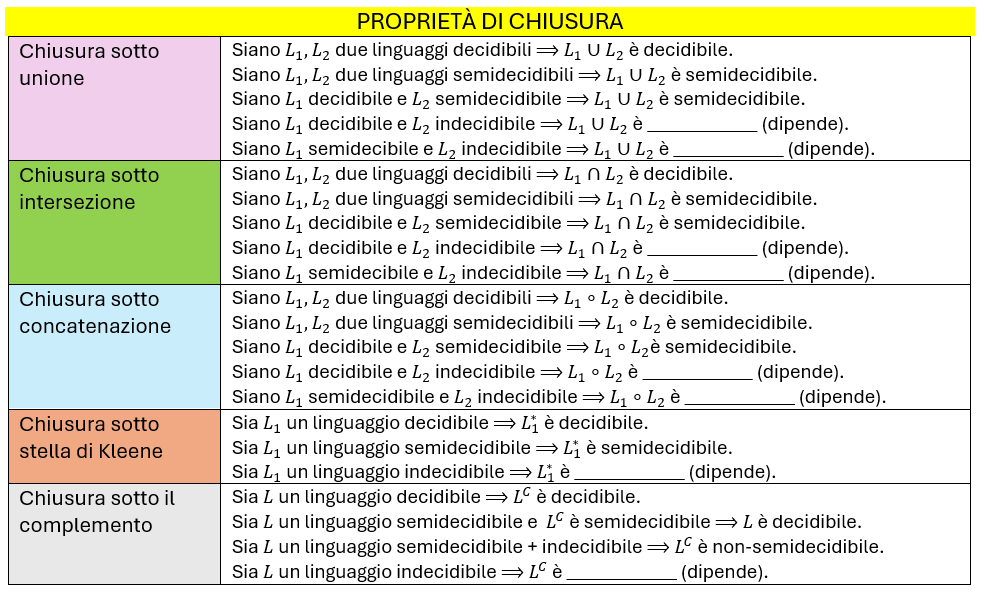
\includegraphics[width=0.9\linewidth]{chiusura-linguaggi.png}
\end{center}

\subsection{Esercizi}
\begin{theorem}{}
	SSia il linguaggio $L = \{(R(M), w) \mid M \text{ accetta } w\}$. Dimostrare che $L$ è semidecidibile ma anche indecidibile.
\end{theorem}
\begin{esercizio}[Esercizio 2.1]
	\footnotesize % riduce la dimensione del font
	Sia il linguaggio $L_1 = \{(R(M), w) \mid M \text{ accetta } w\}$. Dimostrare che $L$ è semidecidibile.
	\begin{ragionamento}
		$L_1$ è l'insieme delle codifiche di MdT che accettano $w$. Ovvero, siano $M_1$,$M_2$,$M_3$ tre MdT:
		\begin{itemize}
			\item $M_1$ accetta $w$, allora $R(M_1) \in L_1$
			\item $M_2$ rifiuta $w$, allora $R(M_2) \notin L_1$
			\item $M_3$ accetta $w$, allora $R(M_3) \in L_1$
		\end{itemize}
		Quindi \(L_1=\{R(M_1),R(M_3)\}\)  \\
		Dato che devo dimostrare la semidecidibilità di $L_1$, costruisco una MdT che riconosce il linguaggio.
	\end{ragionamento}
	\begin{proof}
		\begin{align*}
			L_1 = \{(R(M), w) \mid M \text{ accetta } w\} \tag*{(ipotesi)}
		\end{align*}
		\begin{align*}
			L_1 \text{ è semidecidibile} \tag*{(tesi)}
		\end{align*}
		Costruisco una MdT $N$ che riconosce $L_1$.
		Dato in input $(R(M),w)$, dove $R(M)$ è la codifica di una MdT arbitraria e $w$ una stringa, la MdT $N$ si comporta come segue:
		\begin{enumerate}
			\item Controlla che $R(M)$ sia una codifica valida e che $w$ sia una stringa, altrimenti rifiuta.
			\item Simula $M$ su input $w$.
			\item Se la simulazione termina:
			      \begin{itemize}
				      \item in uno stato accettante $\implies N$ termina accettando $R(M)$; \\ Quindi $R(M) \in L_1$
				      \item in uno stato di rifiuto $\implies N$ termina rifiutando $R(M)$; \\ Quindi $R(M) \notin L_1$
			      \end{itemize}
		\end{enumerate}
		Notare che la macchina $N$ va in loop sull'input $(R(M),w)$ se $M$ va in loop su $w$. \\
		Un decisore deve \underline{sempre} fermarsi (in ogni caso), ma qui, se $M$ va in loop su $w$, $N$ non si fermerà mai.
		Questo rende $N$ un riconoscitore e non un decisore. \\
		Ho dimostrato che $L_1$ è semidecidibile costruendo la MdT $N$ che riconosce tale linguaggio.
		Pertanto, si dimostra che $L_1$ è semidecidibile.
	\end{proof}
\end{esercizio}

\begin{esercizio}[Esercizio 2.2]
	\footnotesize % riduce la dimensione del font
	Sia il linguaggio $L_1 = \{(R(M), w) \mid M \text{ accetta } w\}$. Dimostrare che $L$ è indecidibile.
	\begin{ragionamento}
		Per dimostrarlo, applico:
		\begin{itemize}
			\item Dim per assurdo (suppongo per assurdo (nego la tesi) per poi ottenere una contraddizione, che rende falsa l'assunzione fatta)
		\end{itemize}
	\end{ragionamento}
	\begin{proof}
		\begin{align*}
			L_1 = \{(R(M), w) \mid M \text{ accetta } w\} \tag*{(ipotesi)}
		\end{align*}
		\begin{align*}
			L_1 \text{ è indecidibile} \tag*{(tesi)}
		\end{align*}
		Per applicare la dimostrazione per assurdo nego la tesi, quindi suppongo per assurdo che $L_1$ sia decidibile.
		Sapendo che per ipotesi (la mia per assurdo, non quella del teorema) $L_1$ è decidibile, allora $\exists$ una MdT $N$ che decide $L_1$ con il seguente funzionamento:
		\[
			N(R(M),w) =
			\begin{cases}
				\text{accept} & \text{se } M \text{ accetta } w     \\
				\text{reject} & \text{se } M \text{ non accetta } w
			\end{cases}
		\]
		Con "non accetta" si intende che $M$ potrebbe rifiutare $w$ oppure andare in loop.\\
		Dato in input $(R(M),w)$ alla MdT $N$, dove $R(M)$ è la codifica di una MdT arbitraria e $w$ una stringa:
		\begin{enumerate}
			\item $N$ controlla che $R(M)$ sia una codifica valida e che $w$ sia una stringa, altrimenti rifiuta.
			\item Simula $M$ su input $w$.
			\item Se la simulazione termina:
			      \begin{itemize}
				      \item in uno stato accettante $\implies N$ termina accettando $R(M)$; \\ Quindi $R(M) \in L_1$
				      \item in uno stato di rifiuto/va in loop $\implies N$ termina rifiutando $R(M)$; \\ Quindi $R(M) \notin L_1$
			      \end{itemize}
		\end{enumerate}
		Adesso costruisco una nuova MdT $D$ con $N$ come subroutine. $D$ chiama $N$ per determinare cosa fa $M$ quando l'input per $M$ è la sua
		stessa codifica (e non la stringa $w$). Il comportamento di $D$ è l'opposto di $N$, ovvero:
		\[
			D(R(M)) =
			\begin{cases}
				\text{accept} & \text{se } M \text{ non accetta } R(M) \\
				\text{reject} & \text{se } M \text{  accetta } R(M)
			\end{cases}
		\]
		Funzionamento di $D$:
		\begin{enumerate}
			\item Esegue $N$ su input $(R(M),R(M))$ dove $R(M)$ è la codifica della MdT M:
			      \begin{itemize}
				      \item Se $N$ si ferma accettando $\implies$ $D$ rifiuta.\\
				            (ricorda che se $N$ accetta allora vuol dire che $M$ ha accettato $R(M)$)
				      \item Se $N$ si ferma rifiutando $\implies$ $D$ accetta. \\
				            (ricorda che se $N$ rifiuta allora vuol dire che $M$ non ha accettato $R(M)$)
			      \end{itemize}
		\end{enumerate}
		Cosa succederebbe se fornissimo alla MdT $D$ la propria codifica come input? Otterrei:
		\[
			D(R(D)) =
			\begin{cases}
				\text{accept} & \text{se } D \text{ non accetta } R(D) \\
				\text{reject} & \text{se } D \text{  accetta } R(D)
			\end{cases}
		\]
		che è una contraddizione.\\
		\textbf{Conclusione:} Poiché abbiamo ottenuto una contraddizione ($D$ rifiuta $R(D)$ quando $D$ accetta $R(D)$), l’ipotesi che $L_1$ sia decidibile è falsa. Pertanto, $L_1$ è indecidibile.
	\end{proof}
\end{esercizio}

\begin{theorem}{}
	SSia il linguaggio $L = \{(R(M), w) \mid M \text{ accetta } w\}$. Dimostrare che $\overline{L}$ non è semidecidibile.
\end{theorem}
\begin{esercizio}[Esercizio 2.3]
	\footnotesize % riduce la dimensione del font
	Sia il linguaggio $L_1 = \{(R(M), w) \mid M \text{ accetta } w\}$. Dimostrare che $\overline{L_1}$ non è semidecidibile.
	\begin{ragionamento}
		Devo dimostrare che $\overline{L_1}=\{(R(M), w) \mid M \text{ non accetta } w\}$ non è semidecidibile, ovvero che $\nexists$ una MdT in grado
		di riconoscere $\overline{L_1}$. Procedo per assurdo.
	\end{ragionamento}
	\begin{proof}
		\begin{align*}
			L_1 = \{(R(M), w) \mid M \text{ accetta } w\} \tag*{(ipotesi)}
		\end{align*}
		\begin{align*}
			\overline{L_1} \text{ non è semidecidibile} \tag*{(tesi)}
		\end{align*}

		Sappiamo che $L_1$ è un linguaggio semidecidibile (esercizio 2.1). \\
		Suppongo per assurdo che anche $\overline{L_1}$ sia semidecidibile (nego la tesi, ipotesi per assurdo).
		Dato che $L_1, \overline{L_1}$ sono entrambi semidecidibili $\implies$ per definizione, $L_1$ è decidibile. Ma questo è assurdo perchè abbiamo dimostrato
		che $L_1$ è indecidibile (esercizio 2.2). Ciò porta ad una contraddizione e l'ipotesi che $\overline{L_1}$ sia semidecidibile è falsa.
		Pertanto, $\overline{L_1}$ è non semidecidibile.

	\end{proof}
\end{esercizio}
\break
\subsection{Famosi problemi indecidibili}
\subsubsection{Halting Problem}
\begin{definition}(Problema dell'arresto)
	Esiste una MdT $H$ che preso in input $(M,w)$, termina dicendo:
	\begin{itemize}
		\item Sì, se $M$ termina su $w$
		\item No, se $M$ va in loop su $w$
	\end{itemize}
	Tale macchina esiste? No.
\end{definition}
\begin{definition}(Linguaggio Halting Problem) Sia $\mathcal{L}_{\text{Halt}}$ il linguaggio del problema dell'arresto definito come segue:
	\begin{align*}
		\mathcal{L}_{\text{Halt}} = \{(R(M),w) \mid M \text{ termina su } w\}
	\end{align*}
	Notare che $\mathcal{L}_{\text{Halt}}$ è semidecidibile, ovvero $\exists$ una MdT $N$ che dato in input $(R(M),w)$:
	\begin{itemize}
		\item Se $M$ termina su $w$, allora $N$ accetta \\ (Se $M$ termina su $w \implies (R(M),w) \in \mathcal{L}_{\text{Halt}}$)\footnote{Ho scritto
			      "$M$ termina su $w$" e non "$w \in L(M)$" poichè si sta parlando di terminare su $w$ e non accettare $w$. La dicitura
			      classica $w \in L(M)$ si scrive solo quando $M$ accetta $w$.}.
		\item Se $M$ non termina su $w$, allora $N$ va in loop
	\end{itemize}
	*Attenzione: "$M$ termina su $w$" e non dice "$M$ accetta $w$", che sono due cose differenti.
	Se $M$ termina su $w$, allora $N$ accetta; ovvero l'importante è che $M$ termini su $w$, che sia in uno stato accettante o di rifiuto. (Quindi non ci interessa
	se $M$ accetta o rifiuta $w$, quello che ci interessa è che $M$ si fermi su $w$.) \\ \\
	Pertanto, $\exists$ una MdT che riconosce (ma non decide) $\mathcal{L}_{\text{Halt}}$.
\end{definition}

\begin{osservazioni}[Osservazione]
	\footnotesize % riduce la dimensione del font
	Il problema dell'arresto (o, equivalentemente, il linguaggio
	$\mathcal{L}_{\text{Halt}}$) è \textbf{indecidibile}, cioè non esiste una MdT che
	termina sempre dando la risposta corretta.
	Tuttavia, $\mathcal{L}_{\text{Halt}}$ è \textbf{semidecidibile}: esiste infatti una MdT universale che, dato in input
	$(R(M),w)$, termina accettando se $M$ termina su $w$, mentre può non
	terminare se $M$ non termina su $w$.
\end{osservazioni}

Il problema dell'arresto è semidecidibile + indecidibile, oppure, equivalentemente scrivo:
\begin{align*}
	\textcolor{red}{\mathcal{L}_{\text{Halt}} \text{ è semidecidibile ma non decidibile}}
\end{align*}

\begin{theorem}{Halting Problem (2.4.1)}
	IIl problema dell'arresto è indecidibile. \\
	$\mathcal{L}_{\text{Halt}} = \{(R(M),w) \mid M \text{ termina su } w\}$ è indecidibile.
	\footnotesize % riduce la dimensione del font
	\begin{proof}
		\begin{align*}
			\mathcal{L}_{\text{Halt}} = \{(R(M),w) \mid M \text{ termina su } w\} \tag*{(ipotesi)}
		\end{align*}
		\begin{align*}
			\mathcal{L}_{\text{Halt}} \text{ è indecidibile} \tag*{(tesi)}
		\end{align*}
		Suppongo per assurdo che il problema dell'arresto sia decidibile (ipotesi per assurdo, nego la tesi).
		Quindi, per ipotesi, $\exists$ una MdT $H$ che risolve il problema dell'arresto. \\
		$H$ su input ($R(M),w$) dove $R(M)$ è la codifica di una MdT arbitraria e $w$ una stringa:
		\begin{itemize}
			\item Se $M$ termina su $w$, allora $H$ accetta
			\item Se $M$ non termina su $w$, allora $H$ rifiuta
		\end{itemize}
		Modifico la MdT $H$ per costruire $H'$ con il seguente
		comportamento.
		\[
			H'(R(M),w) =
			\begin{cases}
				\text{loop}   & \text{se } M \text{ termina su } w      \\
				\text{reject} & \text{se } M \text{  non termina su } w
			\end{cases}
		\]
		$H'$ su input ($R(M),w$):
		\begin{itemize}
			\item Se $M$ termina su $w$, allora $H'$ va in loop
			\item Se $M$ non termina su $w$, allora $H'$ rifiuta
		\end{itemize}
		Adesso costruisco un'altra MdT $D$ (che prende in input solo la codifica di una macchina)\footnote{invece dell'input
			($R(M),w$), prende in input ($R(M)$)}
		combinando $H'$ con una procedura.
		\[
			D(R(M)) =
			\begin{cases}
				\text{loop}   & \text{se } M \text{ termina su } R(M)      \\
				\text{reject} & \text{se } M \text{  non termina su } R(M)
			\end{cases}
		\]
		La macchina $D$ su input ($R(M)$):
		\begin{enumerate}
			\item Controlla che $R(M)$ sia un codifica valida, altrimenti rifiuta
			\item Esegue varie transizioni che, a partire dall'input, produce la coppia ($R(M),R(M)$) \\
			      (legge la codifica della macchina in input e la copia come secondo argomento da fornire a $H'$)
			\item Esegue $H'$ sull'input ($R(M),R(M)$):
			      \begin{itemize}
				      \item Se $H'$ va in loop, allora anche $D$ va in loop \\
				            (ricorda che se $H'$ va in loop vuol dire che $M$ ha terminato su $R(M)$)
				      \item Se $H'$ rifiuta, allora $D$ rifiuta \\
				            (ricorda che se $H'$ rifiuta vuol dire che $M$ non ha mai terminato su $R(M)$)
			      \end{itemize}
		\end{enumerate}
		E adesso cosa succederebbe se fornissi alla MdT $D$ la propria codifica come input? Otterrei:
		\[
			D(R(D)) =
			\begin{cases}
				\text{loop}   & \text{se } D \text{ termina su } R(D)      \\
				\text{reject} & \text{se } D \text{  non termina su } R(D)
			\end{cases}
		\]
		una contraddizione. \\
		\textbf{Conclusione:} Poichè ho ottenuto una contraddizione ($D$ va in loop su $R(D)$ $\iff$ $D$ termina su $R(D)$), l'ipotesi
		che il problema dell'arresto sia decidibile è falsa. Pertanto, il problema dell'arresto è indecidibile (oppure scrivo:
		Pertanto, $\mathcal{L}_{\text{Halt}}$ è indecidibile).
	\end{proof}
\end{theorem}
\begin{theorem}{}
	I $\mathcal{L}_{\text{Halt}}$ è semidecidibile.
	$\overline{\mathcal{L}_{\text{Halt}}}$ non è semidecidibile.
	\footnotesize % riduce la dimensione del font
	\begin{proof}
		Sappiamo per definizione, che $\mathcal{L}_{\text{Halt}}$ è semidecidibile. \\
		Suppongo per assurdo che $\overline{\mathcal{L}_{\text{Halt}}}$ sia anch'esso semidecidibile. Dato che
		$\overline{\mathcal{L}_{\text{Halt}}}$,$\mathcal{L}_{\text{Halt}}$ sono entrambi semidecidibili $\implies$ per
		definizione, $\mathcal{L}_{\text{Halt}}$ è decidibile. Ma questo è assurdo perchè abbiamo dimostrato che
		$\mathcal{L}_{\text{Halt}}$ è indecidibile (teorema 2.4.1). Ciò porta ad una contraddizione e l'ipotesi che $\overline{\mathcal{L}_{\text{Halt}}}$
		sia semidecidibile è falsa. \\ Pertanto, $\overline{\mathcal{L}_{\text{Halt}}}$ è non semidecidibile.
	\end{proof}
\end{theorem}

\subsubsection{Problema del nastro vuoto}
\begin{definition}[Problema del nastro vuoto]
	Esiste una MdT $E$ che preso in input $R(M)$, termina dicendo:
	\begin{itemize}
		\item Sì, se $M$ termina su nastro vuoto
		\item No, se $M$ non termina su nastro vuoto
	\end{itemize}
	Tale macchina esiste? No. \\
	\footnotesize % riduce la dimensione del font
	*Attenzione: "termina su nastro vuoto" significa "termina quando parte su nastro vuoto".
\end{definition}
\begin{definition}[Linguaggio Blank-Tape Halting Problem]
	Sia $\mathcal{L}_{\text{Blank-Tape}}$ il linguaggio del problema del nastro vuoto definito come segue:
	\begin{align*}
		\mathcal{L}_{\text{Blank-Tape}} = \{R(M) \mid M \text{ termina su nastro vuoto}\}
	\end{align*}
	Notare che $\mathcal{L}_{\text{Blank-Tape}}$ è semidecidibile.
\end{definition}
Quindi, il problema del nastro vuoto è semidecidibile + indecidibile, oppure, equivalentemente scrivo:
\begin{align*}
	\textcolor{red}{\mathcal{L}_{\text{Blank-Tape}} \text{ è semidecidibile ma non decidibile}}
\end{align*}


\begin{theorem}{Blank-Tape Halting Problem (versione A)}
	IIl problema del nastro vuoto è indecidibile. \\
	$\mathcal{L}_{\text{Blank-Tape}} = \{R(M) \mid M \text{ termina su nastro vuoto}\}$ è indecidibile.
	\footnotesize % riduce la dimensione del font
	\begin{ragionamento}
		Per dimostrarlo, uso la dim per assurdo e poi effettuo una riduzione da un problema noto indecidibile (es: problema dell'arresto) al mio (problema del nastro vuoto). \\
		Dato che sto ragionando per assurdo, non posso usare questa: se $A \leq_m B$ $\;\wedge\;$ $A$ è indecidibile $\implies$ $B$ è indecidibile (teorema 3.2); ma devo usare
		questa: se $A \leq_m B$ $\;\wedge\;$ $B$ è decidibile $\implies$ $A$ è decidibile (teorema 3.1); \\
		Quindi costruisco una riduzione del tipo: $\mathcal{L}_{\text{Halt}} \leq_m \mathcal{L}_{\text{Blank-Tape}}$.
	\end{ragionamento}
	\begin{proof}
		\begin{align*}
			\mathcal{L}_{\text{Blank-Tape}} = \{R(M) \mid M \text{ termina su nastro vuoto}\} \tag*{(ipotesi)}
		\end{align*}
		\begin{align*}
			\mathcal{L}_{\text{Blank-Tape}} \text{ è indecidibile} \tag*{(tesi)}
		\end{align*}
		Siano $\mathcal{L}_{\text{Halt}}$ , $\mathcal{L}_{\text{Blank-Tape}}$ due linguaggi su $\Sigma_H^*$, $\Sigma_B^*$ rispettivamente, dove:
		\begin{itemize}
			\item $\mathcal{L}_{\text{Halt}}$ è il linguaggio del problema dell'arresto
			\item $\mathcal{L}_{\text{Blank-Tape}}$ è il linguaggio del problema del nastro vuoto
		\end{itemize}
		\textcolor{red}{1. Ipotesi per assurdo} \\
		Suppongo per assurdo che $\mathcal{L}_{\text{Blank-Tape}}$ sia decidibile (ipotesi per assurdo). Quindi per ipotesi $\exists$ una MdT $E$
		che decide $\mathcal{L}_{\text{Blank-Tape}}$. Ovvero:
		\[
			E(R(M)) =
			\begin{cases}
				\text{accept} & \text{se } M \text{ termina su nastro vuoto}      \\
				\text{reject} & \text{se } M \text{  non termina su nastro vuoto}
			\end{cases}
		\]
		\textcolor{red}{2. Costruisco funzione di riduzione} \\
		Costruisco una funzione di riduzione $f: \Sigma_H^* \rightarrow \Sigma_B^*$ t.c. $\forall{w} \in \Sigma_H^*$:
		\begin{align*}
			w \in \mathcal{L}_{\text{Halt}} \iff f(w) \in \mathcal{L}_{\text{Blank-Tape}}
		\end{align*}
		Quindi, costrusco la funzione di riduzione (che sarebbe la MdT $R$):
		\begin{itemize}
			\item Se $w$ non è della forma $(R(M),w)$, pongo $f(w)=1$
			\item Se $w=(R(M),w)$, allora pongo $f(w)=R(M')$
		\end{itemize}
		Ovvero, il funzionamento della MdT $R$ è costruire una nuova macchina $M'$, praticamente il seguente:
		\begin{enumerate}
			\item $R$ riceve come input $w=(R(M),w)$ da $N$
			\item $R$ costruisce la nuova macchina $M'$ che ha questo comportamento:
			      \begin{enumerate}
				      \item $M'$ viene avviata su nastro vuoto (condizione del Blank-Tape Halting Problem)
				      \item $M'$ scrive $w$ sul nastro
				      \item $M'$ riporta la testina all'inizio del nastro
				      \item $M'$ esegue $M$ su $w$
			      \end{enumerate}
			\item $R$ genera l'output $R(M')$ (che è la nuova macchina costruita nel passo 2)
		\end{enumerate}
		\textcolor{red}{3. Costruisco MdT che decide il problema dell'arresto} \\
		Adesso, costrusco una MdT $N$ che decide $\mathcal{L}_{\text{Halt}}$:
		\begin{enumerate}
			\item $N$ su input $w \in \Sigma_H^*$ calcola $f(w) \in \Sigma_B^*$
			\item $N$ esegue $E$ su $f(w)$:
			      \begin{itemize}
				      \item Se $E$ accetta, allora $N$ accetta \\
				            (ricorda che se $E$ accetta, vuol dire che $M'$ ha terminato su nastro vuoto (se $M'$ termina su nastro vuoto, vuol
				            dire che $M$ ha terminato su $w$))
				            ovvero: Se $R(M') \in \mathcal{L}_{\text{Blank-Tape}}$, allora $(R(M),w) \in \mathcal{L}_{\text{Halt}}$ \\
				            ma è più corretto scrivere: \\
				            $w \in \mathcal{L}_{\text{Halt}} \iff  f(w) \in \mathcal{L}_{\text{Blank-Tape}}$
				      \item Se $E$ rifiuta, allora $N$ rifiuta \\
				            (ricorda che se $E$ rifiuta, vuol dire che $M'$ non ha terminato su nastro vuoto (se $M'$ non termina su nastro vuoto (loop), vuol
				            dire che $M$ non ha terminato su $w$ (loop))) \\
				            ovvero: Se $R(M') \notin \mathcal{L}_{\text{Blank-Tape}}$, allora $(R(M),w) \notin \mathcal{L}_{\text{Halt}}$ \\
				            ma è più corretto scrivere: \\
				            $w \notin \mathcal{L}_{\text{Halt}} \iff f(w) \notin \mathcal{L}_{\text{Blank-Tape}}$
			      \end{itemize}
		\end{enumerate}
		Quindi $N$ è un algoritmo di decisione per il problema dell'arresto che applica la funzione di riduzione per ogni input e sfrutta
		la MdT $E$ che decide $\mathcal{L}_{\text{Blank-Tape}}$ per decidere $\mathcal{L}_{\text{Halt}}$. Perchè alla fine $N$ si ferma
		accettando $w$ se e solo se $E$ si ferma accettando $f(w)$ oppure $N$ si ferma
		rifiutando $w$ se e solo se $E$ si ferma rifiutando $f(w)$. \\
		La costruzione e il funzionamento della MdT $N$ rende il problema dell'arresto decidibile. Ma questo è assurdo perchè sappiamo
		che il problema dell'arresto è indecidibile, quindi questo porta ad una contraddizione. Poichè ho ottenuto una contraddizione, l'ipotesi
		che il problema del nastro vuoto sia decidibile è falsa. Pertanto, il problema del nastro vuoto è indecidibile.
	\end{proof}
	Disegno: \\
	\begin{center}
		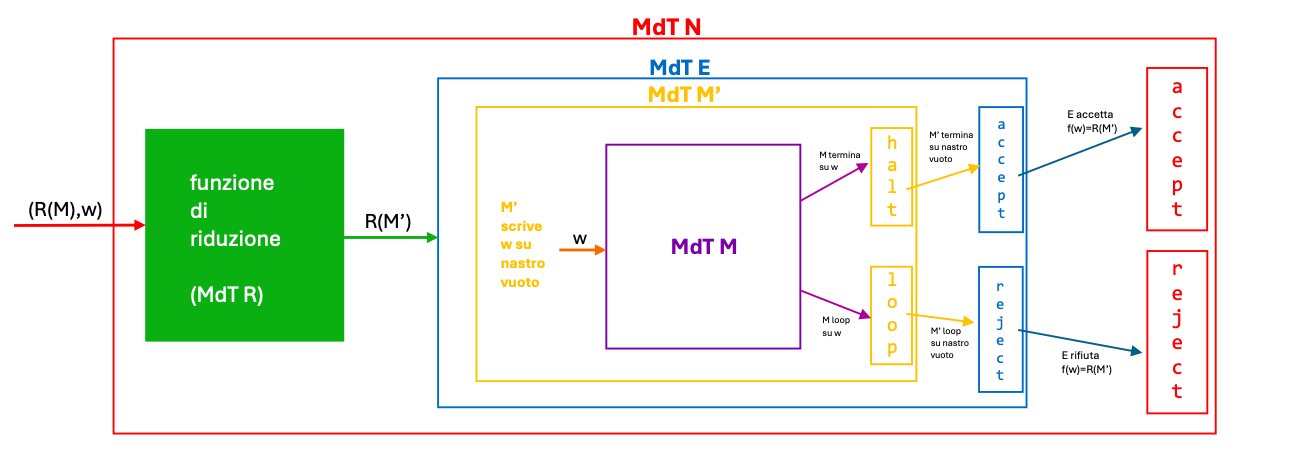
\includegraphics[width=0.9\linewidth]{BTHP.png}
	\end{center}
\end{theorem}

\begin{theorem}{Blank-Tape Halting Problem (versione B)}
	IIl problema del nastro vuoto è indecidibile. \\
	$\mathcal{L}_{\text{Blank-Tape}} = \{R(M) \mid M \text{ termina su nastro vuoto}\}$ è indecidibile.
	\footnotesize % riduce la dimensione del font
	\begin{ragionamento}
		Per dimostrarlo, \underline{non} uso la dim per assurdo ma effettuo \textbf{direttamente} una riduzione dal problema dell'arresto al mio. Ovvero,
		costruisco una riduzione del tipo: $\mathcal{L}_{\text{Halt}} \leq_m \mathcal{L}_{\text{Blank-Tape}}$. \\
		Uso solo la riduzione perchè "sfrutto":
		\begin{enumerate}
			\item La definizione di funzione di riduzione\\
			      ($L_1 \leq_m L_2$ se $\exists$ una funzione di riduzione $f: \Sigma_1^* \rightarrow \Sigma_2^*$ t.c. $\forall{w}\in \Sigma_1^*$: \\
			      $w \in L_1 \iff f(w) \in L_2$
			      )
			\item Il teorema $A \leq_m B$ $\;\wedge\;$ $A$ è indecidibile $\implies$ $B$ è indecidibile (teorema 3.2).
		\end{enumerate}
	\end{ragionamento}
	\begin{proof}
		\begin{align*}
			\mathcal{L}_{\text{Blank-Tape}} = \{R(M) \mid M \text{ termina su nastro vuoto}\} \tag*{(ipotesi)}
		\end{align*}
		\begin{align*}
			\mathcal{L}_{\text{Blank-Tape}} \text{ è indecidibile} \tag*{(tesi)}
		\end{align*}
		Siano $\mathcal{L}_{\text{Halt}}$ , $\mathcal{L}_{\text{Blank-Tape}}$ due linguaggi su $\Sigma_H^*$, $\Sigma_B^*$ rispettivamente, dove:
		\begin{itemize}
			\item $\mathcal{L}_{\text{Halt}}$ è il linguaggio del problema dell'arresto
			\item $\mathcal{L}_{\text{Blank-Tape}}$ è il linguaggio del problema del nastro vuoto
		\end{itemize}

		Sia $\mathcal{L}_{\text{Halt}} = \{(R(M),w) \mid M \text{ termina su } w\}$.
		È noto che $\mathcal{L}_{\text{Halt}}$ è indecidibile. \\
		\textcolor{red}{1. Riduzione} \\
		Definisco una funzione di riduzione\footnote{ricorda la funzione di riduzione trasforma un'istanza del problema dell'arresto H in un'istanza del problema del nastro vuoto B}
		$f: \Sigma_H^* \rightarrow \Sigma_B^*$ come segue. \\
		Dato in input $(R(M),w)$\footnote{istanza del problema dell'arresto}  la funzione $f$ genera come output $R(M')$\footnote{istanza del problema del nastro vuoto},
		dove $M'$ è la nuova MdT costruita dalla funzione di riduzione $f$ che ha questo comportamento:
		\begin{enumerate}
			\item $M'$ inizia la computazione su nastro vuoto
			\item $M'$ scrive $w$ sul nastro
			\item $M'$ riporta la testina all'inzio del nastro
			\item $M'$ esegue $M$ su $w$
		\end{enumerate}
		La funzione di riduzione $f$ trasforma ogni istanza del problema dell'arresto $(R(M),w)$
		in un'istanza $R(M')$ del problema del nastro vuoto, dove $M'$ inizia la computazione su nastro vuoto, scrive $w$ sul nastro ed esegue $M$ su $w$.
		Per definizione di funzione di riduzione, vale:
		\[
			(R(M),w) \in \mathcal{L}_{\text{Halt}} \iff f((R(M),w)) \in \mathcal{L}_{\text{Blank-Tape}}.\footnote{dove $f((R(M),w))=R(M')$; precisando che $w=(R(M),w)$ e $f(w)=R(M')$
				dove $w$ è l'input dato alla funzione di riduzione e $f(w)$ è l'ouput generato dalla stessa funzione di riduzione, ovvero il valore ottenuto applicando $f$ a $w$.}
		\]
		Poiché $\mathcal{L}_{\text{Halt}} \leq_m \mathcal{L}_{\text{Blank-Tape}}$ e $\mathcal{L}_{\text{Halt}}$ è indecidibile, segue che $\mathcal{L}_{\text{Blank-Tape}}$ è indecidibile.
	\end{proof}
\end{theorem}


\subsubsection{Problema del linguaggio vuoto}
\begin{theorem}{Emptiness Problem (versione lunga)}
	IIl problema del linguaggio vuoto è indecidibile. \\
	$\mathcal{L}_{\text{Emptiness}} = \{R(M) \mid L(M)= \emptyset \}$ è indecidibile.
	\footnotesize % riduce la dimensione del font
	\begin{ragionamento}
		Per dimostrarlo, uso la dim per assurdo + costruisco una riduzione dal problema dell'arresto al mio, ovvero
		$\mathcal{L}_{\text{Halt}} \leq_m \mathcal{L}_{\text{Emptiness}}$. \\ Uso quindi la MdT E che decide $\mathcal{L}_{\text{Emptiness}}$ per decidere
		$\mathcal{L}_{\text{Halt}}$. Uso solo la riduzione perchè "sfrutto":
		\begin{enumerate}
			\item La definizione di funzione di riduzione\\
			      ($L_1 \leq_m L_2$ se $\exists$ una funzione di riduzione $f: \Sigma_1^* \rightarrow \Sigma_2^*$ t.c. $\forall{w}\in \Sigma_1^*$: \\
			      $w \in L_1 \iff f(w) \in L_2$
			      )
			\item Il teorema $A \leq_m B$ $\;\wedge\;$ $B$ è decidibile $\implies$ $A$ è decidibile (teorema 3.1).
		\end{enumerate}
	\end{ragionamento}
	\begin{proof}
		\begin{align*}
			\mathcal{L}_{\text{Emptiness}} = \{R(M) \mid L(M)= \emptyset \} \tag*{(ipotesi)}
		\end{align*}
		\begin{align*}
			\mathcal{L}_{\text{Emptiness}} \text{ è indecidibile} \tag*{(tesi)}
		\end{align*}
		Siano $\mathcal{L}_{\text{Halt}}$ , $\mathcal{L}_{\text{Emptiness}}$ due linguaggi su $\Sigma_H^*$, $\Sigma_E^*$ rispettivamente, dove:
		\begin{itemize}
			\item $\mathcal{L}_{\text{Halt}}$ è il linguaggio del problema dell'arresto
			\item $\mathcal{L}_{\text{Emptiness}}$ è il linguaggio dell'emptiness problem
		\end{itemize}
		\textcolor{red}{1. Ipotesi per assurdo} \\
		Suppongo per assurdo che $\mathcal{L}_{\text{Emptiness}}$ sia decidibile (ipotesi per assurdo). Allora $\exists$ una MdT $E$ che decide $\mathcal{L}_{\text{Emptiness}}$.
		Ovvero:
		\[
			E(R(M)) =
			\begin{cases}
				\text{accept} & \text{se } M \text{ non accetta nessuna stringa} \\
				\text{reject} & \text{se } M \text{  accetta almeno una stringa}
			\end{cases}
		\]
		\textcolor{red}{2. Riduzione} \\
		Definisco una funzione di riduzione\footnote{ricorda la funzione di riduzione trasforma un'istanza del problema dell'arresto H in un'istanza dell'emptiness problem E}
		$f: \Sigma_H^* \rightarrow \Sigma_E^*$ come segue. \\
		Dato in input $(R(M),w)$\footnote{istanza del problema dell'arresto}  la funzione $f$ genera come output $R(M')$\footnote{istanza del problema dell'emptiness problem},
		dove $M'$ è la nuova MdT costruita dalla funzione di riduzione $f$ che ha il seguente comportamento ($R(M)$ è la codifica di una MdT arbitraria
		e $w$ una stringa). \\ \\ $M'$ su una stringa di input $x$ generica:
		\begin{itemize}
			\item se $x \neq w$, rifiuta
			\item se $x = w$, esegue $M$ su $w$ dove:
			      \begin{itemize}
				      \item se $M$ termina su $w$, allora $M'$ accetta $w$ (perchè $x=w$)
				      \item se $M$ va in loop su $w$, allora $M'$ va in loop
			      \end{itemize}
		\end{itemize}
		In sostanza, osservandolo dal punto di vista del linguaggio accettato da $M'$:
		\[
			L(M') =
			\begin{cases}
				\{w\}     & \text{se } M \text{ termina su } w            \\
				\emptyset & \text{se } M \text{ non termina (loop) su } w
			\end{cases}
		\]
		\textcolor{red}{3. Costruisco MdT che decide il problema dell'arresto} \\
		Adesso, costrusco una MdT $N$ che decide $\mathcal{L}_{\text{Halt}}$:
		\begin{enumerate}
			\item $N$ su input $w \in \Sigma_H^*$ calcola $f(w) \in \Sigma_E^*$ (riduzione)
			\item $N$ esegue $E$ su $f(w)$:
			      \begin{itemize}
				      \item Se $E$ accetta, allora $N$ rifiuta \\
				            (se $E$ accetta, vuol dire che $M'$ ha linguaggio vuoto, cioè $M'$ loop $w$, quindi $L(M')=\emptyset$ (se $M'$ loop su $w$, vuol
				            dire che $M$ ha loopato $w$)) \\
				            ovvero: Se $R(M') \in \mathcal{L}_{\text{Emptiness}}$, allora $(R(M),w) \notin \mathcal{L}_{\text{Halt}}$ \\
				            ma è più corretto scrivere: \\
				            $w \notin \mathcal{L}_{\text{Halt}} \iff  f(w) \in \mathcal{L}_{\text{Emptiness}}$
				      \item Se $E$ rifiuta, allora $N$ accetta \\
				            (se $E$ rifiuta, vuol dire che $M'$ \underline{non} ha linguaggio vuoto, cioè $M'$ ha accettato $w$, quindi $L(M')=\{w\}$ (se $M'$ accetta $w$, vuol
				            dire che $M$ ha terminato su $w$)) \\
				            ovvero: Se $R(M') \notin \mathcal{L}_{\text{Emptiness}}$, allora $(R(M),w) \in \mathcal{L}_{\text{Halt}}$ \\
				            ma è più corretto scrivere: \\
				            $w \in \mathcal{L}_{\text{Halt}} \iff f(w) \notin \mathcal{L}_{\text{Emptiness}}$
			      \end{itemize}
		\end{enumerate}
		*Precisando che $w=(R(M),w)$ e $f(w)=R(M')$
		dove $w$ è l'input dato alla funzione di riduzione e $f(w)$ è l'ouput generato dalla stessa funzione di riduzione, ovvero il valore ottenuto applicando $f$ a $w$. \\

		Poiché $\mathcal{L}_{\text{Halt}} \leq_m \mathcal{L}_{\text{Emptiness}}$ e $\mathcal{L}_{\text{Emptiness}}$ è decidibile (ipotesi per assurdo), segue
		che $\mathcal{L}_{\text{Halt}}$ è decidibile.
		Ma questo è assurdo perché è ben noto che $\mathcal{L}_{\text{Halt}}$ è indecidibile (contraddizione). Poichè ho ottenuto una contraddizione, l'ipotesi che
		$\mathcal{L}_{\text{Emptiness}}$ sia decidibile è falsa. Pertanto, l'emptiness problem è indecidibile.
	\end{proof}
\end{theorem}

\begin{theorem}{Emptiness Problem (versione corta)}
	IIl problema del linguaggio vuoto è indecidibile. \\
	$\mathcal{L}_{\text{Emptiness}} = \{R(M) \mid L(M)= \emptyset \}$ è indecidibile.
	\footnotesize % riduce la dimensione del font
	\begin{ragionamento}
		Dim per assurdo + riduzione:
		\begin{enumerate}
			\item Nego la tesi (suppongo per assurdo che il nostro problema sia decidibile)
			\item Costruisco una funzione di riduzione da un problema noto indecidibile al nostro: $\mathcal{L}_{\text{Halt}} \leq_m \mathcal{L}_{\text{Emptiness}}$
		\end{enumerate}
		Concludo che, se $\mathcal{L}_{\text{Emptiness}}$ fosse decidibile, allora potrei usare $f$ e il decisore di $\mathcal{L}_{\text{Emptiness}}$ per
		costruire un decisore per $\mathcal{L}_{\text{Halt}}$. Ma $\mathcal{L}_{\text{Halt}}$ è noto per essere indecidibile: contraddizione.
		Pertanto, $\mathcal{L}_{\text{Emptiness}}$ è indecidibile.
	\end{ragionamento}
	\begin{proof}
		Siano $\mathcal{L}_{\text{Halt}}$ , $\mathcal{L}_{\text{Emptiness}}$ due linguaggi su $\Sigma_H^*$, $\Sigma_E^*$ rispettivamente, dove:
		\begin{itemize}
			\item $\mathcal{L}_{\text{Halt}}$ è il linguaggio del problema dell'arresto
			\item $\mathcal{L}_{\text{Emptiness}}$ è il linguaggio dell'emptiness problem
		\end{itemize}
		\textcolor{red}{1. Ipotesi per assurdo} \\
		Suppongo per assurdo che $\mathcal{L}_{\text{Emptiness}}$ sia decidibile. Quindi $\exists$ una MdT $E$ che decide $\mathcal{L}_{\text{Emptiness}}$.\\
		\textcolor{red}{2. Riduzione} \\
		Costruisco una funzione di riduzione $f:\Sigma_H^* \to \Sigma_E^*$ tale che dato $(R(M),w)\footnote{istanza del problema dell'arresto}$ definisco
		\[
			f((R(M),w)) = (R(M'))\footnote{istanza dell'emptiness problem},
		\]
		dove $M'$ su una stringa di input $x$ generica:
		\begin{itemize}
			\item se $x \neq w$, rifiuta
			\item se $x = w$, esegue $M$ su $w$ dove:
			      \begin{itemize}
				      \item se $M$ termina su $w$, allora $M'$ accetta $w$ ($x=w$)
				      \item se $M$ non termina (loop) su $w$, allora $M'$ non termina
			      \end{itemize}
		\end{itemize}
		Dalla costruzione di $f$ segue che: $w \in \mathcal{L}_{\text{Halt}} \iff  f(w) \notin \mathcal{L}_{\text{Emptiness}}$.
		Concludo che, se $\mathcal{L}_{\text{Emptiness}}$ fosse decidibile, allora potrei usare $f$ e il decisore di $\mathcal{L}_{\text{Emptiness}}$ per
		costruire un decisore per $\mathcal{L}_{\text{Halt}}$. Ma $\mathcal{L}_{\text{Halt}}$ è noto per essere indecidibile: contraddizione.
		Pertanto, $\mathcal{L}_{\text{Emptiness}}$ è indecidibile. \\
	\end{proof}
	\textcolor{red}{3. Costruisco MdT che risolve problema dell'arresto (opzionale)} \\
	Adesso, costrusco una MdT $N$ che decide $\mathcal{L}_{\text{Halt}}$:
	\begin{enumerate}
		\item $N$ su input $(R(M),w) \in \Sigma_H^*$ calcola $f((R(M),w))\footnote{$f((R(M),w))=R(M')$} \in \Sigma_E^*$ (riduzione)
		\item $N$ esegue $E$ su $f((R(M),w))$:
		      \begin{itemize}
			      \item se $E$ accetta, $N$ rifiuta \\
			            (se $E$ accetta vuol dire che $L(M')=\emptyset$, ovvero che $M'$ loop perchè $M$ loop su $w$; dato che $M$ loop su $w$ allora $N$ rifiuta$\footnote{(perchè
					            il problema dell'arresto, per definizione, è definito in modo tale che se se $M$ loop su $w$, allora rifiuta)}$) \\
			            $w \notin \mathcal{L}_{\text{Halt}} \iff  f(w) \in \mathcal{L}_{\text{Emptiness}}$

			      \item se $E$ rifiuta, $N$ accetta \\
			            (se $E$ rifiuta vuol dire che $L(M')=\{w\}$, ovvero che M' ha accettato $x=w$ perchè $M$ ha terminato su $w$; dato che $M$ ha terminato su $w$ allora $N$
			            accetta$\footnote{(perché il problema dell'arresto, per definizione, è definito in modo tale che se $M$ termina su $w$, allora accetta)}$) \\
			            $w \in \mathcal{L}_{\text{Halt}} \iff  f(w) \notin \mathcal{L}_{\text{Emptiness}}$

		      \end{itemize}
	\end{enumerate}
\end{theorem}
\begin{osservazioni}[Indecidibilità e Semidecidibilità del Linguaggio Vuoto]
	$\mathcal{L}_{\emptyset} = \{R(M) \mid L(M)= \emptyset \}$ è indecidibile e \textbf{non} semidecidibile \\ \\
	$\overline{\mathcal{L}_{\emptyset}} = \{R(M) \mid L(M) \neq \emptyset \}$ è indecidibile e semidecidibile
\end{osservazioni}


\subsubsection{Problema dell'equivalenza dei linguaggi}
\begin{theorem}{Equivalence Problem}
	IIl problema di determinare se i linguaggi di due MdT coincidono è indecidibile. \\
	$\mathcal{L}_{\text{Equivalence}} = \{(R(M_1),R(M_2)) \mid L(M_1)=L(M_2)\}$ è indecidibile.
	\footnotesize % riduce la dimensione del font
	\begin{ragionamento}
		Uso dim per assurdo + riduzione e come conclusione il teorema 3.1.
		Effettuo una riduzione da un problema noto indecidibile al mio: $\mathcal{L}_{\text{Emptiness}} \leq_m \mathcal{L}_{\text{Equivalence}}$
	\end{ragionamento}
	\begin{proof}
		\begin{align*}
			\mathcal{L}_{\text{Equivalence}} = \{(R(M_1),R(M_2)) \mid L(M_1)=L(M_2)\} \tag*{(ipotesi)}
		\end{align*}
		\begin{align*}
			\mathcal{L}_{\text{Equivalence}} \text{ è indecidibile} \tag*{(tesi)}
		\end{align*}
		Siano $\mathcal{L}_{\text{Emptiness}}$ , $\mathcal{L}_{\text{Equivalence}}$ due linguaggi su $\Sigma_E^*$, $\Sigma_Q^*$ rispettivamente, dove:
		\begin{itemize}
			\item $\mathcal{L}_{\text{Emptiness}}$ è il linguaggio dell'emptiness problem
			\item $\mathcal{L}_{\text{Equivalence}}$ è il linguaggio dell'equivalence problem
		\end{itemize}
		\textcolor{red}{1. Ipotesi per assurdo} \\
		Suppongo per assurdo che $\mathcal{L}_{\text{Equivalence}}$ sia decidibile. Quindi $\exists$ una MdT $Q$ che decide
		$\mathcal{L}_{\text{Equivalence}}$ con il seguente comportamento:
		\[
			Q((R(M_1),R(M_2))) =
			\begin{cases}
				accept & \text{se } L(M_1)=L(M_2)      \\
				reject & \text{se } L(M_1) \neq L(M_2)
			\end{cases}
		\]
		\textcolor{red}{2. Riduzione} \\
		Definisco una funzione di riduzione\footnote{ricorda la funzione di riduzione trasforma un'istanza del problema dell'emptiness problem
			E in un'istanza dell'equivalence problem Q}
		$f: \Sigma_E^* \rightarrow \Sigma_Q^*$ come segue. \\
		Dato in input $R(M)$\footnote{istanza dell'emptiness problem}  la funzione $f$ genera come output $(R(M),R(M_1))$\footnote
		{istanza dell'equivalence problem}, dove $M_1$ è la nuova MdT costruita dalla funzione di riduzione $f$ che ha il seguente
		comportamento ($R(M)$ è la codifica di una MdT arbitraria):\\ \\ $M_1$ per ogni stringa di input $w$: rifiuta; quindi $L(M_1)=\emptyset$ \\
		\textcolor{red}{3. Costruisco una MdT che decide l'emptiness problem} \\
		Adesso, costruisco una MdT $E$ che decide $\mathcal{L}_{\text{Emptiness}}$:
		\begin{enumerate}
			\item $E$ su input $w \in \Sigma_E^*$ calcola $f(w) \in \Sigma_Q^*$ (riduzione)
			\item $E$ esegue $Q$ su $f(w)$:
			      \begin{itemize}
				      \item Se $Q$ accetta, allora $E$ accetta \\
				            (se $Q$ accetta vuol dire che i linguaggi delle MdT in input $M$ e $M_1$ coincidono).
				            $w \in \mathcal{L}_{\text{Emptiness}} \iff f(w) \in \mathcal{L}_{\text{Equivalence}}$

				      \item Se $Q$ rifiuta, allora $E$ rifiuta \\
				            (se $Q$ rifiuta vuol dire che i linguaggi delle MdT in input $M$ e $M_1$ sono diversi).
				            $w \notin \mathcal{L}_{\text{Emptiness}} \iff f(w) \notin \mathcal{L}_{\text{Equivalence}}$
			      \end{itemize}
		\end{enumerate}
		*Precisando che $w=R(M)$ e $f(w)=(R(M),R(M_1))$ dove $w$ è l'input dato alla funzione di riduzione e $f(w)$ è l'ouput
		generato dalla stessa funzione di riduzione, ovvero il valore ottenuto applicando $f$ a $w$. \\ \\
		Poiché $\mathcal{L}_{\text{Emptiness}} \leq_m \mathcal{L}_{\text{Equivalence}}$ e $\mathcal{L}_{\text{Equivalence}}$ è decidibile (ipotesi per assurdo), segue
		che $\mathcal{L}_{\text{Emptiness}}$ è decidibile.
		Ma questo è assurdo perché è ben noto che $\mathcal{L}_{\text{Emptiness}}$ è indecidibile (contraddizione). Poichè ho ottenuto una contraddizione, l'ipotesi che
		$\mathcal{L}_{\text{Equivalence}}$ sia decidibile è falsa. Pertanto, l'equivalence problem è indecidibile.
	\end{proof}
\end{theorem}

\subsubsection{Problema della terminazione totale}
\begin{theorem}{Total Halting Problem}
	IIl problema della terminazione totale è indecidibile. \\
	$\mathcal{L}_{\text{Total-Halt}} = \{R(M) \mid M \text{ termina su ogni input } w\}$ è indecidibile.
	\footnotesize % riduce la dimensione del font
	\begin{ragionamento}
		Dim per assurdo + riduzione:
		\begin{enumerate}
			\item Nego la tesi (suppongo per assurdo che il nostro problema sia decidibile)
			\item Costruisco una funzione di riduzione da un problema noto indecidibile al nostro: $\mathcal{L}_{\text{Halt}} \leq_m \mathcal{L}_{\text{Total-Halt}}$
		\end{enumerate}
		Concludo che, se $\mathcal{L}_{\text{Total-Halt}}$ fosse decidibile, allora potrei usare $f$ e il decisore di $\mathcal{L}_{\text{Total-Halt}}$ per
		costruire un decisore per $\mathcal{L}_{\text{Halt}}$. Ma $\mathcal{L}_{\text{Halt}}$ è noto per essere indecidibile: contraddizione.
		Pertanto, $\mathcal{L}_{\text{Total-Halt}}$ è indecidibile.
	\end{ragionamento}
	\begin{proof}
		\begin{align*}
			\mathcal{L}_{\text{Total-Halt}} = \{R(M) \mid M \text{ termina su ogni input } w\} \tag*{(ipotesi)}
		\end{align*}
		\begin{align*}
			\mathcal{L}_{\text{Total-Halt}} \text{ è indecidibile} \tag*{(tesi)}
		\end{align*}
		Siano $\mathcal{L}_{\text{Total-Halt}}$ , $\mathcal{L}_{\text{Halt}}$ due linguaggi su $\Sigma_T^*$, $\Sigma_H^*$ rispettivamente, dove:
		\begin{itemize}
			\item $\mathcal{L}_{\text{Total-Halt}}$ è il linguaggio del total halting problem
			\item $\mathcal{L}_{\text{Halt}}$ è il linguaggio del problema dell'arresto
		\end{itemize}
		\textcolor{red}{1. Ipotesi per assurdo} \\
		Suppongo per assurdo che $\mathcal{L}_{\text{Total-Halt}}$ sia decidibile. Quindi $\exists$ una MdT $T$ che decide
		$\mathcal{L}_{\text{Total-Halt}}$. \\
		\textcolor{red}{2. Riduzione} \\
		Costruisco una funzione di riduzione $f:\Sigma_H^* \to \Sigma_T^*$ tale che dato $(R(M),w)\footnote{istanza del problema dell'arresto}$ definisco
		\[
			f((R(M),w)) = (R(M'))\footnote{istanza dell'total halting problem},
		\]
		dove $M'$ su una stringa di input $x$ generica:
		\begin{itemize}
			\item se $x \neq w$, rifiuta
			\item se $x = w$, esegue $M$ su $w$ dove:
			      \begin{itemize}
				      \item se $M$ termina su $w$, allora $M'$ accetta o termina? $w$ ($x=w$)
				      \item se $M$ non termina (loop) su $w$, allora $M'$ non termina
			      \end{itemize}
		\end{itemize}
		Dalla costruzione di $f$ segue che: $w \in \mathcal{L}_{\text{Halt}} \iff  f(w) \notin \mathcal{L}_{\text{Emptiness}}$.
		Concludo che, se $\mathcal{L}_{\text{Emptiness}}$ fosse decidibile, allora potrei usare $f$ e il decisore di $\mathcal{L}_{\text{Emptiness}}$ per
		costruire un decisore per $\mathcal{L}_{\text{Halt}}$. Ma $\mathcal{L}_{\text{Halt}}$ è noto per essere indecidibile: contraddizione.
		Pertanto, $\mathcal{L}_{\text{Emptiness}}$ è indecidibile. \\
	\end{proof}
	\textcolor{red}{3. Costruisco MdT che risolve problema dell'arresto (opzionale)} \\
	Adesso, costrusco una MdT $N$ che decide $\mathcal{L}_{\text{Halt}}$:
	\begin{enumerate}
		\item $N$ su input $(R(M),w) \in \Sigma_H^*$ calcola $f((R(M),w))\footnote{$f((R(M),w))=R(M')$} \in \Sigma_T^*$ (riduzione)
		\item $N$ esegue $E$ su $f((R(M),w))$:
		      \begin{itemize}
			      \item se $T$ accetta, $N$ accetta \\
			            (se $T$ accetta vuol dire che che $M'$ ha accettato o terminato? su $w$ perchè $M$ ha terminato su $w$; dato che $M$ ha terminato su $w$ allora $N$ accetta$\footnote{(perchè
					            il problema dell'arresto, per definizione, è definito in modo tale che se se $M$ loop su $w$, allora rifiuta)}$) \\
			            $w \notin \mathcal{L}_{\text{Halt}} \iff  f(w) \in \mathcal{L}_{\text{Emptiness}}$

			      \item se $T$ rifiuta, $N$ accetta \\
			            (se $E$ rifiuta vuol dire che $M'$ loop su $x=w$ perchè $M$ loop su $w$; dato che $M$ ha terminato su $w$ allora $N$
			            accetta$\footnote{(perché il problema dell'arresto, per definizione, è definito in modo tale che se $M$ termina su $w$, allora accetta)}$) \\
			            $w \in \mathcal{L}_{\text{Halt}} \iff  f(w) \notin \mathcal{L}_{\text{Emptiness}}$

		      \end{itemize}
	\end{enumerate}
\end{theorem}
%%%%%%%%%%%%%%%%%%%%%%%%%%%%%%%%%%%%%%%%%%%%%%%%%%%%%%%%%%%%%%%%%%%%%%%%%%%%%%%%%%%%%%%%%%%%%%%%%%%%%%
%%%%%%%%%%%%%%%%%%%%%%%%%%%%%%%%%%%%%%%%%%%%%%%%%%%%%%%%%%%%%%%%%%%%%%%%%%%%%%%%%%%%%%%%%%%%%%%%%%%%%%
\subsection{Proprietà banali e non banali dei linguaggi}
\begin{definition}[Proprietà di un linguaggio]
	La proprietà di un linguaggio è predicato applicabile ai linguaggi riconosciuti da MdT, che può essere vera o falsa.
	\begin{esempio}[Esempio]
		\footnotesize % riduce la dimensione del font
		Sia $L(M_1)$ linguaggio accettato dalla MdT $M$: \\
		$L(M_1) = \{a, aa, aaa, aaaa, aaaaa, \dots\}$ che accetta qualunque stringa $w$ in input che contiene solo $a$.
		\begin{itemize}
			\item Mi chiedo se la proprietà "il linguaggio contiene almeno una $\{aaaaaaaa\}$" è vera o falsa per $L(M_1)$? Vera, perchè $aaaaaaaa \in L(M_1)$.
			\item Mi chiedo se la proprietà "il linguaggio è esattamente $\{aaaaaaaa\}$" è vera o falsa per $L(M_1)$? Falsa, perchè il linguaggio accettato
			      dalla $M_1$ è $L(M_1) = \{a, aa, aaa, aaaa, aaaaa, \dots\}$ non è $L(M_1) = \{aaaaaaaa\}$.
		\end{itemize}
	\end{esempio}
\end{definition}
Indico con $\mathscr{P}$ una qualunque proprietà di un linguaggio \textbf{semidecidibile}. \\
Indico con $L_{\mathscr{P}} = \{L \text{ semidecidibile} \mid L \text{ soddisfa }\mathscr{P}\}$ oppure equivalentemente,
$L_{\mathscr{P}} = \{R(M) \mid L(M) \text{ soddisfa }\mathscr{P}\}$
\begin{itemize}
	\item Se $L_1$ semidecidibile soddisfa $\mathscr{P}$, ovvero quel linguaggio ha quella proprietà $\implies L_1 \in L_{\mathscr{P}}$
	\item Se $L_1$ semidecidibile non soddisfa $\mathscr{P}$, ovvero quel linguaggio non ha quella proprietà $\implies L_1 \notin L_{\mathscr{P}}$
\end{itemize}
\begin{osservazioni}[Osservazioni]
	Una proprietà $\mathscr{P}$ è semplicemente un insieme di linguaggi (accettati da MdT) oppure insieme di codifiche di MdT i cui linguaggi accettati
	soddisfano quella proprietà.
	\footnotesize % riduce la dimensione del font
	\begin{itemize}
		\item $L_{\emptyset}=\{R(M) \mid L(M) = \emptyset\}$ dove $\mathscr{P}=\emptyset$ \\
		      $L_{\emptyset}$ è l'insieme di tutte le codifiche di MdT che soddisfano la proprietà, ovvero in cui $L(M)=\emptyset$
		\item $L_{aa}=\{R(M) \mid aa \in L(M)\}$ dove $\mathscr{P}=aa$ \\
		      $L_{aa}$ è l'insieme di tutte le codifiche di MdT che soddisfano la proprietà, ovvero in cui nel linguaggio accettato
		      c'è almeno una stinga "$aa$".
		\item $L_{aa}=\{R(M) \mid L(M)=\{aa\}\}$ dove $\mathscr{P}=aa$ \\
		      $L_{aa}$ è l'insieme di tutte le codifiche di MdT che soddisfano la proprietà, ovvero in cui il linguaggio accettato
		      è esattamente "$aa$".
	\end{itemize}
\end{osservazioni}
\begin{definition}[Proprietà banale]
	Una proprietà $\mathscr{P}$ è \textcolor{red}{banale} se:
	\[
		\underbrace{(\mathscr{P} \text{ vera } \forall{L(M)})}_{\text{Condizione 1}}
		\lor
		\underbrace{(\mathscr{P} \text{ falsa } \forall{L(M)})}_{\text{Condizione 2}}
	\]
	Ma è meglio scrivere:
	\[
		\mathscr{P} \text{ banale se }
		\underbrace{(\forall{L(M)}\in L_{\mathscr{P}})}_{\text{Condizione 1}}
		\lor
		\underbrace{(\forall{L(M)}\notin L_{\mathscr{P}})}_{\text{Condizione 2}}
	\]

	Dove $L(M)$ indica il linguaggio accettato da una MdT $M$ arbitraria. Quindi è banale se è vera solo una delle due condizioni. \\
	\textit{Trucco: Scegli alcune MdT,osserva i linguaggio accettati. La proprietà è vera per ogni linguaggio accettato?
		La proprietà è falsa per ogni linguaggio accettato?}
\end{definition}
\begin{definition}[Proprietà non banale]
	Una proprietà $\mathscr{P}$ è \textcolor{red}{non banale} se:
	\[
		\underbrace{(\exists \text{ almeno un $L(M_1)$ per cui } \mathscr{P} \text{ è vera})}_{\text{Condizione 1}}
		\land
		\underbrace{(\exists \text{ almeno un $L(M_2)$ per cui } \mathscr{P} \text{ è falsa})}_{\text{Condizione 2}}
	\]
	Ma è meglio scrivere:
	\[
		\mathscr{P} \text{ non banale se }
		\underbrace{(\exists \text{ almeno un $L(M_1)$ per cui } L(M_1) \in L_{\mathscr{P}})}_{\text{Condizione 1}}
		\land
		\underbrace{(\exists \text{ almeno un $L(M_2)$ per cui } L(M_2) \notin L_{\mathscr{P}})}_{\text{Condizione 2}}
	\]

	Quindi è non banale quando soddisfa (vera per) entrambe le condizioni. Ovvero, la proprietà è non banale
	quando riesco a trovare un $L(M_1)$ per il quale è vera, sia un altro $L(M_2)$ per il quale è falsa.
	Se, per esempio, ho una proprietà $\mathscr{P}$ e non riesco a trovare nemmeno un $L(M)$ per il quale risulti falsa (quindi per tutti i $L(M)$ è vera),
	allora $\mathscr{P}$ è banale (perchè soddisfa solo 1 delle 2 condizioni e non entrambe).
\end{definition}
\begin{esempio}[Esempio]
	\footnotesize % riduce la dimensione del font
	Sia $L_{\emptyset}=\{R(M) \mid L(M) = \emptyset\}$ dove $\mathscr{P}=\emptyset$. \textcolor{blue}{$\mathscr{P}$ è banale o non banale?} \\
	Posso costruire una MdT $E$ che non accetta nessuna stringa, ovvero dove $L(E)=\emptyset$. Costruisco anche un'altra MdT $M$ che accetta almeno
	una stringa, ovvero dove $L(M)\neq\emptyset$. Quindi dato che:
	\begin{center}
		($\exists E$ t.c. $R(E) \in L_{\emptyset}) \land (\exists M$ t.c. $R(M)\notin L_{\emptyset}) \implies \mathscr{P}$ è non banale
	\end{center}
	Dato che la proprietà è vera per un linguaggio e allo stesso tempo falsa per un'altro, allora $\mathscr{P}$ è non banale.
\end{esempio}

\subsubsection{Teorema di Rice}
\begin{theorem}{Teorema di Rice}
	sSe $\mathscr{P}$ è una proprietà non banale $\implies L_{\mathscr{P}}$ è indecidibile.
\end{theorem}
Il teorema si applica solo ai linguaggi semidecidibili. Inoltre, il teorema di Rice indica che se $\mathscr{P}$ è una propietà non banale,
$\nexists$ un algoritmo di decisione in grado di affermare se un linguaggio soddisfa quella proprietà oppure no. \\
Ovvero non esiste una MdT che termina sempre in grado di restituire:
\begin{itemize}
	\item Sì, se il linguaggio accettato dalla $R(M)$ soddisfa quella propietà
	\item No, se il linguaggio accettato dalla $R(M)$ non soddisfa quella proprietà
\end{itemize}
\textcolor{red}{In termini formali:} \\
Se $\mathscr{P}$ è non banale allora $\nexists$ una MdT $T$ che termina sempre su ogni input $R(M)$ con il seguente comportamento:
\[
	T(R(M))=
	\begin{cases}
		\text{accept,} & \text{se } L(M) \text{ soddisfa } \mathscr{P}     \\
		\text{reject,} & \text{se } L(M) \text{ non soddisfa } \mathscr{P}
	\end{cases}
\]
Se $T$ accetta vuol dire che $R(M) \in L_{\mathscr{P}}$, se $T$ rifiuta vuol dire che $R(M) \notin L_{\mathscr{P}}$. Quindi
$L_{\mathscr{P}}$ è indecidibile.
\begin{osservazioni}[Osservazioni]
	\footnotesize
	Sappiamo che $L_{\mathscr{P}}$ è indecidibile, ma non dimentichiamoci che:
	\begin{itemize}
		\item $L_{\mathscr{P}}$ può essere semidecidibile
		\item $L_{\mathscr{P}}$ può essere non semidecidibile
	\end{itemize}
\end{osservazioni}
\begin{esercizio}[Esercizio 1: applicazione del teorema di Rice]
	Dimostra che $L_{\emptyset}=\{R(M) \mid L(M)=\emptyset\}$ è indecidibile.
	\footnotesize % riduce la dimensione del font
	\begin{ragionamento}
		Dimostro che $\mathscr{P}$ è una proprietà non banale per poi applicare il teorema di Rice.
	\end{ragionamento}
	\begin{proof}
		Posso costruire una MdT $E$ che non accetta nessuna stringa, ovvero dove $L(E)=\emptyset$. Costruisco anche un'altra MdT $M$ che accetta almeno
		una stringa, ovvero dove $L(M)\neq\emptyset$. Dato che la proprietà è vera per $L(E)$ ($R(E) \in L_{\emptyset}$) e
		falsa per $L(M)$ ($R(M) \notin L_{\emptyset}$), allora
		$\mathscr{P}$ è non banale. \\
		Pertanto, per il teorema di Rice, $L_{\emptyset}$ è indecidibile.
	\end{proof}
\end{esercizio}
\begin{esercizio}[Esercizio 2: applicazione del teorema di Rice]
	Dimostra che $L_{\text{finito}} = \{ R(M) \mid L(M) \text{ è finito} \}$ è indecidibile.
	\footnotesize
	\begin{proof}
		Posso costruire una MdT $F$ che accetta una sola stringa. Costruisco anche un'altra MdT $I$ che accetta tutte le stringhe su $\Sigma=\{0,1\}$,
		ovvero dove $L(I)=\Sigma^*$\footnote{$\Sigma^*$ è infinito poichè rappresenta tutte le possibili combinazioni di 0 e 1 dove \\
			$\Sigma^*=\{\epsilon,0,1,00,01,10,11,000,001, \dots\}$}. Dato che la proprietà è vera per $L(F)$ e falsa per $L(I)$, allora
		$\mathscr{P}$ è non banale. \\ Pertanto, per il teorema di Rice, $L_{\text{finito}}$ è indecidibile.
	\end{proof}
\end{esercizio}
\begin{esercizio}[Esercizio 3: \textcolor{red}{non applicabilità} del teorema di Rice]
	$L_{\text{Total-Halt}} = \{ R(M) \mid M \text{ termina su ogni input } w\}$ è indecidibile.
	\footnotesize \\ \\
	\textcolor{red}{Non è possibile applicare} il teorema di Rice perchè la proprietà "termina su ogni input" riguarda il comportamento
	di $M$. Quindi non è una proprietà del linguaggio accettato $L(M)$ ma della MdT.
\end{esercizio}
%%%%%%%%%%%%%%%%%%%%%%%%%%%%%%%%%%%%%%%%%%%%%%%%%%%%%%%%%%%%%%%%%%%%%%%%%%%%%%%%%%%%%%%%%%%%%%%%%%%%%%
%%%%%%%%%%%%%%%%%%%%%%%%%%%%%%%%%%%%%%%%%%%%%%%%%%%%%%%%%%%%%%%%%%%%%%%%%%%%%%%%%%%%%%%%%%%%%%%%%%%%%%
\break
%%%%%%%%%%%%%%%%%%%%%%%%%%%%%%%%%%%%%%%%%%%%%%%%%%%%%%%%%%%%%%%%%%%%%%%%%%%%%%%%%%%%%%%%%%%%%%%%%%%%%%
%%%%%%%%%%%%%%%%%%%%%%%%%%%%%%%%%%%%%%%%%%%%%%%%%%%%%%%%%%%%%%%%%%%%%%%%%%%%%%%%%%%%%%%%%%%%%%%%%%%%%%
\section{Riducibilità}
Ricorda la notazione $f$: input $\rightarrow$ output
\begin{definition}[Funzione di riduzione]
	Sia $L_1$,$L_2$ due linguaggi su $\Sigma_{1}^*,\Sigma_{2}^*,$ rispettivamente.
	Si dice che $L_1$ è riducibile a $L_2$, e si scrive \textcolor{red}{$L_1 \leq_{m} L_2$} se $\exists$ una funzione computabile totale
	$f:\Sigma^*_1 \rightarrow \Sigma^*_2$ chiamata \textbf{funzione di riduzione} t.c. $\forall{w}\in \Sigma^*_1$
	\begin{align*}
		w \in L_1 \iff f(w) \in L_2
	\end{align*}
	Spiegazione informale:\\
	Per effetturare una riduzione da $L_1$ a $L_2$, deve esistere una MdT $R$ (macchina di riduzione) che prende in input
	una qualunque stringa $w \in \Sigma^*_1$ e la trasforma in una stringa $f(w) \in \Sigma^*_2$.
	Ovvero, se la MdT $R$ prende in input un'istanza di $L_1$ allora produce come output un'istanza di $L_2$. \\
	La MdT $R$ calcola la funzione di riduzione $f$. \\
	In questo modo, se avessimo una MdT che decide $L_2$, potremmo decidere $L_1$ applicando $f$.
\end{definition}
\begin{theorem}{3.1}
	SSe $A \leq_m B$ e $B$ è decidibile $\implies A$ è decidibile.
\end{theorem}
\begin{esercizio}[Dimostrazione 3.1]
	\footnotesize % riduce la dimensione del font
	Se $A \leq_m B$ e $B$ è decidibile $\implies A$ è decidibile.
	\begin{ragionamento}
		$A$,$B$ sono due linguaggi su $\Sigma^*_A$,$\Sigma^*_B$ rispettivamente. \\
		Per ipotesi:
		\begin{itemize}
			\item $A \leq_m B$, quindi $\exists$ una funzione di riduzione (totale e calcolabile da una MdT) da $A$ a $B$.
			\item $B$ è decidibile, quindi $\exists$ una MdT che decide $B$.
		\end{itemize}
		Dimostro che A è decidibile costruendo una MdT che decide A.
	\end{ragionamento}
	\begin{proof}
		\begin{align*}
			 & A \leq_m B \;\wedge\; B \text{ è decidibile} \tag*{(ipotesi)}
		\end{align*}
		\begin{align*}
			A \text{ è decidibile} \tag*{(tesi)}
		\end{align*}
		Per ipotesi, posso definire $M$ la MdT di decisione per B e $f:\Sigma^*_A \rightarrow \Sigma^*_B$ la funzione di riduzione da $A$ a $B$ (calcolabile dalla MdT R). \\
		Costruisco la MdT $N$ che decide A:
		\begin{enumerate}
			\item $N$ su input $w \in \Sigma^*_A$, calcola $f(w) \in \Sigma^*_B$ \\
			      ($N$ esegue $R$ su $w$ che effettua la riduzione producendo come output $f(w)$)
			\item $N$ esegue $M$ su $f(w)$:
			      \begin{itemize}
				      \item Se $M$ accetta $f(w)$, allora $N$ accetta $w$. \\
				            $f(w) \in B \iff w \in A$
				      \item Se $M$ rifiuta $f(w)$, allora $N$ rifiuta $w$.  \\
				            $f(w) \notin B \iff w \notin A$
			      \end{itemize}
		\end{enumerate}
		\textbf{{Conclusione:}} Ho costruito un algoritmo di decisione per $A$ che applica la riduzione per ogni input e sfrutta la MdT che
		decide $B$ per $A$. Inoltre, la MdT $N$ si arresta sempre per ogni input $w$, perchè $f$ è una funzione totale computabile
		(la funzione di riduzione) e $M$ è un algoritmo di decisione (MdT che si ferma per ogni input) per B.\\
		Pertanto, A è decidibile.

	\end{proof}
	*Notare che scrivo "accetta" o "rifiuta" e non "termina in uno stato accettante" o "termina in uno stato di rifiuto" perchè
	ho indicato "costruisco la MdT $N$ che decide A" e una MdT che decide un linguaggio si ferma per ogni input, quindi sarebbe ridondante
	scriverlo. \\ \\
	Spiegazione extra della dimostrazione: \\
	Ovvero, la macchina $N$ ha due MdT al suo interno (prima esegue $R$ e poi $M$):
	\begin{itemize}
		\item MdT R che effettua la riduzione da A a B:
		      \begin{enumerate}
			      \item $R$ riceve in input $w$ (istanza di $A$)
			      \item $R$ effettua la riduzione; calcola la funzione di riduzione su $w$ (applica $f$ a $w$ che scrivo come $f(w)$)
			      \item $R$ produce come output $f(w)$ (istanza di $B$)
		      \end{enumerate}
		\item MdT $M$ che decide $B$:
		      \begin{enumerate}
			      \item $M$ riceve in input $f(w)$
			      \item Se la computazione di $M$ termina:
			            \begin{itemize}
				            \item in uno stato accettante, allora $f(w) \in B$
				            \item in uno stato di rifiuto, allora $f(w) \notin B$
			            \end{itemize}
		      \end{enumerate}
	\end{itemize}
	Quindi, $N$ termina accettando $w$ se e solo se $M$ termina accettando $f(w)$. Oppure, $N$ termina rifiutando $w$ se e solo se $M$ termina
	rifiutando $f(w)$.
	Come ben sappiamo, $M$ decide solo istanze di $B$, per questo è necessario trasformare un'istanza di $A$ in una di $B$.
	La riduzione serve perchè $M$ non può ricevere un'istanza di $A$ ma solo di $B$ (perchè per ipotesi $B$ è decidibile e $M$ è
	la macchina di decisione per $B$), quindi è necessario che "qualcuno" effettui la trasformazione, che è proprio quello che fa la MdT $R$.\\
	Potendo trasformare un'istanza di $A$ in $B$ e sapendo che $B$ è decidibile allora posso "decidere" $A$.
\end{esercizio}
\begin{theorem}{3.2}
	SSe $A \leq_m B$ e $A$ è indecidibile $\implies B$ è indecidibile.
\end{theorem}
\begin{esercizio}[Dimostrazione 3.2]
	\footnotesize % riduce la dimensione del font
	Se $A \leq_m B$ e $A$ è indecidibile $\implies B$ è indecidibile.
	\begin{ragionamento}
		Per dimostarlo, suppongo per assurdo che $B$ sia decidibile (nego la tesi, ipotesi per assurdo) e poi applico
		la riduzione e poi le definizioni che mi porteranno ad una contraddizione che rende falsa la mia ipotesi per assurdo
		rendendo poi vero il teorema.
	\end{ragionamento}
	\begin{proof}
		\begin{align*}
			 & A \leq_m B \;\wedge\; A \text{ è indecidibile} \tag*{(ipotesi)}
		\end{align*}
		\begin{align*}
			B \text{ è indecidibile} \tag*{(tesi)}
		\end{align*}
		Suppongo per assurdo che $B$ sia decidibile (ipotesi per assurdo). \\
		Quindi per ipotesi $\exists$ una MdT $M$ che decide $B$. Inoltre, per ipotesi (del teorema), $\exists$ una funzione
		di riduzione $f: \Sigma^*_A \rightarrow \Sigma^*_B$ t.c. $\forall{w} \in \Sigma^*_A$:
		\begin{align*}
			w \in A \iff f(w) \in B
		\end{align*}
		Costruisco una MdT $N$ che decide $A$:
		\begin{enumerate}
			\item $N$ su input $w \in \Sigma^*_A$ calcola $f(w) \in \Sigma^*_B$
			\item $N$ esegue $M$ su $f(w)$:
			      \begin{itemize}
				      \item Se $M$ accetta, allora $N$ accetta \\
				            (Se $f(w) \in B$, allora $w \in A$)
				      \item Se $M$ rifiuta, allora $N$ rifiuta \\
				            (Se $f(w) \notin B$, allora $w \notin A$)
			      \end{itemize}
		\end{enumerate}
		Ho costruito un algoritmo di decisione per $A$. Ma quindi se $A \leq_m B$ e $B$ è decidibile, allora per definizione
		(teorema 3.1) $A$ è decidibile. Ma questo è assurdo (contraddizione) perchè $A$ è indecidibile (secondo l'ipotesi del teorema).
		Poichè abbiamo ottenuto una contraddizione, l'ipotesi che $B$ sia decidibile è falsa. Pertanto, $B$ è indecidibile.
	\end{proof}
\end{esercizio}
\begin{theorem}{3.3}
	SSe $A \leq_m B$ e $B$ è semidecidibile $\implies A$ è semidecidibile.
\end{theorem}
\begin{theorem}{3.4}
	SSe $A \leq_m B$ e $A$ non è semidecidibile $\implies B$ non è semidecidibile.
\end{theorem}
\subsubsection{Riduzione non sempre funziona}
La riduzione non sempre funziona, perchè sappiamo che vale:
\begin{theorem}{3.5}
	S$A \leq_m B \iff \overline{A} \leq_m \overline{B}$
\end{theorem}
\begin{esercizio}[Esempio 3.5]
	\footnotesize % riduce la dimensione del font
	Il linguaggio del problema dell'arresto è riducibile al linguaggio dell'emptiness problem? \\
	$\mathcal{L}_{\text{Halt}} \overset{?}{\leq_m} \mathcal{L}_{\emptyset}$
	\begin{ragionamento}
		Sappiamo che:
		\begin{itemize}
			\item $\mathcal{L}_{\text{Halt}}$ è indecidibile e semidecidibile ($\overline{\mathcal{L}_{\text{Halt}}}$ non è semidecidibile)
			\item $\mathcal{L}_{\emptyset}$ è indecidibile e non semidecidibile ($\overline{\mathcal{L}_{\emptyset}}$ è semidecidibile)
		\end{itemize}
		Se voglio che la riduzione funzioni, deve valere: \\
		$\mathcal{L}_{\text{Halt}} \leq_m \mathcal{L}_{\emptyset} \iff \overline{\mathcal{L}_{\text{Halt}}} \leq_m \overline{\mathcal{L}_{\emptyset}}$
	\end{ragionamento}
	\begin{proof}
		($\Longrightarrow$) \\
		$\mathcal{L}_{\text{Halt}} \leq_m \mathcal{L}_{\emptyset} \implies \overline{\mathcal{L}_{\text{Halt}}} \leq_m \overline{\mathcal{L}_{\emptyset}}$
		\begin{align*}
			\mathcal{L}_{\text{Halt}} \leq_m \mathcal{L}_{\emptyset} \tag*{(ipotesi)}
		\end{align*}
		\begin{align*}
			\overline{\mathcal{L}_{\text{Halt}}} \leq_m \overline{\mathcal{L}_{\emptyset}} \tag*{(tesi)}
		\end{align*}
		Suppongo per assurdo che $\overline{\mathcal{L}_{\text{Halt}}} \leq_m \overline{\mathcal{L}_{\emptyset}}$. Se fosse vero, allora per definizione: \\
		Se $\overline{\mathcal{L}_{\text{Halt}}} \leq_m \overline{\mathcal{L}_{\emptyset}}$ e $\overline{\mathcal{L}_{\text{Halt}}}$ non è semidecidibile $\implies \overline{\mathcal{L}_{\emptyset}}$
		non è semidecidibile (teorema 3.4). Ma questo è assurdo perchè $\overline{\mathcal{L}_{\emptyset}}$ è noto per essere semidecidibile. Ciò porta ad una contraddizione che rende falsa la mia
		ipotesi per assurdo (che $\overline{\mathcal{L}_{\text{Halt}}} \leq_m \overline{\mathcal{L}_{\emptyset}}$). \\ Quindi, $\overline{\mathcal{L}_{\text{Halt}}} \nleq_m \overline{\mathcal{L}_{\emptyset}}$.
		Dato che per ipotesi $\mathcal{L}_{\text{Halt}} \leq_m \mathcal{L}_{\emptyset}$ è vera e abbiamo dimostrato che $\overline{\mathcal{L}_{\text{Halt}}} \leq_m \overline{\mathcal{L}_{\emptyset}}$
		è falsa, allora per definizione, questa implicazione: \\ $\mathcal{L}_{\text{Halt}} \leq_m \mathcal{L}_{\emptyset} \implies \overline{\mathcal{L}_{\text{Halt}}} \leq_m \overline{\mathcal{L}_{\emptyset}}$ è falsa.
	\end{proof}

	\begin{proof}
		($\Longleftarrow$) \\
		//TODO:
	\end{proof}
	\underline{Conclusione:} $\mathcal{L}_{\text{Halt}} \leq_m \mathcal{L}_{\emptyset} \iff \overline{\mathcal{L}_{\text{Halt}}}
		\leq_m \overline{\mathcal{L}_{\emptyset}}$ è falsa. Pertanto, $\mathcal{L}_{\text{Halt}} \nleq_m \mathcal{L}_{\emptyset}$.
\end{esercizio}
%%%%%%%%%%%%%%%%%%%%%%%%%%%%%%%%%%%%%%%%%%%%%%%%%%%%%%%%%%%%%%%%%%%%%%%%%%%%%%%%%%%%%%%%%%%%%%%%%%%%%%
%%%%%%%%%%%%%%%%%%%%%%%%%%%%%%%%%%%%%%%%%%%%%%%%%%%%%%%%%%%%%%%%%%%%%%%%%%%%%%%%%%%%%%%%%%%%%%%%%%%%%%
\break
%%%%%%%%%%%%%%%%%%%%%%%%%%%%%%%%%%%%%%%%%%%%%%%%%%%%%%%%%%%%%%%%%%%%%%%%%%%%%%%%%%%%%%%%%%%%%%%%%%%%%%
%%%%%%%%%%%%%%%%%%%%%%%%%%%%%%%%%%%%%%%%%%%%%%%%%%%%%%%%%%%%%%%%%%%%%%%%%%%%%%%%%%%%%%%%%%%%%%%%%%%%%%
\section{Complessità Temporale}
Una volta trovato un algoritmo di risoluzione al problema (decidibile o semidecidibile), ne calcolo l'efficienza.
\begin{center}
	\begin{tikzpicture}[
			level 1/.style={
					sibling distance=50mm,
					level distance=15mm,
					every node/.append style={font=\small} % qui riduco il font dei figli
				},
			every node/.style={
					rectangle, draw, rounded corners,
					align=center,
					top color=orange!60,
					bottom color=orange!10
				}
		]
		\node {Complessità}
		child {node {Complessità Temporale} child {node {Tempo di esecuzione}}}
		child {node {Complessità Spaziale} child {node {Spazio di memoria}}};
	\end{tikzpicture}
\end{center}
\textcolor{red}{A cosa serve analizzare la complessità?} \\
Anche se un problema è risolvibile in linea di principio, la sua soluzione potrebbe non essere fattibile dal punto di vista pratico.
Ad esempio, l'algoritmo che risolve il problema potrebbe richiedere un tempo di esecuzione troppo elevato (ad esempio milioni di anni) oppure richiede un numero inaccettabile
di risorse computazionali. \\
\textcolor{red}{Problemi non trattabili} \\
Quando la soluzione di un problema richiede una quantità di tempo o di spazio di memoria che cresce in modo \textbf{non polinomiale} rispetto alla dimensione dell'input, il problema viene
detto non trattabile.\\
\textcolor{red}{Analisi della complessità temporale} \\
Per analizzare la complessità temporale di un algoritmo, si considera il \textbf{caso peggiore}, cioè guardiamo il massimo tempo possibile
tra tutti gli input di lunghezza $n$.
\begin{center}
	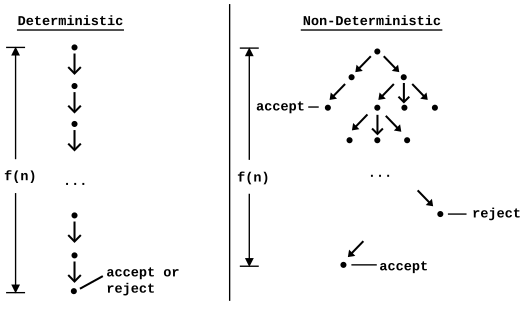
\includegraphics[width=0.6\linewidth]{Difference_between_deterministic_and_Nondeterministic.svg.png}
\end{center}
\begin{definition}[Time Complexity - Deterministica]
	La complessità temporale di una MdT \textit{decider\footnote{che termina per ogni input}} deterministica $M$ è una funzione $tc_M:\mathbb{N}\rightarrow\mathbb{N}$ dove
	\begin{center}
		\footnotesize
		$tc_M(n)$ = massimo numero di passi (transizioni) che $M$ esegue su qualunque input di lunghezza $n$
	\end{center}
\end{definition}
\begin{definition}[Time Complexity - Non deterministica]
	La complessità temporale di una MdT \textit{decider} non deterministica $M$ è una funzione $tc_M:\mathbb{N}\rightarrow\mathbb{N}$ dove
	\begin{center}
		\footnotesize
		$tc_M(n)$ = massimo numero di passi (transizioni) che $M$ esegue sul ramo più lungo, su qualunque input di lunghezza $n$
	\end{center}
\end{definition}
\begin{esempio}
	\footnotesize
	Se, per esempio, $tc_M(n)=6n^3+2n^2+3$ allora posso dire che:
	\begin{center}
		$tc_M(n)=O(n^3)$ dove $n$ è la lunghezza dell'input
	\end{center}
\end{esempio}


\subsection{$\mathcal{P}$}
La classe $\mathcal{P}$ è l'insieme dei linguaggi \textit{decisi}\footnote{un linguaggio L è decidibile se $\exists$ una MdT che decide $L$.} da una MdT (decider) \textcolor{red}{deterministica} in tempo polinomiale.
Quindi, è l'insieme dei linguaggi decidibili in tempo polinomiale. \\ \\
\textcolor{red}{Come dimostro che un algoritmo appartiene alla classe $\mathcal{P}$ ?}
\begin{enumerate}
	\item Descrivo l'algoritmo ad alto livello dividendolo in passi (ignorando i dettagli di nastri e testine).
	\item Mostro che il numero totale di passi dell'algoritmo, su input di lunghezza $n$, cresce al massimo come un polinomio. Uso notazione $O$-grande.
	\item Verifico che ciascun passo possa essere eseguito in tempo polinomiale su una MdT deterministica.
	\item Mi assicuro che la MdT costruita sia un decider, quindi che si arresti e fornisca una risposta per ogni input.
\end{enumerate}
\textcolor{red}{Codifica dei grafi:} Sia $G=(V,E)$ un grafo.
\begin{itemize}
	\item \textbf{Lista di adiacenza} (da usare quando il grafo è sparso\footnote{ha pochi archi rispetto ai nodi}): lista dove per ogni nodo del grafo vengono elencati altri nodi a cui è connesso.
	\item \textbf{Matrice di adiacenza} (da usare quando il grafo è denso\footnote{ha molti archi, quasi tutti i nodi collegati tra loro}): matrice quadrata dove l'elemento $(i,j)$ vale $1$
	      se esiste un arco dal nodo $i$ al nodo $j$, $0$ altrimenti.
\end{itemize}
\begin{osservazioni}[Osservazione]
	\footnotesize
	Quando analizziamo algoritmi su grafi, possiamo esprimere il tempo di esecuzione in base al numero di nodi del grafo, invece che della dimensione della rappresentazione del
	grafo (cioè della lunghezza dell’input codificato). Esempio: in un problema su grafi, l'algoritmo impiega tempo O($n^2$) dove $n$ è il numero di nodi del grafo.
\end{osservazioni}
\begin{esempio}[Esempio: codifica binaria della lista di adiacenza per MdT]
	\footnotesize
	Sia $G$ un grafo orientato $G=(V,E)$:
	\begin{itemize}
		\item $V = \{1, 2, 3\}$
		\item $E = \{(1,2), (1,3), (2,3)\}$
	\end{itemize}
	con la rappresentazione delle liste di adiacenza per ogni nodo: \\
	\begin{tabular}{c | l}
		\textbf{Nodo} & \textbf{Liste di adiacenza} \\ \hline
		1             & 2, 3                        \\
		2             & 3                           \\
		3             & -
	\end{tabular}
	\begin{center}
		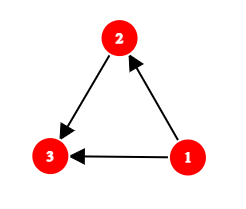
\includegraphics[width=0.3\linewidth]{graph1.png}
	\end{center}
	\textcolor{red}{Conversione in codifica binaria:}
	\begin{itemize}
		\item Sia $\Sigma = \{0, 1, \#\}$ l'alfabeto
		\item Il simbolo \textcolor{green}{$\#$} separa i nodi nella rispettiva lista di adiacenza
		\item Il simbolo \textcolor{red}{$\#\#$} separa le liste di adiacenza dei diversi nodi
		\item Il simbolo $\#\#\#$ indica la fine della lista
	\end{itemize}
	Pertanto: \\
	Nodo $1$: archi verso 2 e 3, quindi la codifica è 1\textcolor{green}{\#}10\textcolor{green}{$\#$}11\\
	Nodo $2$: arco verso 3, quindi la codifica è 10\textcolor{green}{$\#$}11\\
	Nodo 3: - \\
	Quindi l'intera codifica del grafo sarà 1\textcolor{green}{\#}10\textcolor{green}{$\#$}11\textcolor{red}{$\#\#$}10\textcolor{green}{$\#$}11\#\#\#
\end{esempio}
\begin{esempio}[Esempio: codifica binaria della matrice di adiacenza per MdT]
	\footnotesize
	Sia $G$ un grafo orientato $G=(V,E)$:
	\begin{itemize}
		\item $V = \{1, 2, 3\}$
		\item $E = \{(1,2), (1,3), (2,3)\}$
	\end{itemize}
	con la matrice di adiacenza associata:
	\begin{itemize}
		\item $i$ sono le righe
		\item $j$ sono le colonne
	\end{itemize}
	\[
		A[i,j] =
		\begin{array}{c|ccc}
			  & 1 & 2 & 3 \\ \hline
			1 & 0 & 1 & 1 \\
			2 & 0 & 0 & 1 \\
			3 & 0 & 0 & 0 \\
		\end{array}
	\]
	\textcolor{red}{Conversione in codifica binaria:}
	\begin{itemize}
		\item Sia $\Sigma = \{0, 1, \#\}$ l'alfabeto
		\item 0/1 valori nella matrice (assenza/presenza di arco)
		\item Il simbolo \textcolor{red}{$\#$} separa le righe
		\item Il simbolo $\#\#\#$ indica della codifica
	\end{itemize}
	Scrivo ogni riga (sequenza di bit) separata dal simbolo "\#", pertanto: \\
	Riga 1, per $i=1$: scrivo 011 \footnote{leggendo l'intera riga 1 vediamo la sequenza di bit 011} \\
	Riga 2, per $i=2$: scrivo 001 \\
	Riga 3, per $i=3$: scrivo 010 \\
	Quindi l'intera codifica della matrice di adiacenza è 011\textcolor{red}{\#}001\textcolor{red}{\#}000$\#\#\#$
\end{esempio}
\begin{center}
	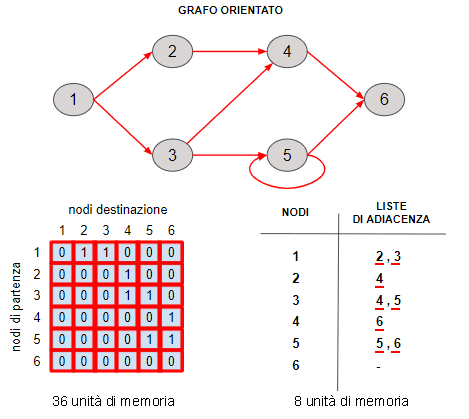
\includegraphics[width=0.7\linewidth]{lista-matrice-adiacenza-grafi.png}
\end{center}
\subsubsection{$PATH$}
Sia un grafo orientato $G$ che contiene i nodi $s$ e $t$. Il problema $PATH$ consiste nel determinare se esiste un cammino da $s$ a $t$.
\begin{center}
	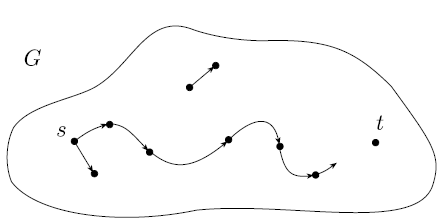
\includegraphics[width=0.4\linewidth]{path-problem.png}
\end{center}
\begin{theorem}{$PATH$ Problem}
	d$PATH = \{\langle G, s, t \rangle \mid G \text{ è un grafo orientato con cammino da } s \text{ a } t\}$
	\begin{center}
		$PATH \in \mathcal{P}$
	\end{center}
	\footnotesize
	\begin{ragionamento}
		Costruisco un algoritmo di decisione deterministico in tempo polinomiale per $PATH$. Uso l'algoritmo di ricerca in ampiezza\footnote{algoritmo BFS:
			\begin{enumerate}
				\item parto dal nodo sorgente $s$, lo aggiungo alla queue e lo segno come visitato
				\item finché la queue non è vuota:
				      \begin{enumerate}
					      \item estraggo un nodo $u$ dalla queue
					      \item per ogni nodo adiacente a $u$ non ancora visitato, aggiungilo alla queue e segnalo come visitato
				      \end{enumerate}
			\end{enumerate}
			L'algoritmo termina quando tutti i nodi raggiungibili da $s$ sono stati visitati. Se $t$ è tra i nodi visitati, allora esiste un cammino da $s$ a $t$.
		}.
	\end{ragionamento}
	\begin{proof}
		Costruisco una MdT $M$ deterministica a 2 nastri che decide $PATH$ come segue. Sia $\langle G, s, t\rangle$ la codifica del grafo orientato $G$ e dei nodi $s, t$.\\
		\textcolor{red}{1. Costruzione della MdT $M$} \\
		$M$ su input $\langle G, s, t \rangle$:
		\begin{enumerate}
			\item Marca il nodo $s$ come visitato sul secondo nastro
			\item Ripeti quanto segue finchè si possono marcare nuovi nodi\footnote{\underline{Attenzione:} non scrivo "finché tutti i nodi non vengono visitati" perchè
				      se alcuni nodi non sono raggiungibili da $s$, non verranno mai marcati — quindi il ciclo “finché tutti” non terminerebbe mai.}:
			      \begin{enumerate}
				      \item Scorri tutti gli archi del grafo $G$ sul nastro 1.
				      \item Se trovi un arco $(u,v)$ che va da un nodo $u$ già visitato a un nodo $v$ non visitato, allora marca $v$ sul nastro 2.
			      \end{enumerate}
			\item Se $t$ è marcato come visitato\footnote{esite un cammino da $s$ a $t$}, allora accetta. Altrimenti, rifiuta.
		\end{enumerate}
		\textcolor{red}{2. Analisi della complessità temporale della MdT $M$}
		\begin{enumerate}
			\item Verifico che ciascun passo possa essere eseguito in tempo polinomiale su una MdT deterministica:
			      \begin{itemize}
				      \item \textbf{Passo 1:} operazione che, indipendentemente dalla dimensione del grafo, ha sempre tempo costante O$(1)$.
				      \item \textbf{Passo 2:} questo passo (ciclo, ripetuto massimo $n$ volte dove $n$ sono i nodi) fa il lavoro grosso:
				            \begin{itemize}
					            \item Scorre tutti gli archi $e$ del grafo, tempo O$(e)$
					            \item Controlla se, per ogni arco $(u,v)$, $u$ è stato visitato e $v$ no (ricerca nel nastro 2, tempo O($n$))
					            \item Se trovo un arco valido, allora marco $v$ come visitato (marcatura tempo O(1))
				            \end{itemize}
				            Pertanto, ho O($n)\cdot \big[O(e)\cdot O(n)\cdot O(1)\big]=O(n)\cdot \big[O(e \cdot n)\big]=O(e \cdot n^2)$
				      \item \textbf{Passo 3:} operazione che, indipendentemente dalla dimensione del grafo, ha sempre tempo costante O$(1)$.
			      \end{itemize}
			\item Mostro che il numero tot di passi dell'algoritmo, su input di lunghezza $n$, cresce al massimo come un polinomio:
			      \begin{itemize}
				      \item \textbf{Passo 1:} tempo O(1)
				      \item \textbf{Passo 2:} tempo O($e \cdot n^2$)
				      \item \textbf{Passo 3:} tempo O(1)
			      \end{itemize}
			      Pertanto, la complessità nel caso pessimo dell'algoritmo è:
			      \begin{center}
				      $tC_M(x)$=O(1)+O($e \cdot n^2$)+O(1)=\textcolor{red}{O($e \cdot n^2$)} \\ dove "$n$" sono i nodi, "$e$" gli archi e "$x$" è la lunghezza dell'input $\langle G, s, t \rangle$
			      \end{center}
			      La complessità è quindi polinomiale. \\
		\end{enumerate}
		\underline{Conclusione:} Ho costruito una MdT $M$ deterministica che decide $PATH$ in tempo polinomiale. Quindi, $PATH \in \mathcal{P}$.
	\end{proof}
\end{theorem}

\subsubsection{$RELPRIME$}
Due numeri $x$ e $y$ sono relativamente primi se 1 è l'unico numero intero che li divide entrambi. Per esempio, 4 e 8 non sono relativamente primi perchè 2 li divide entrambi.
\begin{theorem}{RELPRIME Problem}
	d$RELPRIME = \{\langle x,y \rangle \mid x \text{ e } y \text{ sono relativamente primi}\}$
	\begin{center}
		$RELPRIME \in \mathcal{P}$
	\end{center}
	\footnotesize
	\begin{ragionamento}
		Costruisco un algoritmo di decisione determinisitco in tempo polinomiale per $RELPRIME$. Uso l'algoritmo di Euclide per calcolare il $mcd$.
		\begin{center}
			$x$ e $y$ sono relativamente primi $\iff mcd(x,y)=1$
		\end{center}
	\end{ragionamento}
	\begin{proof}
		\textcolor{red}{1. Algoritmo di Euclide:} \\
		Sia $E$ la MdT che calcola il massimo comune divisore di $x$ e $y$ usando l'algoritmo di Euclide. \\ \\
		$E$ su input $\langle x,y \rangle$ dove $x$ e $y$ sono numeri naturali in codifica binaria:
		\begin{enumerate}
			\item Ripeti finchè $y \neq 0$:
			      \begin{enumerate}
				      \item Calcola $x$ mod $y$ e assegna il valore a $x$ ($x \leftarrow x$ mod $y$)
				      \item Scambia $x$ e $y$ ($swap(x,y)$)
			      \end{enumerate}
			\item Restituisci $x$ (l'output che alla fine sarà il $mcd$)
		\end{enumerate}
		\textcolor{red}{2. Costruisco MdT che decide $RELPRIME$:} \\
		Costruisco la MdT $R$ che simula la MdT $E$. \\ \\
		$R$ su input $\langle x,y \rangle$ dove $x$ e $y$ sono numeri naturali in codifica binaria:
		\begin{enumerate}
			\item Esegue $E$ su $\langle x,y \rangle$:
			      \begin{itemize}
				      \item Se $E$ restituisce 1, allora $R$ accetta.
				      \item Se $E$ restituisce un altro valore diverso da 1, allora $R$ rifiuta.
			      \end{itemize}
		\end{enumerate}
		Quindi $R$ accetta solo se $mcd(x,y)=1$, rifiuta altrimenti. Pertanto $R$ è una MdT che decide correttamente $RELPRIME$. Adesso analizzo la complessità. \\
		\textcolor{red}{3. Analisi della complessità temporale}
		\begin{enumerate}
			\item Analizzo ciascun passo della MdT $E$:
			      \begin{itemize}
				      \item \textbf{Passo 1.a:} il calcolo del modulo richiede tempo O($n^2$), l'assegnazione $x=x$ mod $y$ richiede tempo O($n$); quindi O($n^2$)+O($n$)=O($n^2$)
				      \item \textbf{Passo 1.b:} scambiare $x$ e $y$ richiede tempo O($n$)
				      \item \textbf{Passo 1:} Quante iterazioni servono affinchè $y=0$? O($\log_2x$)=O($n$)
				      \item \textbf{Passo 2:} restituire il valore di $x$ richiede tempo O($n$)
			      \end{itemize}
			      Nel passo 1: $O(\log_2x)\cdot\big[O(n^2)+O(n)\big]=O(\log_2x)\cdot\big[O(n^2)\big]=O(n)\cdot\big[O(n^2)\big]=\textcolor{red}{O(n^3)}$ \\
			      Nel passo 2: $O(n)$
			\item Mostro che il numero tot di passi dell'algoritmo, su input di lunghezza n, cresce
			      al massimo come un polinomio:
			      \begin{itemize}
				      \item La MdT $E$: O($n^3$)
				      \item La MdT $R$ che simula $E$ ha O($n^3$) e poi accetta o rifiuta in base a cosa restituisce $E$, quindi O($n$)
			      \end{itemize}
			      Pertanto, la complessità è $tC_R(n)=O(n^3)+O(n)=O(n^3)$ dove $n$ è la lunghezza dell'input, quindi polinomiale.
		\end{enumerate}
		\underline{Conclusione:} Ho costruito una MdT $R$ determinisitca che decide $RELPRIME$ in tempo polinomiale. Quindi, $RELPRIME \in \mathcal{P}$
	\end{proof}
\end{theorem}
\subsubsection{$2-SAT$}
%%%%%%%%%%%%%%%%%%%%%%%%%%%%%%%%%%%%%%%%%%%%%%%%%%%%%%%%%%%%%%%%%%%%%%%%%%%%%%%%%%%%%%%%%%%%%%%%%%%%%%
%%%%%%%%%%%%%%%%%%%%%%%%%%%%%%%%%%%%%%%%%%%%%%%%%%%%%%%%%%%%%%%%%%%%%%%%%%%%%%%%%%%%%%%%%%%%%%%%%%%%%%
\subsection{$\mathcal{NP}$}
La classe $\mathcal{NP}$ è l'insieme dei linguaggi \textit{decisi}\footnote{un linguaggio
	L è decidibile se $\exists$ una MdT che decide $L$.} da una MdT (decider) \textcolor{red}{non deterministica} in tempo polinomiale.
Quindi, è l'insieme dei linguaggi decidibili in tempo polinomiale.
\begin{osservazioni}[Osservazione]
	\footnotesize
	La classe $\mathcal{NP}$ è l'insieme dei linguaggi:
	\begin{itemize}
		\item risolvibili da una MdT non deterministica in tempo polinomiale (senza certificato), oppure
		\item verificabili da una MdT deterministica in tempo polinomiale, dato come input un certificato
	\end{itemize}
\end{osservazioni}
\begin{table}[h!]
	\centering
	\footnotesize
	\begin{tabular}{|l|c|c|}
		\hline
		\rowcolor{gray!30}
		\textbf{Tipo di MdT}                                & \textbf{Input}        & \textbf{Richiede certificato?} \\
		\hline
		\cellcolor{blue!15} Non Deterministica              & istanza               & No                             \\
		\hline
		\cellcolor{yellow!15} Deterministica (verificatore) & istanza + certificato & Sì                             \\
		\hline
	\end{tabular}
	\caption{Differenza tra MdT nondeterministica e MdT deterministica (verificatore) nei problemi NP}
\end{table}

\subsubsection{Riduzione polinomiale}
Ricorda la notazione $f$: input $\rightarrow$ output
\begin{definition}[Funzione di riduzione in tempo polinomiale]
	Sia $L_1$,$L_2$ due linguaggi su $\Sigma_{1}^*,\Sigma_{2}^*,$ rispettivamente.
	Si dice che $L_1$ è polinomialmente riducibile a $L_2$, e si scrive \textcolor{red}{$L_1 \leq_{p} L_2$} se $\exists$ una funzione computabile totale calcolabile in tempo polinomiale
	$f:\Sigma^*_1 \rightarrow \Sigma^*_2$ chiamata \textbf{funzione di riduzione in tempo polinomiale} t.c. $\forall{w}\in \Sigma^*_1$
	\begin{align*}
		w \in L_1 \iff f(w) \in L_2
	\end{align*}
	Spiegazione informale:\\
	Per effetturare una riduzione da $L_1$ a $L_2$, deve esistere una MdT $R$ (macchina di riduzione) che prende in input
	una qualunque stringa $w \in \Sigma^*_1$ e la trasforma in una stringa $f(w) \in \Sigma^*_2$.
	Ovvero, se la MdT $R$ prende in input un'istanza di $L_1$ allora produce come output un'istanza di $L_2$. \\
	La MdT $R$ calcola la funzione di riduzione $f$ in tempo polinomiale. \\
	In questo modo, se avessimo una MdT che decide $L_2$, potremmo decidere $L_1$ applicando $f$.
\end{definition}
\begin{theorem}{5.2.1.1}
	SSe $L_1 \leq_p \textcolor{red}{L_2}$ e $\textcolor{red}{L_2 \in \mathcal{P}}$, allora $L_1 \in \mathcal{P}$
\end{theorem}
\begin{theorem}{5.2.1.2}
	SSe $L_1 \leq_p \textcolor{red}{L_2}$ e $\textcolor{red}{L_2 \in \mathcal{NP}}$, allora $L_1 \in \mathcal{NP}$
\end{theorem}

\subsubsection{$\mathcal{NP}$-Hard}
Un problema $L$ è $\mathcal{NP}$-Hard (o $\mathcal{NP}$-Difficile) se tutti i problemi in $\mathcal{NP}$ si possono ridurre a $L$ in tempo polinomiale.
\begin{theorem}{$\mathcal{NP}$-Hard}
	sUn linguaggio $\textcolor{red}{L}$ è $\mathcal{NP}$-Hard se: \\ $\forall{Q}$ linguaggio $\in \mathcal{NP}$, $\exists f$ riduzione
	polinomiale da $Q$ a $L$ ($Q \leq_p \textcolor{red}{L}$).
\end{theorem}
\begin{theorem}{$\mathcal{NP}$-Hard}
	sSe $L_1 \leq_p \textcolor{red}{L_2}$ e \textcolor{red}{$L_1$ è $\mathcal{NP}$-Hard}, allora $L_2$ è $\mathcal{NP}$-Hard
\end{theorem}
Un problema $L$ può:
\begin{itemize}
	\item essere $\mathcal{NP}$-Hard $\land \in \mathcal{NP}$, oppure
	\item essere $\mathcal{NP}$-Hard $\land \notin \mathcal{NP}$
\end{itemize}
Se $B$ è $\mathcal{NP}$-Hard $\land$ $B \in \mathcal{NP} \implies B$ è $\mathcal{NP}$-Completo.
\subsubsection{$\mathcal{NP}$-Completo}
\begin{theorem}{$\mathcal{NP}$-Completo}
	sUn linguaggio $L$ è $\mathcal{NP}$-Completo se:
	\begin{itemize}
		\item $L \in \mathcal{NP}$, e
		\item $L \in \mathcal{NP}$-Hard
	\end{itemize}
\end{theorem}
\begin{theorem}{5.2.3}
	s
	\begin{itemize}
		\item $B$ è $\mathcal{NP}$-Completo
		\item $C \in \mathcal{NP}$
	\end{itemize}
	Se $B \leq_p C$, allora $C$ è $\mathcal{NP}$-Completo.
\end{theorem}


%%%%%%%%%%%%%%%%%%%%%%%%%%%%%%%%%%%%%%%%%%%%%%%%%%%%%%%%%%%%%%%%%%%%%%%%%%%%%%%%%%%%%%%%%%%%%%%%%%%%%%
%%%%%%%%%%%%%%%%%%%%%%%%%%%%%%%%%%%%%%%%%%%%%%%%%%%%%%%%%%%%%%%%%%%%%%%%%%%%%%%%%%%%%%%%%%%%%%%%%%%%%%
\subsubsection{Polinomio Booleano}
\begin{definition}[Variabile booleana] Una \textcolor{red}{variabile booleana} è una variabile $x$ che assume solo due valori:
	\begin{itemize}
		\item $x=0$ (falso)
		\item $x=1$ (vero)
	\end{itemize}
\end{definition}
\textcolor{red}{Operatori logici:}
\begin{itemize}
	\item AND, indicato con il simbolo $\land$
	\item OR, indicato con il simbolo $\lor$
	\item NOT, indicato con il simbolo $\lnot$
\end{itemize}
\begin{center}
	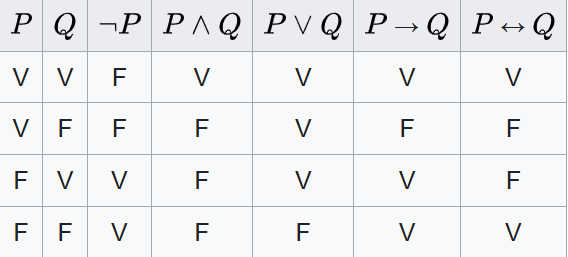
\includegraphics[width=0.6\linewidth]{boolean-exp.png}
\end{center}
\begin{definition}[Letterale]
	Un \textcolor{red}{letterale} $x$ è una variabile booleana o la sua negazione $\overline{x}$.
\end{definition}
\begin{definition}[Clausola]
	Una \textcolor{red}{clausola} è una disgiunzione di letterali:
	\[
		(x_1 \lor \cdots \lor x_n)
	\]
	La clausola è vera se almeno uno dei suoi letterali è vero.
\end{definition}
\begin{definition}[CNF]
	Una formula è in \textcolor{red}{forma normale congiuntiva} se è una congiunzione ($\land$) di clausole (dove le clausole sono una disgiunzione di letterali):
	\[
		\underbrace{(x_{1,1} \lor \dots \lor x_{1,n})}_{\text{clausola 1}}
		\land
		\underbrace{(x_{2,1} \lor \dots \lor x_{2,n})}_{\text{clausola 2}}
		\land \dots \land
		\underbrace{(x_{n,1} \lor \dots \lor x_{n,n})}_{\text{clausola n}}
	\]
	La formula in CNF è vera se tutte le clausole sono vere.
\end{definition}
\begin{definition}[Formula booleana]
	Un \textcolor{red}{formula booleana} è un'espressione costruita con:
	\begin{itemize}
		\item letterali (positivi o negativi)
		\item operatori logici ($\land, \lor, \lnot$)
	\end{itemize}
\end{definition}
\begin{definition}[Polinomio booleano]
	Un \textcolor{red}{polinomio booleano} è un'espressione costruita con:
	\begin{itemize}
		\item letterali (positivi o negativi)
		\item operatori aritmetici in cui:
		      \begin{itemize}
			      \item ($\lnot x$) corrisponde a $1-x$
			      \item ($x \land y$) corrisponde a $x \cdot y$
			      \item ($x \lor y$) corrisponde a $x + y - x \cdot y$
		      \end{itemize}
	\end{itemize}
	Quindi il polinomio booleano è la rappresentazione algebrica della formula booleana.
\end{definition}
\begin{esercizio}[Esempio]
	\footnotesize
	Date le variabili $\{x_1,x_2,x_3\}$, una formula booleana in CNF può essere:
	\[
		f = (x_1 \lor \overline{x_2}) \land (\overline{x_1} \lor x_3)
	\]
	mentre il corrispondente polinomio booleano è:
	\begin{center}
		$p = (x_1 \lor (1-x_2)) \land ((1-x_1) \lor x_3)$ \\
		$= \big[(x_1+(1-x_2))-(x_1 \cdot (1-x_2))\big] \land \big[((1-x_1)+x_3) - ((1-x_1)\cdot x_3)\big]$ \\
		$= \big[(x_1+(1-x_2))-(x_1 \cdot (1-x_2))\big] \cdot \big[((1-x_1)+x_3) - ((1-x_1)\cdot x_3)\big]$ \\
		sviluppando e sapendo che per proprietà booleana $x_i^2=x_i$ allora ottengo: \\
		$= x_1x_2+x_1x_3-x_1-x_2+1$
	\end{center}

\end{esercizio}
%%%%%%%%%%%%%%%%%%%%%%%%%%%%%%%%%%%%%%%%%%%%%%%%%%%%%%%%%%%%%%%%%%%%%%%%%%%%%%%%%%%%%%%%%%%%%%%%%%%%%%
%%%%%%%%%%%%%%%%%%%%%%%%%%%%%%%%%%%%%%%%%%%%%%%%%%%%%%%%%%%%%%%%%%%%%%%%%%%%%%%%%%%%%%%%%%%%%%%%%%%%%%
\subsubsection{$SAT$}
Data una formula booleana $f$ scritta in CNF, esiste un qualche assegnamento di valori (0/1) alle variabili che rende l'intera formula $f$ vera\footnote{la formula booleana
	restituisce come output 1}?
\begin{osservazioni}[Osservazione]
	\footnotesize
	Il numero di letterali in ogni clausola può variare; non c'è un limite fisso. \\
	Per esempio:
	\begin{center}
		$(x \lor y) \land (\overline{z} \lor w \lor u) \land (v)$
	\end{center}
	Nella prima clausola ci sono 2 lettarli, nella seconda 3 e nell'ultima 1.
\end{osservazioni}
\begin{theorem}{$SAT$ Problem}
	gData $f$, una formula booleana in CNF, determinare se $\exists$ un qualche assegnamento di valori alle variabili che renda $f$ vera.
	\begin{center}
		$SAT = \{\langle f \rangle \mid f \text{ è una cnf-formula booleana soddisfacibile}\}$ \\
		$SAT \in \mathcal{NP}$
	\end{center}
	\footnotesize
	\begin{proof}
		Sia $\{x_1,x_2,...,x_n\}$ l'insieme delle variabili booleane. \\
		\textbf{\textcolor{red}{1. Codifica}} \\
		Ogni variabile è codificata in binario come segue: numero del letterale in binario seguito da $\#1$ se il letterale è positivo
		oppure $\#0$ se il letterale è negativo. \\ \\
		\begin{tabular}{|c|c|}
			\hline
			\textbf{Letterale} & \textbf{Codifica} \\ \hline
			$x_i$              & $i \# 1$          \\ \hline
			$\lnot x_i$        & $i \# 0$          \\ \hline
		\end{tabular} \\ \\
		Esempio: \\
		Sia $f$ in CNF: $(x_1 \lor \overline{x_2}) \land (\overline{x_1} \lor x_3)$. Verrà codificato come:
		\[
			1\#1 \lor 10\#0 \land 1\#0 \lor 11\#1
		\]
		\\
		La codifica finale in input alla MdT sarà composta da:
		\begin{itemize}
			\item una lista di interi da 1 a $n$ in binario separati dal simbolo \# (che indicano le variabili presenti nella formula)
			\item codifica della formula booleana
		\end{itemize}
		la lista e la formula sono separati dal simbolo \#\#. \\ \\
		Esempio: \\
		Sia $f$ in CNF: $(x_1 \lor \overline{x_2}) \land (\overline{x_1} \lor x_3)$. La codifica in input alla MdT sarà:
		\[
			\underbrace{1\#10\#11}_{\text{variabili}}
			\#\#
			\underbrace{1\#1 \lor 10\#0 \land 1\#0 \lor 11\#1}_{\text{formula booleana}}
		\]
		\textbf{\textcolor{red}{2. Alfabeto e Linguaggio}}
		\begin{itemize}
			\item Sia $\Sigma_{SAT} = \{0,1,\#,\land,\lor\}$ l'alfabeto del problema $SAT$.
			\item Sia $L_{SAT}$ oppure semplicemente $SAT$ il linguaggio del problema, ovvero l'insieme di tutte le formule booleane per cui esiste un assegnamento che le rende vere. \\
			      $L_{SAT} = \{\langle f \rangle \mid f \text{ formula booleana soddisfacibile}\}$
		\end{itemize}
		\textbf{\textcolor{red}{3. Costruzione della MdT non deterministica}} \\
		Costruisco una MdT $S$ non deterministica che decide $SAT$ in tempo polinomiale. \\
		$S$ ha due nastri:
		\begin{itemize}
			\item \textbf{Nastro 1:} codifica finale
			\item \textbf{Nastro 2:} nastro di lavoro che genera su di esso (non deterministicamente) un assegnamento alle variabili come segue:
			      \[
				      x_1\#t(x_1)\textcolor{red}{\#\#}x_2\#t(x_2)\textcolor{red}{\#\#}\cdots x_n\#t(x_n)
			      \]
			      dove:
			      \begin{itemize}
				      \item $x_i$ è la rappresentazione binaria dell'indice $i$ della variabile corrispondente
				      \item $t(x_i)$ indica l'assegnamento del valore alla variabile $x_i$, che può essere 1 o 0
			      \end{itemize}
		\end{itemize}
		Esempio grafico dei nastri nel caso della formula $(x_1 \lor \overline{x_2}) \land (\overline{x_1} \lor x_3)$:
		\begin{center}
			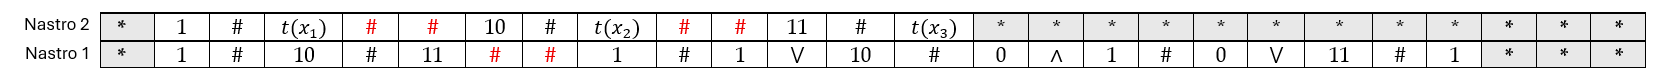
\includegraphics[width=1.04\linewidth]{sat-tapes-mdt.png}
		\end{center}
		\textbf{\textcolor{red}{4. Funzionamento della MdT $S$ non deterministica}} \\
		$S$ è la MdT non deterministica e $\langle f \rangle$ è codifica finale sopra descritta. \\ \\
		$S$ su input $\langle f \rangle$: \\
		Sul nastro 1 ho la codifica finale di $f$ e il nastro 2 è vuoto.
		\begin{enumerate}
			\item $S$ controlla che la stringa in input sul nastro 1 sia sintatticamente corretta; se non lo è, rifiuta.
			\item $S$ sul nastro 2 genera (non deterministicamente) un assegnamento alle variabili.
			\item $S$ esamina l'input sul nastro 1 da sinistra verso destra, fino ad incontrare un letterale:
			      \begin{enumerate}
				      \item Confronta il letterale della clausola sul nastro 1 $v\#t(v)$ con l'assegnamento corrispondente sul nastro 2 $x_i\#t(x_i)$:
				            \begin{itemize}
					            \item Se corrispondono, la clausola è soddisfatta (basta un assegnamento vero per rendere vera l'intera clausola vera);
					                  \begin{itemize}
						                  \item Se la clausola appena esaminata era l'ultima, allora $S$ accetta e termina ($f \in SAT$).
						                  \item Se la clausola appena esaminata non era l'ultima, allora passo alla clausola successiva;
					                  \end{itemize}
					            \item Se non corrispondono, esamino il letterale successivo;
					                  \begin{itemize}
						                  \item Se il letterale appena esaminato è l'ultimo della clausola, allora $S$ rifiuta e termina ($f \notin SAT$).
						                  \item Se il letterale appena esaminato non è l'ultimo della clausola, allora passa al letterale successivo;
					                  \end{itemize}
				            \end{itemize}
			      \end{enumerate}

			      \textbf{Spiegazione dettagliata:} \\
			      A seguito viene spiegato il comportamento di $S$ con ciclo interno ed esterno perchè cosi è più facile calcolare la complessità.
			      \textcolor{red}{Ricordo che la formula è vera se tutte le sue clausole sono vere (dove ogni clausola è vera se almeno uno dei valori è vero)}.
			      \begin{enumerate}
				      \item Ciclo esterno: scansiona tutte le clausole della formula
				      \item Ciclo interno: scansione ogni letterale della clausola
			      \end{enumerate}

			      \begin{itemize}
				      \item Per ogni clausola della formula booleana (ciclo esterno):

				            \begin{itemize}
					            \item Per ogni letterale della clausola (ciclo interno):
					                  \begin{enumerate}
						                  \item Confronta il letterale sul nastro 1 $v\#t(v)$ con l'assegnamento corrispondente sul nastro 2 $x_1\#t(x_1)$:
						                        \begin{itemize}
							                        \item Se coincidono, la clausola è soddisfatta, quindi esci dal ciclo interno (uscendo dal ciclo interno va allo step (a) sotto)
							                        \item Se non coincidono e il letterale esaminato è l'ultimo della clausola, $S$ rifiuta e termina; Altrimenti passa al prossimo letterale.
						                        \end{itemize}
					                  \end{enumerate}
				            \end{itemize}
				            \begin{enumerate}
					            \item Se la clausola è l'ultima dell'intera formula booleana, allora $S$ accetta e termina.\footnote{non importa specificare che la clausola è soddisfatta perchè questo passo
						                  della computazione è eseguibile uscendo dal ciclo interno solo quando la clausola è soddisfatta}
					            \item Se la clausola non è l'ultima dell'intera formula booleana, allora passa alla prossima clausola.
				            \end{enumerate}
			      \end{itemize}


		\end{enumerate}
		\textbf{\textcolor{red}{5. Complessità della MdT $S$}}
		\begin{enumerate}
			\item Analizzo complessità ciclo interno: (ripetuto per $n$ letterali in caso pessimo) \\
			      In questo caso il caso pessimo è quando analizza tutti i letterali fino all'ultimo della clausola.
			      Confronto costa $O(\log_2n)$ sul nastro 1 e $O(\log_2n)$ sul nastro 2 perchè deve leggere e muovere la testina in base a quanto è lungo il letterale in esame (in codifica binaria). \\
			      Approssimativamente, ripeto il ciclo per $n$ letterali, quindi la complessità è $n \cdot O(\log_2n) = O(n \log_2n)$.
			\item Analizzo complessità ciclo esterno: (ripetuto per $n$ clausole della formula booleana in caso pessimo) \\
			      In questo caso il caso pessimo è quando analizza tutte le clausole dell'intera formula.
			      Approssimativamente, costa $O(n)$.
		\end{enumerate}
		Mettendo tutto insieme, la complessità di $S$ è $O(n \log_2n) \cdot O(n)=O(n^2 \log_2n)$ e quindi polinomiale. \\ \\
		\underline{Conclusione:} La MdT $S$ non deterministica decide $SAT$ in tempo polinomiale. Pertanto, $SAT \in \mathcal{NP}$
	\end{proof}
\end{theorem}

\begin{theorem}{Teorema di Cook-Levin}
	d$SAT$ è $\mathcal{NP}$-Hard.
	\footnotesize
	\begin{ragionamento}
		Devo costruire una funzione di riduzione in tempo polinomiale in modo che ogni problema in $\mathcal{NP}$ possa essere riducibile a $SAT$. Ma i problemi in $\mathcal{NP}$
		sono infiniti, non posso provarli tutti, non finirei mai. Dato che ogni problema $\mathcal{NP}$ è per definizione decidibile da una MdT non deterministica in tempo polinomiale,
		per fare la riduzione uso il concetto di \textit{tableau}. \\
		Il \textcolor{red}{tableau} è una rappresentazione generica dell'esecuzione di una macchina non deterministica, quindi il tableau \textcolor{red}{può simulare qualsiasi macchina
			non deterministica che lavora in tempo polinomiale}. In questo modo posso rappresentare qualsiasi problema $\mathcal{NP}$.
		\begin{center}
			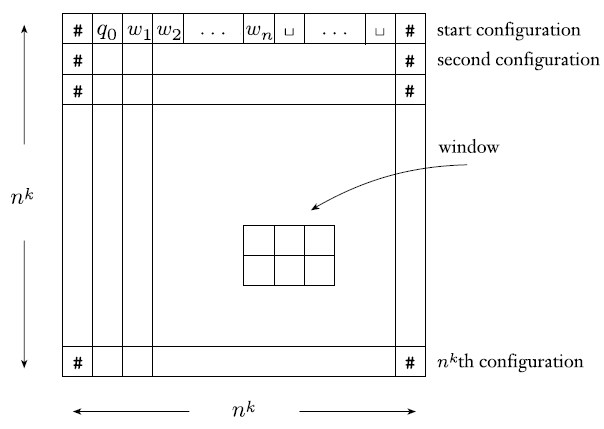
\includegraphics[width=0.8\linewidth]{tableau.png}
		\end{center}
		Osservazioni sul tableau: \\
		È una tabella $n^k \times n^k$ dove ogni riga rappresenta "la fotografia" della MdT in un instante di tempo. \\ Le righe rappresentano le configurazioni di un ramo della computazione
		di una MdT su un input $w$ (l'intero tableau rappresenta solo un ramo di computazione, non è che ogni riga rappresenta
		un ramo diverso).
		\begin{itemize}
			\item \textbf{Tableau:} tabella che mostra tutte le configurazioni di un singolo ramo.
			\item  \textbf{Riga del tableau:} Una configurazione (stato $q_i$ + contenuto nastro + posizione testina).
		\end{itemize}
	\end{ragionamento}
	\begin{proof}
		Sia $A$ un generale problema $\mathcal{NP}$ e sia $N$ la MdT non deterministica che decide $A$ in tempo polinomiale. \\
		\textcolor{red}{\textbf{1. Tableau per MdT non deterministica $N$}} \\
		Adesso descrivo il tableau per la MdT non deterministica $N$ su input $w$:
		\begin{itemize}
			\item \textbf{La prima riga:} configurazione iniziale di $N$. \\
			      (\textit{esempio: la macchina parte nello stato iniziale $q_0$ con l'input scritto sul nastro e la testina sulla prima cella dell'input})
			\item \textbf{La seconda riga:} rappresenta lo stato della macchina dopo il primo passo della computazione. \\
			      \vdots
			\item \textbf{La $i$-esima riga:} rappresenta lo stato della macchina dopo l' $i-1$-esimo passo della computazione.
		\end{itemize}
		Assumo che ogni riga (configurazione) abbia come simbolo \# nella prima e nell'ultima cella. \\
		Inoltre, un tableau è detto accettante se almeno una delle sue righe è una configurazione accettante; In altre parole, se troviamo un tableau accettante,
		sappiamo che esiste un ramo della MdT non deterministica che accetta l'input $w$.
		Per sapere se la macchina $N$ accetta $w$, basta verificare se esiste almeno un tableau accettante (perchè per ogni ramo esiste un tableau). \\
		\textcolor{red}{\textbf{2. Descrizione della funzione di riduzione $f$}} \\
		Sia $w$ un'istanza del problema $A$ e sia $f(w)$ un'istanza del problema $SAT$. Con input $w$, la funzione di riduzione produce come output la formula booleana $f(w)=\phi$. \\
		\begin{enumerate}
			\item \textcolor{blue}{\textbf{Descrivo le variabili booleane della formula $\phi$}} (delle parti di $\phi$?)
			      \begin{itemize}
				      \item Sia $Q$ l'insieme degli stati di $N$
				      \item Sia $\Gamma$ l'alfabeto del nastro di $N$
				      \item Sia $C= Q \cup \Gamma \cup \{\#\}$
				      \item Sia $s \in C$ un simbolo che può apparire in una cella del tableau \\ (ogni cella può contenere uno solo dei simboli in $C$:
				            o uno stato, o un simbolo del nastro, o il simbolo \#)
			      \end{itemize}
			      Per ogni cella $[i,j]$ e per ogni simbolo $s \in C$, ho la variabile booleana $x_{i,j,s}$ dove:
			      \[
				      x_{i,j,s} =
				      \begin{cases}
					      1 & \text{se la cella } [i,j] \text{ contiene il simbolo } s \\
					      0 & \text{altrimenti}
				      \end{cases}
			      \]
			      Esempio nelle note\footnote{$x_{0,2,q_1}=1$ la variabile vale 1 perchè la cella della riga 0 e della colonna 2 contiene il simbolo $q_1$.}
			\item \textcolor{blue}{\textbf{Descrivo la formula $\phi$}} \\
			      Costruisco la formula booleana $\phi$ tale che un'assegnazione di valori che soddisfa $\phi$ rappresenta un tableau accettante della macchina $N$ sull'input $w$, ovvero:
			      \begin{center}
				      $\phi$ è soddisfacibile $\iff N$ accetta $w$
			      \end{center}
			      La formula \textcolor{red}{$\phi$} è composta da 4 sottoformule, congiunte tra loro mediante l'operatore logico AND:
			      \[
				      \phi = \varphi_{cell} \land \varphi_{start} \land \varphi_{move} \land \varphi_{accept}
			      \]
			\item \textcolor{blue}{\textbf{Descrivo ogni sottoformula $\varphi$ di $\phi$}}
			      \begin{itemize}
				      \item $\varphi_{cell}$:  ogni cella contiene esattamente un simbolo (solo uno).
				      \item $\varphi_{start}$: la prima riga del tableau rappresenta lo stato iniziale di $N$ su $w$.
				      \item $\varphi_{move}$:  ogni riga del tableau segue la precedente secondo le regole di $N$
				            (assicura che ogni computazione segua legalmente la precedente secondo le regole di $N$)
				      \item $\varphi_{accept}$: almeno in una cella appare lo stato di accettazione $q_{accept}$.
			      \end{itemize}
		\end{enumerate}
		Ogni sottoformula diventa vera se è vera anche nel tableau.
		Quindi la formula $\phi = \varphi_{cell} \land \varphi_{start} \land \varphi_{move} \land \varphi_{accept}$ è vera
		se e solo se ogni $\varphi_i$ è vera. \\
		In poche parole, se il tableau è un tableau accettante ($N$ accetta $w$), allora $\phi$ è vera/soddisfacibile.

		\textcolor{red}{\textbf{3. Calcolo complessità della funzione di riduzione $f$}} \\
		Preso in input qualunque stringa $w$, voglio dimostrare che posso costruire un'istanza di $SAT$ in tempo polinomiale.
		Ovvero dato in input $w$, la funzione di riduzione $f$ restituisce $f(w)=\varphi_{cell} \land \varphi_{start} \land \varphi_{move} \land \varphi_{accept}$
		in tempo polinomiale rispetto alla lunghezza dell'input $w$. $f(w)=\phi$.
		\begin{enumerate}
			\item \textbf{Esamino la dimensione di $\phi$, ovvero quante variabili ha (le variabili sono le $x_{i,j,s}$):}
			      La tabella ha dimensione $n^k \times n^k$ e quindi ci sono $n^{2k}$ celle. Per ogni cella ci sono tante variabili quante sono le possibilità
			      di simbolo $s \in C$, quindi la complessità è $|C|\cdot O(n^{2k})$ e quindi \textcolor{red}{$O(n^{2k})$}.
			\item \textbf{Analizzo ogni parte della formula $\phi$:}
			      \begin{enumerate}
				      \item $\varphi_{cell}$: ogni cella contiene esattamente uno dei simboli di $C$, $O(n^{2k})$
				      \item $\varphi_{start}$: la prima riga è la configurazione iniziale di $N$ su $w$; ogni riga contiene $n^k$ celle, quindi $O(n^k)$
				      \item $\varphi_{move}$: ogni riga segue la precedente secondo le regole di $N$, $O(n^{2k})$
				      \item $\varphi_{accept}$: almeno una cella contiene lo stato di accettazione $q_{accept}$, controllo tutte le celle nel caso peggiore e quindi $O(n^{2k})$
			      \end{enumerate}
		\end{enumerate}
		Pertanto la complessità finale di $\phi$ è $O(n^{2k})+O(n^{k})+O(n^{2k})+O(n^{2k})=\textcolor{red}{O(n^{2k})}$ quindi polinomiale.\\
		Quindi la riduzione è polinomiale. \\

		\textcolor{red}{\textbf{4. La formula $\phi$ non è in CNF}} \\
		La formula booleana $f(w)$ ovvero $\phi = \varphi_{cell} \land \varphi_{start} \land \varphi_{move} \land \varphi_{accept}$ non è in CNF.
		Tuttavia, il problema $SAT$ richiede che l'input sia una formula in CNF. Come posso fare?
		Applico la \textcolor{red}{trasformazione di Tseitin}, che prende in input una formula booleana arbitraria e restituisce la formula in CNF
		equisoddisfacibile. Tutto ciò in tempo polinomiale.

		\[
			w \xrightarrow[\text{polinomiale}]{\text{Cook–Levin}} \phi
			\xrightarrow[\text{polinomiale}]{\text{Tseitin}} \phi_{\text{CNF}}
		\]

		\underline{Conclusione:} Poiché la costruzione della formula $\phi$ richiede tempo polinomiale rispetto alla lunghezza di $w$,
		e $\phi$ è soddisfacibile se e solo se la macchina $N$ accetta $w$,
		otteniamo una formula booleana $\phi$ che rappresenta l’accettazione di $N$ su $w$.

		Tuttavia, $\phi$ non è necessariamente in forma normale congiuntiva (CNF), come richiesto da $SAT$.
		Per questo, applichiamo la \textbf{trasformazione di Tseitin}, che in tempo polinomiale produce una formula $\phi'$ in CNF \textit{equisoddisfacibile} a $\phi$.
		Quindi esiste una riduzione polinomiale $f$ tale che:
		\[
			w \in A \iff \phi' \in SAT
		\]
		Pertanto, $SAT$ è $\mathcal{NP}$-Hard. \\
		Poiché $SAT \in \mathcal{NP}$ e $SAT$ è $\mathcal{NP}$-Hard, segue che $SAT$ è $\mathcal{NP}$-Completo.
	\end{proof}
\end{theorem}

\begin{theorem}{5.2.8}
	s$SAT$ è $\mathcal{NP}$-Completo.
	\footnotesize
	\begin{proof}
		Dato che si è dimostrato che:
		\begin{itemize}
			\item $SAT \in \mathcal{NP}$
			\item $SAT$ è $\mathcal{NP}$-Hard
		\end{itemize}
		Segue che $SAT$ è $\mathcal{NP}$-Completo.
	\end{proof}
\end{theorem}
%%%%%%%%%%%%%%%%%%%%%%%%%%%%%%%%%%%%%%%%%%%%%%%%%%%%%%%%%%%%%%%%%%%%%%%%%%%%%%%%%%%%%%%%%%%%%%%%%%%%%%
%%%%%%%%%%%%%%%%%%%%%%%%%%%%%%%%%%%%%%%%%%%%%%%%%%%%%%%%%%%%%%%%%%%%%%%%%%%%%%%%%%%%%%%%%%%%%%%%%%%%%%
\subsubsection{$3-SAT$}
Data una formula booleana $\phi$ scritta in CNF, in cui ogni clausola contiene esattamente 3 letterali,
esiste un qualche assegnamento di valori (0/1) alle variabili che rende l'intera formula vera\footnote{la formula booleana
	restituisce come output 1}?
\begin{theorem}{$3-SAT$ Problem}
	sData $\phi$ una formula booleana in CNF, dove ogni clausola contiene esattamente 3 letterali, determinare se $\exists$ un qualche
	assegnamento di valori alle variabili che renda $\phi$ vera.
	\begin{center}
		$3-SAT = \{\langle f \rangle \mid f \text{ è una 3cnf-formula booleana soddisfacibile}\}$ \\
		$3-SAT$ è $\mathcal{NP}$-Completo
	\end{center}
	\footnotesize
	\begin{ragionamento}
		Per dimostrare che $3-SAT$ è $\mathcal{NP}$-Completo devo:
		\begin{enumerate}
			\item Dimostrare che $3-SAT \in \mathcal{NP}$
			\item Dimostrare che $3-SAT$ è $\mathcal{NP}$-Hard
		\end{enumerate}
	\end{ragionamento}
	\begin{proof}
		\textcolor{red}{\textbf{1. Dimostro che $3-SAT \in \mathcal{NP}$:}}\\
		La stessa MdT non deterministica che decide $SAT$ in tempo polinomiale decide anche $3-SAT$.
		Pertanto, $3-SAT \in \mathcal{NP}$. \\ \\
		\textcolor{red}{\textbf{2. Dimostro che $3-SAT$ è $\mathcal{NP}$-Hard:}}\\
		Per dimostrare che $3-SAT$ è $\mathcal{NP}$-Hard, effettuo una riduzione polinomiale da $SAT$ (che è $\mathcal{NP}$-Hard) a $3-SAT$,
		costruendo per ogni formula $\phi$ CNF arbitraria una formula $\phi'$ 3-CNF equisoddisfacibile ($\phi$ soddisfacibile $\iff \phi'$ soddisfacibile).
		\begin{center}
			$SAT \leq_p 3-SAT$
		\end{center}
		\textcolor{red}{{2.1 Costruisco la funzione di riduzione $f$:}} \\
		La funzione di riduzione $f$ ha come:
		\begin{itemize}
			\item \textbf{input}: istanza di $SAT$, ovvero $\phi$
			\item \textbf{output}: istanza di $3-SAT$, ovvero $\phi'$
		\end{itemize}
		Ogni clausola $u$ della formula $\phi$ che non ha lunghezza 3 viene trasformata indipendentemente in una 3-CNF
		formula. Vedo i diversi casi:
		\begin{enumerate}
			\item \textcolor{blue}{\textbf{Se la clausola ha lunghezza 1:}} un solo letterale $v_1$. Per trasformarla in 3-CNF,
			      introduco due nuove variabili, $y$ e $z$ e la clausola $u$ diventa:
			      \begin{center}
				      $u'=(v_1 \lor y \lor z)\land(v_1 \lor y \lor \overline{z})\land(v_1 \lor \overline{y} \lor z)\land(v_1 \lor \overline{y} \lor \overline{z})$
			      \end{center}
			\item \textcolor{blue}{\textbf{Se la clausola ha lunghezza 2:}} due letterali $(v_ \lor v_2)$. Per trasformarla in 3-CNF, introduco
			      una nuova variabile $y$ e la clausola $u$ diventa:
			      \begin{center}
				      $u'=(v_1 \lor v_2 \lor y)\land(v_1 \lor v_2 \lor \overline{y})$
			      \end{center}
			\item \textcolor{blue}{\textbf{Se la clausola ha lunghezza $k>3$:}} $k$ letterali $(v_1 \lor \cdots \lor v_k)$. Per trasformarla in 3-CNF:
			      (Esempio nelle note \footnote{
				      Sia $u=(v_1 \lor v_2 \lor v_3 \lor v_4 \lor v_5 \lor v_6)$ una clausola di lunghezza $k=6$. Per trasformarla in una formula 3-CNF:
				      \begin{enumerate}
					      \item introduco $6-3=3$ nuove variabili $y_1, y_2, y_3$
					      \item dovrò ottenere $6-2=4$ clausole nella nuova formula 3-CNF, quindi:
					            \begin{enumerate}
						            \item nella prima clausola metto due letterali e una variabile e ottengo:
						                  \begin{center}
							                  $(v_1 \lor v_2 \lor y_1)$
						                  \end{center}
						            \item nelle clausole successive alla prima eccetto l'ultima, metto un solo letterale e due variabili (la precedente negata e quella
						                  nuova) e ottengo:
						                  \begin{itemize}
							                  \item seconda clausola: $(\overline{y_1} \lor v_3 \lor y_2)$
							                  \item terza clausola: $(\overline{y_2} \lor v_4 \lor y_3)$
						                  \end{itemize}
						            \item nell'ultima clausola metto due letterali e la variabile precedente negata e ottengo:
						                  \begin{center}
							                  $(v_5 \lor v_6 \lor \overline{y_3})$
						                  \end{center}
					            \end{enumerate}
				      \end{enumerate}
				      Quindi alla fine $u$ diventa:
				      \begin{center}
					      $u'=(v_1 \lor v_2 \lor y_1) \land (\overline{y_1} \lor v_3 \lor y_2) \land (\overline{y_2} \lor v_4 \lor y_3) \land (v_5 \lor v_6 \lor \overline{y_3})$
				      \end{center}
			      })
			      \begin{itemize}
				      \item introduco $k-3$ nuove variabili
				      \item ottengo $k-2$ clausole in $u'$
			      \end{itemize}
		\end{enumerate}
		Poiché ogni clausola $u$ è equisoddisfacibile con la sua trasformazione $u'$, segue che la formula completa $\phi$ è soddisfacibile se e solo se la formula trasformata $\phi'$ è soddisfacibile:
		\begin{center}
			$\forall{i}(u_i \text{ soddisfacibile } \iff u_i' \text{ soddisfacibile })$ \\
			\text{implica} \\
			$\underbrace{\phi}_{\text{SAT}} \text{ soddisfacibile } \iff \underbrace{\phi'}_{\text{3-SAT}} \text{ soddisfacibile}$
		\end{center}

		\textcolor{red}{{2.2 Analizzo complessità della riduzione $f$:}}
		\begin{itemize}
			\item Ogni clausola viene trasformata indipendentemente in una piccola formula 3-CNF
			\item Una clausola di $n$ letterali produce al massimo $n$ clausole da 3 letterali usando nuove variabili
		\end{itemize}
		Se la formula originale $\phi$ ha $m$ clausole, la formula finale $\phi'$ avrà al massimo $O(m \cdot n)$ clausole,
		cioè polinomiale rispetto al numero totale di letterali della formula originale. \\
		Pertanto la riduzione è polinomiale. \\

		\textcolor{red}{{2.3 Dimostro la correttezza della riduzione polinomiale $f$:}} \\
		Costruire la funzione di riduzione polinomiale non basta, dobbiamo anche dimostrare che valga:
		\begin{center}
			$u$ è soddisfacibile $\iff$ $u'$ è soddisfacibile
		\end{center}
		\begin{itemize}
			\item \textcolor{blue}{\textbf{($\Longrightarrow$):}}
			      \begin{proof}
				      $u$ è soddisfacibile $\implies u'$ è soddisfacibile \\
				      Per ipotesi $u=(v_1 \lor \cdots \lor v_k)$ è soddisfacibile, quindi $\exists$ un assegnamento $t$ che soddisfa $u$.
				      Quindi nella clausola $u$ esiste almeno un letterale vero. Chiamo $v_j$ il primo letterale vero in $u$. \\
				      Adesso costruisco un assegnamento $t'$ per le nuove variabili $y_i$ introdotte in $u'$ $(y_1,...,y_{k-3})$ in modo che tutte le clausole $u'$ siano vere:
				      \[
					      y_i =
					      \begin{cases}
						      1 & \text{se } i=1,\dots,j-2,   \\
						      0 & \text{se } i=j-1,\dots,k-3.
					      \end{cases}
				      \]
				      Pertanto, $u'$ è soddisfacibile.
			      \end{proof}
			      \begin{itshape}
				      Esempio veloce: Sia una clausola di 6 letterali soddisfatta da $t$. \\
				      Supponi che l'assegnamento $t$ sia così: \\
				      $v_1=0, v_2=0, v_3=1, v_4=0, v_5=0, v_6=0$ \\
				      il letterale vero $v_j$ è $v_3$ e quindi $j=3$. \\
				      Adesso costruisco l'assegnamento $t'$ per $y_i$ in modo che tutte le clausole $u'$ siano vere:
				      \begin{enumerate}
					      \item Imposto da $y_1$ a $y_{j-2}$ uguali a 1.
					      \item Imposto da $y_{j-1}$ a $y_{k-3}$ uguali a 0.
				      \end{enumerate}
				      Sapendo che $j=3$ allora: \\
				      $y_1=1$, $y_2=0$, $y_3=0$ \\
				      In questo modo, tutte le clausole $u'$ saranno vere.
			      \end{itshape}

			\item \textcolor{blue}{\textbf{($\Longleftarrow$):}}
			      \begin{proof}
				      $u$ è soddisfacibile $\Longleftarrow u'$ è soddisfacibile \\
				      Ragiono per assurdo (nego la tesi): suppongo che $u$ non sia soddisfacibile, ovvero supponiamo per assurdo che $t$ non soddisfi $u$, cioè che tutti i $v_i$ siano falsi.
				      Per far sì che $u'$ sia soddisfacibile, le nuove variabili dovrebbero essere tutte vere, cioè $y_1,...,y_{k-3}=1$. In questo modo però, l'ultima clausola della formula 3-CNF
				      $u'=(v_{k-1} \lor v_k \lor \overline{y_{k-3}})$ non è soddisfatta. Ciò porta ad una contraddizione che rende falsa la mia ipotesi (che $u$ non fosse soddisfacibile);
				      Pertanto, $u$ è soddisfacibile.
			      \end{proof}
		\end{itemize}
		Abbiamo quindi dimostrato che in questa riduzione polinomiale, vale:
		\begin{center}
			$u$ è soddisfacibile $\iff$ $u'$ è soddisfacibile.
		\end{center}
		Poiché ogni clausola di $\phi$ è equisoddisfacibile con la sua trasformazione in 3-CNF, segue che: $\phi \text{ è soddisfacibile } \iff \phi' \text{ è soddisfacibile.}$ \\ \\
		\underline{Conclusione:} Sapendo che $SAT$ è $\mathcal{NP}$-Hard e avendo costruito correttamente una riduzione in tempo polinomiale da $SAT$ a $3-SAT$, segue
		che $3-SAT$ è $\mathcal{NP}$-Hard.
	\end{proof}
\end{theorem}
%%%%%%%%%%%%%%%%%%%%%%%%%%%%%%%%%%%%%%%%%%%%%%%%%%%%%%%%%%%%%%%%%%%%%%%%%%%%%%%%%%%%%%%%%%%%%%%%%%%%%%
%%%%%%%%%%%%%%%%%%%%%%%%%%%%%%%%%%%%%%%%%%%%%%%%%%%%%%%%%%%%%%%%%%%%%%%%%%%%%%%%%%%%%%%%%%%%%%%%%%%%%%
\subsubsection{$HAMPATH$}
\begin{definition}[Cammino Hamiltoniano]
	Si definisce cammino hamiltoniano in un grafo (orientato o non orientato) \textcolor{red}{un cammino
		che tocca tutti i nodi del grafo una e una sola volta}.
\end{definition}
\begin{center}
	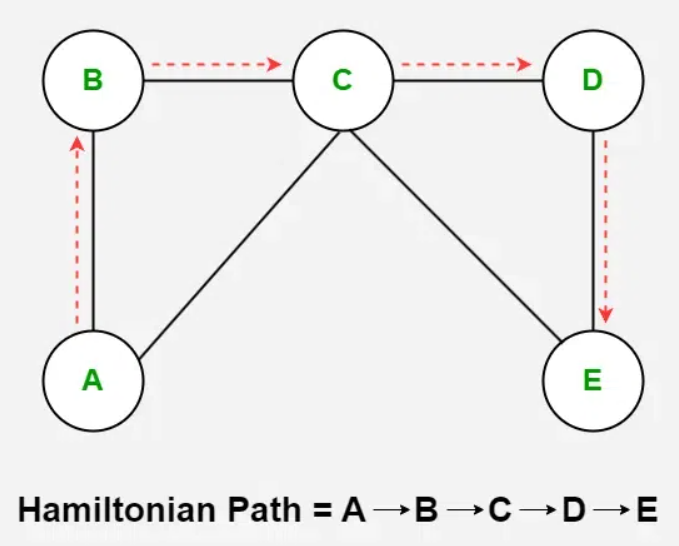
\includegraphics[width=0.3\linewidth]{hampath-example.png}
\end{center}
\begin{theorem}{$HAMPATH$ Problem}
	s\footnotesize
	\begin{center}
		$HAMPATH = \{\langle G,s,t \rangle \mid G \text{ grafo orientato con cammino hamiltoniano da } s \text{ a } t\}$ \\
		$HAMPATH \in \mathcal{NP}$
	\end{center}
	\begin{center}
		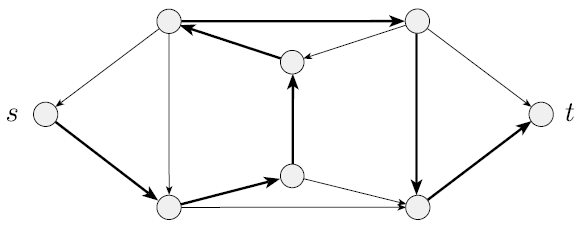
\includegraphics[width=0.7\linewidth]{hampath-problem.png}
	\end{center}
	\begin{ragionamento}
		per dimostrarlo, costruisco una MdT non deterministica che decide $HAMPATH$ in tempo polinomiale (senza certificato).
	\end{ragionamento}
	\begin{proof}
		Sia $H$ una MdT non deterministica che decide $HAMPATH$ in tempo polinomiale come segue. $\langle G,s,t \rangle$ è la codifica binaria
		del grafo orientato $G$ e dei nodi $s,t$ dove $s \neq t$ (codifica come lista di adiacenza o matrice di adiacenza). \\ \\
		$H$ ha 3 nastri:
		\begin{itemize}
			\item \textbf{Nastro 1:} codifica del grafo in input
			\item \textbf{Nastro 2:} contiene sequenza di nodi generate $p_1, \cdots, p_n$ dove $n$ rappresenza il numero di nodi di $G$
			\item \textbf{Nastro 3:} nastro di lavoro; usato per controllare se la sequenza è hamiltoniana (che non ci siano nodi ripetuti)
		\end{itemize}
		$H$ su input $\langle G,s,t \rangle$:
		\begin{enumerate}
			\item $H$ genera una sequenza di nodi e la scrive sul nastro 2.
			\item $H$ usa il nastro 3 per controllare se la sequenza (del nastro 2) è hamiltoniana; se non lo è, rifiuta.
			\item $H$ usa il nastro 2 per controllare se $p_1=s \land p_n=t$; se il controllo fallisce, rifiuta.
			\item $H$ usa il nastro 2 per controllare, se, per la sequenza fornita, gli archi esistono davvero in $G$;
			      Per ogni coppia di nodi consecutiva $(p_i, p_{i+1})$ della sequenza, verifica che esista l'arco corrispondente in $G$; se
			      per qualche $i$ tale arco non esiste, rifiuta. Altrimenti $H$ accetta l'input $\langle G,s,t \rangle$.
		\end{enumerate}
		Analizzo la complessità:
		\begin{enumerate}
			\item Per il passo 1, scrivere un numero binario $n$ costa $O(\log_2n)$. Quindi scrivere una sequenza di $n$ nodi costa $O(n \cdot \log_2n)$
			\item Per il passo 2, viene copiata la sequenza dal nastro 2 al nastro 3 che costa $O(n \cdot \log_2n)$, poi controlla che nessun nodo
			      sia ripetuto, ovvero controllare che tutti i nodi siano distinti $O(n^2\log_2n)$, strategia spiegata nelle note\footnote{
				      Ripeto il ciclo per gli $n$ nodi della sequenza:
				      \begin{enumerate}
					      \item Copiare la codifica del $i$-esimo nodo dal nastro 2 al nastro 3, costo $O(\log_2n)$
					      \item Riportare la testina del nastro 2 all'inizio della sequenza, costo $O(n\log_2n)$
					      \item Scorrere la sequenza degli $n$ nodi confrontandoli con il nodo scritto sul nastro 3, costo $n\cdot O(\log_2n)$ ovvero $O(n \log_2n)$
				      \end{enumerate}
				      Dato che i passi a,b,c sono in sequenza allora ho che la complessità è $O(\log_2n)+O(\log_2n)+O(n\log_2n)$ ovvero $O(n\log_2n)$. Ma il ciclo
				      si deve ripetere per gli $n$ nodi della sequenza, quindi la complessità finale sarà $n\cdot O(n\log_2n)=\textcolor{red}{O(n^2\log_2n)}$. \\
			      }.
			\item Per il passo 3, controlla se $p_1=s \land p_n=t$, costa O($n\log_2n$); strategia spiegata nelle note\footnote{
				      Prima di tutto, so che la testina del nastro 2 è alla fine, e quindi:
				      \begin{enumerate}
					      \item Copio il valore di $s$ dal nastro 1 al nastro 3. La testina del nastro 1 deve fare al massimo $O(n\log_2n)$ spostamenti
					            per arrivare al valore di $s$, poi copiarlo sul nastro 3 costa $O(\log_2n)$. Quindi $O(n\log_2n)+O(\log_2n)=O(n\log_2n)$
					      \item Copio il valore di $t$ dal nastro 1 al nastro 3, stesso costo $O(n\log_2n)$
					      \item Confronto $p_n$ del nastro 2 con $t$ sul nastro 3 muovendo entrambe le testine verso sinistra, costo $O(\log_2n)$
					      \item Muovo la testina del nastro 2 fino all'inizio della sequenza $O(n\log_2n)$
					      \item Confronto $p_1$ del nastro 2 con $s$ sul nastro 3, costo $O(\log_2n)$
				      \end{enumerate}
				      Dato che i passi sono sequenziali, il costo complessivo è: $O(n\log_2n)+O(n\log_2n)+O(\log_2n)+O(n\log_2n)+O(\log_2n)=\textcolor{red}{O(n\log_2n)}$\\
			      }.
			\item Per il passo 4, controlla se gli archi esistono, costa $O(n^2\log_2n)$; strategia spiegata nelle note\footnote{
				      Ripeto il ciclo per ogni coppia $(p_i, p_{i+1})$ quindi per $i=1, \cdots, n-1$:
				      \begin{enumerate}
					      \item Posiziona la testina del nastro 2 sull'$i$-esimo nodo, ovvero su $p_i$, costo $O(n\log_2n)$
					      \item Posiziona la testina del nastro 1 sull'$i$-esimo nodo, costo $O(n\log_2n)$
					      \item Confronta l'$i$-esimo nodo nei due nastri per vedere se si tratta dello stesso, costo $O(\log_2n)$
					      \item Muovi la testina dal nodo $p_i$ al nodo $p_{i+1}$ sul 2 nastro, costo $O(\log_2n)$
					      \item Confronta i nodi della lista di adiacenza dell'$i$-esimo nodo sul nastro 1 con il nodo $p_{i+1}$ del nastro 2; spostamento
					            e lettura per $n$ nodi $O(n\log_2n)$ quindi sul nastro 1 costo $O(n\log_2n)$ con confronto del nastro 2, $O(\log_2n)$; quindi
					            $O(n\log_2n)+O(\log_2n)=O(n\log_2n)$.
				      \end{enumerate}
				      Dato che i passi a-b-c-d-e sono in sequenza allora la complessità è $O(n\log_2n)+O(n\log_2n)+O(\log_2n)+O(\log_2n)+O(n\log_2n)=O(n\log_2n)$. Poi
				      dato che il ciclo va ripetuto per $n-1$ volte allora la complessità finale sarà $(n-1)\cdot(O(n\log_2n))=O(n)\cdot(O(n\log_2n))
					      =\textcolor{red}{O(n^2\log_2n)}$
			      }.
		\end{enumerate}
		\underline{Conclusione:} La complessità finale della MdT $H$ è $tC_H(n)=O(n\log_2n)+O(n^2\log_2n)+O(n\log_2n)+O(n^2\log_2n)=\textcolor{red}{O(n^2\log_2n)}$ dove
		$n$ rappresenta la lunghezza dell'input. Quindi una complessità polinomiale. Ho costruito una MdT $H$ non deterministica che decide $HAMPATH$ in
		tempo polinomiale, pertanto $HAMPATH \in \mathcal{NP}$.
	\end{proof}
	\textcolor{red}{Importante:} $H$ è una MdT non deterministica e quindi questo vuol dire che $H$ esegue i passi dal 1 al 4
	su sequenze diverse in modo parallelo (rami). Ogni sequenza corrisponde a un ramo di computazione, e
	l'input è accettato se almeno un ramo accetta (termina in uno stato accettante).
	$\rule{\linewidth}{0.3pt}$  % linea orizzontale lunga quanto la pagina, spessore 0.4pt$
	Spiegazione dettagliata della MdT non deterministica $H$. \\ \\
	$H$ su input $\langle G,s,t \rangle$:
	\begin{enumerate}
		\item $H$ genera una sequenza di nodi e la scrive sul nastro 2
		\item $H$ usa il nastro 3 per controllare se la sequenza (del nastro 2) è hamiltoniana:
		      \begin{itemize}
			      \item Se sì, vai al passo 3.
			      \item Se no, allora rifiuta la sequenza (questo ramo)
		      \end{itemize}
		\item $H$ usa il nastro 2 per controllare che $p_1=s$ e che $p_n=t$
		      \begin{itemize}
			      \item Se sì, vai al passo 4.
			      \item Se no, allora rifiuta la sequenza (questo ramo)
		      \end{itemize}
		\item $H$ usa il nastro 2 per controllare se per la sequenza fornita, gli archi esistono davvero in $G$;
		      Per ogni coppia di nodi consecutiva $(p_i, p_{i+1})$ nella sequenza, verifica che esista l'arco corrispondente in $G$:
		      \begin{itemize}
			      \item Se sì, allora accetta l'input $\langle G,s,t \rangle$
			      \item Se no, allora rifiuta (questo ramo)
		      \end{itemize}
	\end{enumerate}
\end{theorem}
\begin{theorem}{$HAMPATH$ Problem}
	s\footnotesize
	\begin{center}
		$HAMPATH = \{\langle G,s,t \rangle \mid G \text{ grafo orientato con cammino hamiltoniano da } s \text{ a } t\}$ \\
		$HAMPATH$ è $\mathcal{NP}$-Completo
	\end{center}
	\begin{proof}
		\textcolor{red}{\textbf{1. Dimostrare che $HAMPATH \in \mathcal{NP}$}} \\
		Lo abbiamo già dimostrato sopra. \\ \\
		\textcolor{red}{\textbf{2. Dimostrare che $HAMPATH$ è $\mathcal{NP}$-Hard}} \\
	\end{proof}
\end{theorem}
%%%%%%%%%%%%%%%%%%%%%%%%%%%%%%%%%%%%%%%%%%%%%%%%%%%%%%%%%%%%%%%%%%%%%%%%%%%%%%%%%%%%%%%%%%%%%%%%%%%%%%
%%%%%%%%%%%%%%%%%%%%%%%%%%%%%%%%%%%%%%%%%%%%%%%%%%%%%%%%%%%%%%%%%%%%%%%%%%%%%%%%%%%%%%%%%%%%%%%%%%%%%%
\subsubsection{$HAMCYCLE$}
vedi pg. 476 di SudKamp
%%%%%%%%%%%%%%%%%%%%%%%%%%%%%%%%%%%%%%%%%%%%%%%%%%%%%%%%%%%%%%%%%%%%%%%%%%%%%%%%%%%%%%%%%%%%%%%%%%%%%%
%%%%%%%%%%%%%%%%%%%%%%%%%%%%%%%%%%%%%%%%%%%%%%%%%%%%%%%%%%%%%%%%%%%%%%%%%%%%%%%%%%%%%%%%%%%%%%%%%%%%%%
\subsubsection{$CLIQUE$}
\begin{definition}[Grafo completo]
	Un grafo completo è un grafo non orientato nel quale ogni nodo è collegato a tutti i vertici rimanenti.
	\begin{center}
		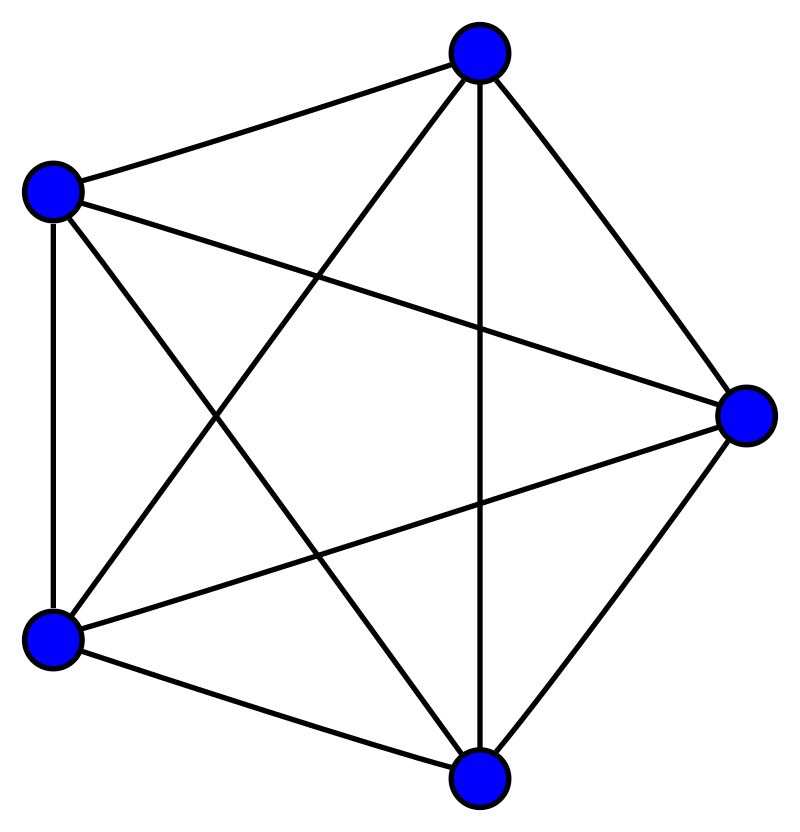
\includegraphics[width=0.2\linewidth]{complete-graph.png}
	\end{center}
\end{definition}
Un \textcolor{red}{clique} è un sottografo completo di un grafo non orientato.
\begin{center}
	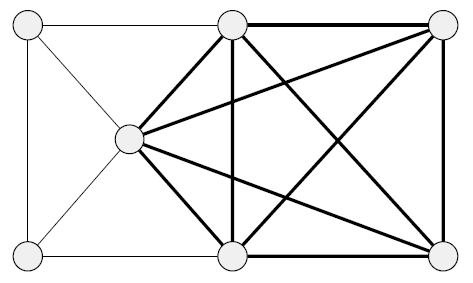
\includegraphics[width=0.3\linewidth]{clique.png}
\end{center}
Un \textcolor{red}{$k$-clique} è un clique che contiene $k$ nodi. (La figura sopra è un 5-clique)
\begin{theorem}{$CLIQUE$ Problem}
	dDato $G$ grafo non orientato, esiste un sottografo completo di $G$ con $k$ vertici?
	\begin{center}
		$CLIQUE = \{\langle G,k \rangle \mid G \text{ grafo non orientato con } k\text{-clique}\}$ \\
		$CLIQUE$ è $\mathcal{NP}$-Completo
	\end{center}
	\footnotesize
	\begin{proof}
		\textcolor{red}{\textbf{1. Dimostrare che $CLIQUE \in \mathcal{NP}$}} \\
		Costruisco una MdT $N$ non deterministica che decide $CLIQUE$ in tempo polinomiale come segue. Sia $G=(V,E)$ un grafo non orientato.
		L'input di \( N \) è la codifica \( \langle G, k \rangle \), dove \( G = (V, E) \) è un grafo non orientato e \( k \in \mathbb{N} \). \\ \\
		$N$ su input $\langle G,k \rangle$:
		\begin{enumerate}
			\item $N$ indovina\footnote{
				      “indovinare” una soluzione, cioè provare tutte le possibilità in parallelo, in senso teorico;
				      Esistono tantissimi sottoinsiemi di $k$ vertici, e dato che la MdT è non deterministica, è possibile
				      provarli tutti in parallelo.
			      } (non deterministicamente) un sottoinsieme $C$ dei vertici di $G$ tale che $|C|=k$
			\item $N$ verifica se i $k$ vertici scelti formano una clique:
			      \begin{itemize}
				      \item Se sì, $N$ termina in uno stato accettante \\
				            $\langle G,k \rangle \in CLIQUE$
				      \item Se no, $N$ termina in uno stato di rifiuto \\
				            $\langle G,k \rangle \notin CLIQUE$
			      \end{itemize}
		\end{enumerate}
		La complessità di $N$ è polinomiale, pertanto $CLIQUE \in \mathcal{NP}$. \\ \\
		\textcolor{red}{\textbf{2. Dimostrare che $CLIQUE$ è $\mathcal{NP}$-Hard}} \\
		Per dimostrare che $CLIQUE$ è $\mathcal{NP}$-Hard, effettuo una riduzione polinomiale da $3-SAT$ (che è $\mathcal{NP}$-Hard)
		a $CLIQUE$, costruendo per ogni formula $\phi$ 3-CNF arbitraria un grafo non orientato; faccio vedere
		che la riduzione funziona perchè $\phi$ è soddisfacibile $\iff$ G ha un $k-clique$. \\
		Effettuo una riduzione da $3-SAT$ a $CLIQUE$:
		\begin{center}
			$3-SAT \leq_p CLIQUE$
		\end{center}
		\begin{itemize}
			\item Sia $\phi$ la 3-CNF formula con $k$ clausole (3 letterali per clausola):
			      \begin{center}
				      $\phi = (a_1 \lor b_1 \lor c_1) \land (a_2 \lor b_2 \lor c_2) \land \cdots \land (a_k \lor b_k \lor c_k)$
			      \end{center}
		\end{itemize}
		\textcolor{red}{2.1 Costruisco la funzione di riduzione $f$} \\
		$f$ riceve come input $\phi$ e genera come output $\langle G,k \rangle$, dove $G$ è un grafo non orientato definito come segue:
		\begin{enumerate}
			\item \textcolor{blue}{\textbf{Costruzione dei nodi di $G$}}
			      \begin{itemize}
				      \item I nodi di $G$ sono organizzati in $k$ gruppi ($k$ è il numero di clausole nella formula) di 3 nodi ciascuno
				      \item Ogni gruppo $t_i$ corrisponde quindi ad una clausola della formila, $t_i=(a_i \lor b_i \lor c_i)$
				      \item Ogni nodo corrisponde ad un letterale della formula $\phi$, quindi in totale $G$ ha $3k$ nodi
			      \end{itemize}
			\item \textcolor{blue}{\textbf{Costruzione degli archi di $G$}} \\
			      Mettiamo archi tra tutte le coppie di nodi, tranne per:
			      \begin{itemize}
				      \item Nodi dello stesso gruppo (niente archi tra letterali della stessa clausola)
				      \item Nodi che rappresentano letterali opposti (niente arco tra $a_i$ e $\overline{a_i}$)
			      \end{itemize}
		\end{enumerate}
		Esempio illustrativo: \\
		Sia $\phi = (x_1 \lor x_1 \lor x_2) \land (\overline{x_1} \lor \overline{x_2} \lor \overline{x_2}) \land (\overline{x_1} \lor x_2 \lor x_2)$. La funzione di riduzione $f$, con input $\phi$,
		produce il seguente grafo:
		\begin{center}
			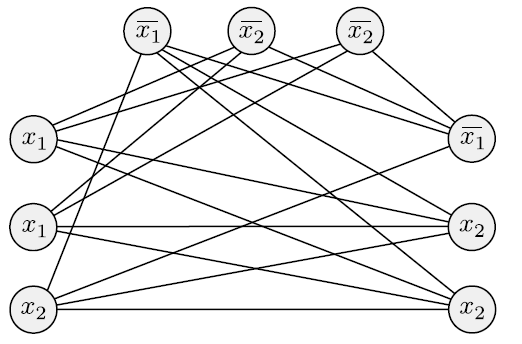
\includegraphics[width=0.5\linewidth]{clique-npcomplete.png} \\
			$\phi$ è soddisfacibile $\iff$ G ha un $k-clique$
		\end{center}

		\textcolor{red}{2.2 Analizzo complessità della funzione di riduzione $f$} \\
		Voglio assicurarmi che $f$ sia una riduzione polinomiale. Ricordiamo che: nota\footnote{\textit{quando analizziamo algoritmi su grafi, possiamo esprimere il tempo di esecuzione
				in base al numero di nodi del grafo, invece che della dimensione della rappresentazione del grafo (cioè della lunghezza dell'input codificato). Esempio: in un problema su grafi,
				l'algoritmo impiega tempo O($v^2$) dove $v$ è il numero di nodi del grafo.}}. \\
		Nel caso peggiore ho complessità $O(n^2)$ dove $n$ è la lunghezza dell'input, e quindi polinomiale. \\ \\
		\textcolor{red}{2.3 Dimostrazione della correttezza della funzione di riduzione $f$} \\
		Costruire la funzione di riduzione polinomiale non basta, dobbiamo anche dimostrare che valga:
		\begin{center}
			$\phi$ è soddisfacibile $\iff$ G ha un $k-clique$
		\end{center}
		\begin{itemize}
			\item \textcolor{blue}{\textbf{($\Longrightarrow$):}}
			      \begin{proof}
				      $\phi$ è soddisfacibile $\implies$ $G$ ha un $k-clique$ \\
				      Per ipotesi, $\phi$ è soddisfacibile e quindi esiste un'assegnazione di valori
				      alle variabili che rende vera ogni clausola.
				      In ogni clausola di $\phi$, almeno un letterale risulta vero. \\
				      In ogni gruppo $t_i$ di $G$ seleziono il nodo corrispondente a un letterale vero (che rende vera la clausola). Se ci sono più letterali veri nella stessa clausola,
				      scelgo arbitrariamente uno tra questi. \\ \textcolor{red}{I nodi appena selezionati formano una $k-clique$:} il numero di nodi selezionati è $k$ perchè ne abbiamo scelto
				      uno per ciascuno dei $k$ gruppi. Inoltre, ogni coppia di nodi selezionati è collegata da un arco, perché nessuna coppia rientra nelle eccezioni descritte in precedenza
				      (stesso gruppo o letterali opposti). \\
				      Pertanto, $G$ ha un $k-clique$.
			      \end{proof}
			\item \textcolor{blue}{\textbf{($\Longleftarrow$):}}
			      \begin{proof}
				      $\phi$ è soddisfacibile $\Longleftarrow$ G ha un $k-clique$ \\
				      Per ipotesi, $G$ ha una $k-clique$ e nessuno dei $k$ nodi della clique è nello stesso gruppo, perchè ricordiamoci che i nodi dello stesso gruppo $t_i$ non
				      sono collegati tra loro. Quindi, ognuno dei $k$ gruppi contiene esattamente un nodo della clique. \\
				      Adesso, assegno il valore 1 ($TRUE$) ai letterali corrispondenti ai nodi della clique.
				      Questo è sempre possibile senza creare contraddizioni, perchè due letterali opposti ($x_i$ e $\overline{x_i}$) non possono entrambi far parte della clique.
				      Quindi la clique non può contenere contraddizioni, e quindi possiamo assegnare i valori di verità in modo coerente.
				      \textcolor{red}{Questa assegnazione soddisfa $\phi$}, perchè ogni gruppo $t_i$ di $G$ contiene un nodo della clique, e quindi ogni clausola contiene
				      almeno un letterale vero (che rende vera la clausola e quindi l'intera formula). \\
				      Pertanto, $\phi$ è soddisfacibile.
			      \end{proof}
		\end{itemize}
		Abbiamo quindi dimostrato che in questa riduzione polinomiale, vale:
		$\phi$ è soddisfacibile $\iff$ G ha un $k-clique$. \\ \\

		\underline{Conclusione:} Ho costruito correttamente una riduzione polinomiale da $3-SAT$ a $CLIQUE$, pertanto $CLIQUE$ è $\mathcal{NP}$-Hard.
		Essendo $CLIQUE \in \mathcal{NP}$ e $\mathcal{NP}$-Hard, segue che $CLIQUE$ è $\mathcal{NP}$-Completo.
	\end{proof}
\end{theorem}
%%%%%%%%%%%%%%%%%%%%%%%%%%%%%%%%%%%%%%%%%%%%%%%%%%%%%%%%%%%%%%%%%%%%%%%%%%%%%%%%%%%%%%%%%%%%%%%%%%%%%%
%%%%%%%%%%%%%%%%%%%%%%%%%%%%%%%%%%%%%%%%%%%%%%%%%%%%%%%%%%%%%%%%%%%%%%%%%%%%%%%%%%%%%%%%%%%%%%%%%%%%%%
\subsubsection{$VERTEX$ $COVER$}
Sia $G=(V,E)$ un grafo non orientato. Scelto un sottoinsieme di vertici $C$ di $V$, si dice "vertex cover" se i nodi di $C$ "coprono/toccano" tutti gli archi del grafo.
\begin{figure}[h]
	\centering
	\begin{subfigure}[b]{0.24\textwidth}
		\centering
		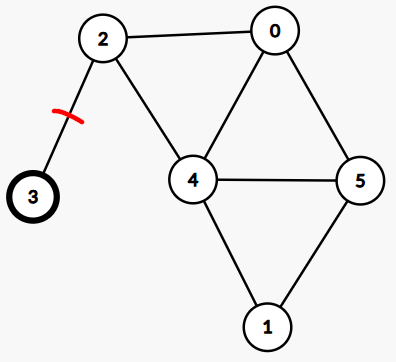
\includegraphics[width=\textwidth]{vc1.png}
		\caption{Passo 1}
	\end{subfigure}
	\hfill
	\begin{subfigure}[b]{0.24\textwidth}
		\centering
		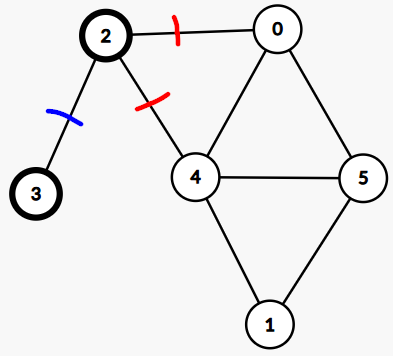
\includegraphics[width=\textwidth]{vc2.png}
		\caption{Passo 2}
	\end{subfigure}
	\hfill
	\begin{subfigure}[b]{0.24\textwidth}
		\centering
		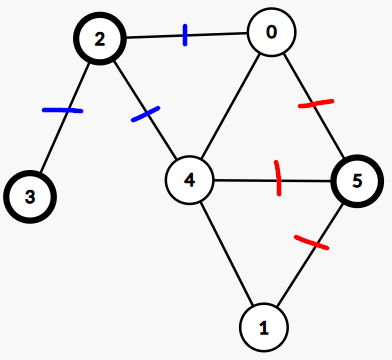
\includegraphics[width=\textwidth]{vc3.png}
		\caption{Passo 3}
	\end{subfigure}
	\hfill
	\begin{subfigure}[b]{0.24\textwidth}
		\centering
		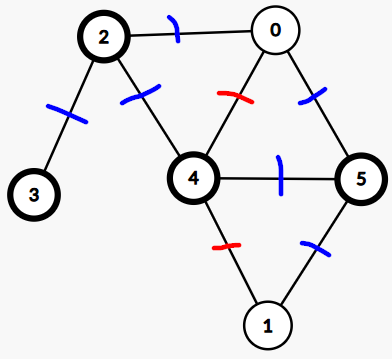
\includegraphics[width=\textwidth]{vc4.png}
		\caption{Passo 4}
	\end{subfigure}
	\caption{L'insieme $C=\{2,3,4,5\}$ è vertex cover}
\end{figure}
\begin{theorem}{$VERTEX$ $COVER$ Problem}
	dDato $G$ grafo non orientato e $k \in \mathbb{N}$, esiste un vertex cover $C$ di $G$ con $k$ vertici?
	\begin{center}
		$VC = \{\langle G,k \rangle \mid G \text{ grafo non orientato con un vertex cover di } k \text{ nodi}\}$ \\
		$VC$ è $\mathcal{NP}$-Completo
	\end{center}
	\footnotesize
	\begin{proof}
		\textcolor{red}{\textbf{1. Dimostrare che $VC \in \mathcal{NP}$}} \\
		Costruisco una MdT $N$ non deterministica che decide $VC$ in tempo polinomiale come segue. Sia $G=(V,E)$ un grafo non orientato.
		L'input di \( N \) è la codifica \( \langle G, k \rangle \), dove \( G = (V, E) \) è un grafo non orientato e \( k \in \mathbb{N} \). \\ \\
		$N$ su input $\langle G, k \rangle$:
		\begin{enumerate}
			\item Non deterministicamente sceglie un insieme $C \subseteq V$ di $k$ vertici.
			\item Per ogni arco $\{x,y\} \in E$, verifica che almeno uno tra $x$ e $y$ appartenga a $C$. \\
			      (Per ogni singolo arco, devo verificare se uno dei due vertici $x,y$ sono in $C$)
			\item Se tutti gli archi sono coperti da $C$, accetta l'input; altrimenti rifiuta.
		\end{enumerate}
		La scelta non deterministica del sottoinsieme $C$ permette di “provare tutte le possibili soluzioni” contemporaneamente.
		La verifica che tutti gli archi siano coperti richiede al massimo $|E| \cdot k$ operazioni ($|E|$ numero totale archi del grafo), quindi è tempo polinomiale rispetto alla dimensione dell'input.
		Ho costruito una MdT non deterministica che decide $VC$ in tempo polinomiale, pertanto $VC \in \mathcal{NP}$. \\ \\
		\textcolor{red}{\textbf{2. Dimostrare che $VC$ è $\mathcal{NP}$-Hard}} \\
		Effetto una riduzione polinomiale da $3-SAT$(che è $\mathcal{NP}$-Hard) a $VC$, costruendo per ogni formula $\phi$ 3-CNF arbitraria un grafo non orientato; faccio
		vedere che la riduzione funziona perchè $\phi$ è soddisfacibile $\iff G$ ha un vertex cover di $k$ nodi.
		\begin{center}
			$3-SAT \leq_p VC$
		\end{center}
		\begin{itemize}
			\item Sia $\phi$ la 3-CNF formula con $l$ clausole (3 letterali per clausola):
			      \begin{center}
				      $\phi = (a_1 \lor b_1 \lor c_1) \land (a_2 \lor b_2 \lor c_2) \land \cdots \land (a_l \lor b_l \lor c_l)$
			      \end{center}
		\end{itemize}
		\textcolor{red}{2.1 Costruisco la funzione di riduzione $f$} \\
		$f$ riceve come input $\phi$ e genera come output $\langle G,k \rangle$, dove $G$ è un grafo non orientato definito come segue:
		\begin{enumerate}
			\item \textcolor{blue}{\textbf{Costruzione dei nodi di $G$}}
			      \begin{enumerate}
				      \item Scrivo un nodo per ogni letterale di ogni clausola (3$l$ nodi)
				      \item Aggiungo altre $m$ coppie di nodi ($m$ numero delle variabili nella formula) che rappresentano le variabili positive e negate (2$m$ nodi)
			      \end{enumerate}
			      Il grafo avrà un totale di $3l+2m$ nodi.
			\item \textcolor{blue}{\textbf{Costruzione degli archi di $G$}} \\
			      Mettiamo archi tra:
			      \begin{enumerate}
				      \item Nodi che rappresentano letterali della stessa clausola (formando i triangoli)
				      \item Nodi che rappresentano letterali opposti (tra $a_i$ e $\overline{a_i}$, le coppie di $m$ nodi)
				      \item Nodi che rappresentano lo stesso letterale tra i triangoli e le coppie di $m$ nodi
			      \end{enumerate}
		\end{enumerate}
		Un vertex cover di $G$ possiede almeno $m+2l$ vertici, perchè:
		\begin{itemize}
			\item Per ogni triangolo di clausola devo scegliere almeno 2 nodi nel vertex cover per coprire tutti gli archi del triangolo
			\item Per ogni coppia di nodi variabile/negazione devo scegliere 1 nodo per coprire l'arco che li collega
		\end{itemize}
		Esempio illustrativo: \\
		Sia $\phi = (x_1 \lor x_1 \lor x_2) \land (\overline{x_1} \lor \overline{x_2} \lor \overline{x_2}) \land (\overline{x_1} \lor x_2 \lor x_2)$. La funzione di riduzione $f$, con input $\phi$,
		produce il seguente grafo:
		\begin{center}
			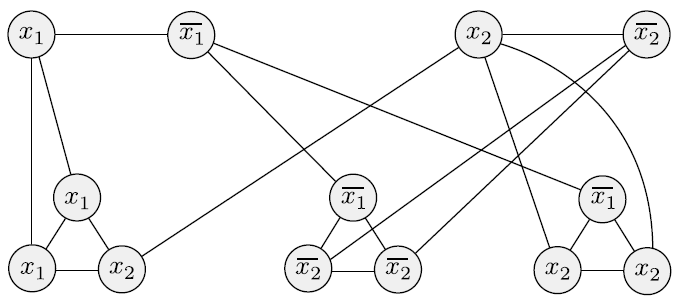
\includegraphics[width=0.7\linewidth]{vertex-cover-ex.png} \\
			$\phi$ è soddisfacibile $\iff$ G ha un vertex cover di $k$ nodi
		\end{center}
		\textcolor{red}{2.2. Analizzo complessità della funzione di riduzione $f$} \\
		Per costruire il grafo si richiede tempo $O(m+l)$, quindi la riduzione è polinomiale.
		\textcolor{red}{2.3. Dimostrazione della correttezza della funzione di riduzione $f$} \\
		Costruire la funzione di riduzione polinomiale non basta, dobbiamo anche dimostrare che valga:
		\begin{center}
			$\phi$ è soddisfacibile $\iff$ G ha un vertex cover di $k$ nodi
		\end{center}
		\begin{itemize}
			\item \textcolor{blue}{\textbf{($\Longrightarrow$):}}
			      \begin{proof}
				      $\phi$ è soddisfacibile $\implies$ $G$ ha un vertex cover di $k$ nodi \\
				      Per ipotesi, $\phi$ è soddisfacibile e quindi esiste un'assegnazione di valori
				      alle variabili che rende vera ogni clausola.
				      In ogni clausola di $\phi$, almeno un letterale risulta vero. \\
				      Adesso faccio vedere che, essendo $\phi$ soddifacibile, posso costruire il vertex cover di $G$ come segue:
				      \begin{enumerate}
					      \item Per prima cosa, per ogni coppia di nodi variabile/negazione scelgo 1 nodo della coppia:
					            \begin{itemize}
						            \item Se nella nostra assegnazione $x_1=true$, allora metto nel vertex cover il nodo che rappresenta $x_i$
						            \item Se invece nella nostra assegnazione $x_i=false$, allora metto nel vc il nodo $\overline{x_i}$
					            \end{itemize}
					            Quindi, alla fine scelgo $m$ nodi ($m$ è il numero di variabili di $\phi$);
					      \item Per ogni clausola (i triangoli), scelgo uno dei letterali che è vero (almeno uno deve esserlo, visto che
					            la formula è soddisfacibile) e metto nel vc gli altri due nodi. \\
					            Quindi, alla fine scelgo $2l$ nodi ($l$ è il numero di clausole di $\phi$)
				      \end{enumerate}
				      Esempio illustrativo: \\
				      Sia $t$ l'assegnamento che rende $\phi$ soddisfacibile: \\
				      $x_1= false, x_2= true$
				      \begin{center}
					      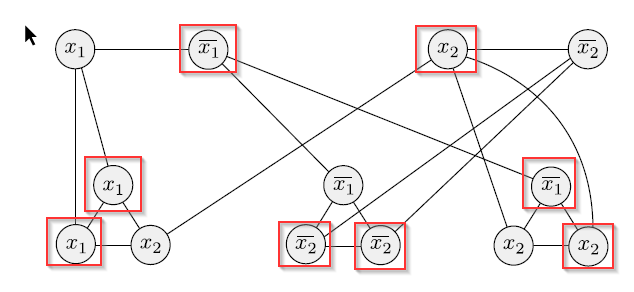
\includegraphics[width=0.8\linewidth]{vc-example.png}
				      \end{center}
				      Quindi, l'insieme di vertici così definito è un vertex cover.  \\
				      Pertanto, $G$ ha un vertex cover di $k=m+2l$ nodi.
			      \end{proof}
			\item \textcolor{blue}{\textbf{($\Longleftarrow$):}}
			      \begin{proof}
				      $\phi$ è soddisfacibile $\Longleftarrow G$ ha un vertex cover di $k$ nodi \\
				      Per ipotesi, $G$ ha un vertex cover di $k$ nodi, mostro che $\phi$ è soddisfacibile costruendo
				      un'assegnazione di valori che la renda vera: \\
				      Osservo i nodi che appartengono al vertex cover e assegno $true$ ai letterali corrispondenti (
				      se nel vc c'è $x_i$, allora assegno $x_i=true$; se invece nel vc c'è $\overline{x_i}$, allora assegno
				      $\overline{x_i}=false$). \\
				      Con questo assegnamento, ogni clausola è soddisfatta dal letterale corrispondente al nodo che non è nel vertex cover
				      di ogni triangolo. \\
				      Pertanto, $\phi$ è soddisfacibile.
			      \end{proof}
		\end{itemize}
		Abbiamo quindi dimostrato che in questa riduzione polinomiale, vale:
		$\phi$ è soddisfacibile $\iff$ $G$ ha un vertex cover di $k$ nodi. \\ \\

		\underline{Conclusione:} Ho costruito correttamente una riduzione polinomiale da $3-SAT$ a $VC$, pertanto $VC$ è $\mathcal{NP}$-Hard.
		Essendo $VC \in \mathcal{NP}$ e $\mathcal{NP}$-Hard, segue che $VC$ è $\mathcal{NP}$-Completo.
	\end{proof}
\end{theorem}
%%%%%%%%%%%%%%%%%%%%%%%%%%%%%%%%%%%%%%%%%%%%%%%%%%%%%%%%%%%%%%%%%%%%%%%%%%%%%%%%%%%%%%%%%%%%%%%%%%%%%%
%%%%%%%%%%%%%%%%%%%%%%%%%%%%%%%%%%%%%%%%%%%%%%%%%%%%%%%%%%%%%%%%%%%%%%%%%%%%%%%%%%%%%%%%%%%%%%%%%%%%%%
\break
%%%%%%%%%%%%%%%%%%%%%%%%%%%%%%%%%%%%%%%%%%%%%%%%%%%%%%%%%%%%%%%%%%%%%%%%%%%%%%%%%%%%%%%%%%%%%%%%%%%%%%
%%%%%%%%%%%%%%%%%%%%%%%%%%%%%%%%%%%%%%%%%%%%%%%%%%%%%%%%%%%%%%%%%%%%%%%%%%%%%%%%%%%%%%%%%%%%%%%%%%%%%%
\subsection{Come capire quali problemi sono riducibili ad altri (trucchi)}
%%%%%%%%%%%%%%%%%%%%%%%%%%%%%%%%%%%%%%%%%%%%%%%%%%%%%%%%%%%%%%%%%%%%%%%%%%%%%%%%%%%%%%%%%%%%%%%%%%%%%%
%%%%%%%%%%%%%%%%%%%%%%%%%%%%%%%%%%%%%%%%%%%%%%%%%%%%%%%%%%%%%%%%%%%%%%%%%%%%%%%%%%%%%%%%%%%%%%%%%%%%%%
\subsection{$\mathcal{P}$ vs $\mathcal{NP}$}
La differenza sostanziale tra $\mathcal{P}$ e $\mathcal{NP}$ è:
\begin{itemize}
	\item la classe $\mathcal{P}$ è l'insieme dei problemi \textcolor{red}{\textit{risolvibili}} da una MdT deterministica in tempo polinomiale.
	\item la classe $\mathcal{NP}$ è l'insieme dei problemi \textcolor{red}{\textit{risolvibili}} da una MdT non deterministica in tempo polinomiale (senza
	      certificato); oppure,\textcolor{red}{\textit{ verificabili}} da una MdT deterministica in tempo polinomiale, dato un certificato.
\end{itemize}
Ovvero, se $C \in \mathcal{NP}$:
\begin{itemize}
	\item $\nexists$ un algoritmo deterministico che decide $C$ in tempo polinomiale
	\item $\exists$ un algoritmo deterministico che decide $C$ in tempo esponenziale (o la complessità è piu grande di exp?)
	\item $\exists$ un algoritmo deterministico che verifica un certificato per $C$ in tempo polinomiale
	\item $\exists$ un algoritmo non deterministico che decide $C$ in tempo polinomiale (senza un certificato)
\end{itemize}


\subsection{$\mathcal{P} \neq \mathcal{NP}$}
\subsubsection{$\mathcal{P} \overset{?}{=} \mathcal{NP}$}
%%%%%%%%%%%%%%%%%%%%%%%%%%%%%%%%%%%%%%%%%%%%%%%%%%%%%%%%%%%%%%%%%%%%%%%%%%%%%%%%%%%%%%%%%%%%%%%%%%%%%%
%%%%%%%%%%%%%%%%%%%%%%%%%%%%%%%%%%%%%%%%%%%%%%%%%%%%%%%%%%%%%%%%%%%%%%%%%%%%%%%%%%%%%%%%%%%%%%%%%%%%%%
\break
%%%%%%%%%%%%%%%%%%%%%%%%%%%%%%%%%%%%%%%%%%%%%%%%%%%%%%%%%%%%%%%%%%%%%%%%%%%%%%%%%%%%%%%%%%%%%%%%%%%%%%
%%%%%%%%%%%%%%%%%%%%%%%%%%%%%%%%%%%%%%%%%%%%%%%%%%%%%%%%%%%%%%%%%%%%%%%%%%%%%%%%%%%%%%%%%%%%%%%%%%%%%%
\section{Complessità Spaziale}
\end{document}
